% Judul dokumen
\title{Buku Tugas Akhir ITS}
\author{Utomo, Satrio Heru}

% Pengaturan ukuran teks dan bentuk halaman dua sisi
\documentclass[12pt,twoside]{report}

% Pengaturan ukuran halaman dan margin
\usepackage[a4paper,top=30mm,left=30mm,right=20mm,bottom=25mm]{geometry}

% Pengaturan ukuran spasi
\usepackage[singlespacing]{setspace}

% Pengaturan detail pada file PDF
\usepackage[pdfauthor={\@author},bookmarksnumbered,pdfborder={0 0 0}]{hyperref}

% Pengaturan jenis karakter
\usepackage[utf8]{inputenc}

% Pengaturan pewarnaan
\usepackage[table,xcdraw]{xcolor}

% Pengaturan kutipan artikel
\usepackage[style=apa, backend=biber]{biblatex}

% Package lainnya
\usepackage{changepage}
\usepackage{enumitem}
\usepackage{eso-pic}
\usepackage{txfonts} % Font times
\usepackage{etoolbox}
\usepackage{graphicx}
\usepackage{lipsum}
\usepackage{longtable}
\usepackage{tabularx}
\usepackage{wrapfig}
\usepackage{float}
\usepackage{multicol} % Pembuatan kolom ganda
\usepackage{multirow} % Pembuatan baris ganda
\usepackage[OT1]{fontenc} % Untuk mengatur jenis font dan encodingnya
\usepackage{wrapfig}
\usepackage{float}
\usepackage[section]{placeins}

\usepackage[titles]{tocloft}
\usepackage{subfig}
\setlength{\cftsecindent}{2em}
\setlength{\cftsubsecindent}{2em}
\setlength{\cftbeforechapskip}{1.5ex}
\setlength{\cftbeforesecskip}{1.5ex}
\setlength{\cftbeforetoctitleskip}{0cm}
\setlength{\cftbeforeloftitleskip}{0cm}
\setlength{\cftbeforelottitleskip}{0cm}
\renewcommand{\cfttoctitlefont}{\hfill\Large\bfseries} % command untuk membuat heading bold dan besar
\renewcommand{\cftaftertoctitle}{\hfill}
\renewcommand{\cftloftitlefont}{\hfill\Large\bfseries}
\renewcommand{\cftafterloftitle}{\hfill}
\renewcommand{\cftlottitlefont}{\hfill\Large\bfseries}
\renewcommand{\cftafterlottitle}{\hfill}

% Definisi untuk "Hati ini sengaja dikosongkan"
\patchcmd{\cleardoublepage}{\hbox{}}{
  \thispagestyle{empty}
  \vspace*{\fill}
  \begin{center}\textit{[Halaman ini sengaja dikosongkan]}\end{center}
  \vfill}{}{}

% Pengaturan penomoran halaman
\usepackage{fancyhdr}
\fancyhf{}
\renewcommand{\headrulewidth}{0pt}
\pagestyle{fancy}
\fancyfoot[LE,RO]{\thepage}
\patchcmd{\chapter}{plain}{fancy}{}{}
\patchcmd{\chapter}{empty}{plain}{}{}

% Command untuk bulan
\newcommand{\MONTH}{%
  \ifcase\the\month
  \or Januari% 1
  \or Februari% 2
  \or Maret% 3
  \or April% 4
  \or Mei% 5
  \or Juni% 6
  \or Juli% 7
  \or Agustus% 8
  \or September% 9
  \or Oktober% 10
  \or November% 11
  \or Desember% 12
  \fi}
\newcommand{\ENGMONTH}{%
  \ifcase\the\month
  \or January% 1
  \or February% 2
  \or March% 3
  \or April% 4
  \or May% 5
  \or June% 6
  \or July% 7
  \or August% 8
  \or September% 9
  \or October% 10
  \or November% 11
  \or December% 12
  \fi}

% Pengaturan format judul bab
\usepackage{titlesec}
\titleformat{\chapter}[display]{\bfseries\Large}{BAB \centering\Roman{chapter}}{0ex}{\vspace{0ex}\centering}
\titleformat{\section}{\bfseries\large}{\MakeUppercase{\thesection}}{1ex}{\vspace{1ex}}
\titleformat{\subsection}{\bfseries\large}{\MakeUppercase{\thesubsection}}{1ex}{}
\titleformat{\subsubsection}{\bfseries\large}{\MakeUppercase{\thesubsubsection}}{1ex}{}
\titlespacing{\chapter}{0ex}{0ex}{4ex}
\titlespacing{\section}{0ex}{1ex}{0ex}
\titlespacing{\subsection}{0ex}{0.5ex}{0ex}
\titlespacing{\subsubsection}{0ex}{0.5ex}{0ex}

% Atur variabel berikut sesuai namanya

% nama
\newcommand{\name}{Satrio Heru Utomo}
\newcommand{\authorname}{Utomo, Satrio Heru}
\newcommand{\nickname}{Satrio}
\newcommand{\advisor}{Dr. Supeno Mardi Susiki Nugroho, ST., MT.}
\newcommand{\coadvisor}{Reza Fuad Rachmadi, S.T., M.T., Ph.D}
\newcommand{\examinerone}{Dosen, S.T., M.T.}
\newcommand{\examinertwo}{Dosen, S.T., M.Sc.}
\newcommand{\examinerthree}{Dosen, S.T., M.T.}
\newcommand{\headofdepartment}{Prof. Dosen, S.T., M.T}

% identitas
\newcommand{\nrp}{0721 19 4000 0053}
\newcommand{\advisornip}{19700313 199512 1 001}
\newcommand{\coadvisornip}{19850403 201212 1 001}
\newcommand{\examineronenip}{18560710 194301 1 001}
\newcommand{\examinertwonip}{18560710 194301 1 001}
\newcommand{\examinerthreenip}{18560710 194301 1 001}
\newcommand{\headofdepartmentnip}{18810313 196901 1 001}

% judul
\newcommand{\tatitle}{ANALISIS RETINOPATI DIABETIK DENGAN IMPLEMENTASI MENGGUNAKAN \emph{RESIDUAL NEURAL NETWORK}}
\newcommand{\engtatitle}{\emph{ANALYSIS OF DIABETIC RETINOPATHY WITH IMPLEMENTATION USING RESIDUAL NEURAL NETWORK}}

% tempat
\newcommand{\place}{Surabaya}

% jurusan
\newcommand{\studyprogram}{Teknik Komputer}
\newcommand{\engstudyprogram}{Computer Engineering}

% fakultas
\newcommand{\faculty}{Teknologi Elektro dan Informatika Cerdas}
\newcommand{\engfaculty}{Electrical Engineering and Intelligent Informatics}

% singkatan fakultas
\newcommand{\facultyshort}{FTEIC}
\newcommand{\engfacultyshort}{ELECTICS}

% departemen
\newcommand{\department}{Teknik Komputer}
\newcommand{\engdepartment}{Computer Engineering}

% kode mata kuliah
\newcommand{\coursecode}{EC234701}

% Tambahkan format tanda hubung yang benar di sini
\hyphenation{
  ro-ket
  me-ngem-bang-kan
  per-hi-tu-ngan
  tek-no-lo-gi
  me-la-ku-kan
  ber-so-si-al-i-sa-si
}

% Menambahkan resource daftar pustaka
\addbibresource{pustaka/pustaka.bib}

% Pengaturan format potongan kode
\usepackage{listings}
\definecolor{comment}{RGB}{0,128,0}
\definecolor{string}{RGB}{255,0,0}
\definecolor{keyword}{RGB}{0,0,255}
\lstdefinestyle{codestyle}{
  commentstyle=\color{comment},
  stringstyle=\color{string},
  keywordstyle=\color{keyword},
  basicstyle=\footnotesize\ttfamily,
  numbers=left,
  numberstyle=\tiny,
  numbersep=5pt,
  frame=lines,
  breaklines=true,
  prebreak=\raisebox{0ex}[0ex][0ex]{\ensuremath{\hookleftarrow}},
  showstringspaces=false,
  upquote=true,
  tabsize=2,
}
\lstset{style=codestyle}

% Isi keseluruhan dokumen
\begin{document}

% Sampul luar Bahasa Indonesia
\newcommand\covercontents{sampul/konten-id.tex}
\AddToShipoutPictureBG*{
  \AtPageLowerLeft{
    % Ubah nilai berikut jika posisi horizontal background tidak sesuai
    \hspace{-3.25mm}

    % Ubah nilai berikut jika posisi vertikal background tidak sesuai
    \raisebox{0mm}{
      
\includegraphics[width=\paperwidth,height=\paperheight]{sampul/gambar/sampul-luar-tipis.png}
    }
  }
}

% Menyembunyikan nomor halaman
\thispagestyle{empty}

% Pengaturan margin untuk menyesuaikan konten sampul
\newgeometry{
  top=65mm,
  left=30mm,
  right=30mm,
  bottom=20mm
}

\begin{flushleft}

  % Pemilihan font sans serif
  \sffamily

  % Pemilihan font bold
  \fontseries{bx}
  \selectfont
  \begin{spacing}{1.5}
    \input{\covercontents}
  \end{spacing}

\end{flushleft}

\restoregeometry


% Atur ulang penomoran halaman
\setcounter{page}{1}

% Sampul dalam Bahasa Indonesia
\renewcommand\covercontents{sampul/konten-id.tex}
\AddToShipoutPictureBG*{
  \AtPageLowerLeft{
    % Ubah nilai berikut jika posisi horizontal background tidak sesuai
    \hspace{-4mm}

    % Ubah nilai berikut jika posisi vertikal background tidak sesuai
    \raisebox{0mm}{
      
\includegraphics[width=\paperwidth,height=\paperheight]{sampul/gambar/sampul-luar-tipis.png}
    }
  }
}

% Menyembunyikan nomor halaman
\thispagestyle{empty}

% Pengaturan margin untuk menyesuaikan konten sampul
\newgeometry{
  top=65mm,
  left=30mm,
  right=30mm,
  bottom=20mm
}

\begin{flushleft}

  % Pemilihan font sans serif
  \sffamily

  % Pemilihan font bold
  \fontseries{bx}
  \selectfont
  \begin{spacing}{1.5}
    \input{\covercontents}
  \end{spacing}

\end{flushleft}

\restoregeometry

\clearpage
\cleardoublepage

% Sampul dalam Bahasa Inggris
\renewcommand\covercontents{sampul/konten-en.tex}
\AddToShipoutPictureBG*{
  \AtPageLowerLeft{
    % Ubah nilai berikut jika posisi horizontal background tidak sesuai
    \hspace{-4mm}

    % Ubah nilai berikut jika posisi vertikal background tidak sesuai
    \raisebox{0mm}{
      
\includegraphics[width=\paperwidth,height=\paperheight]{sampul/gambar/sampul-luar-tipis.png}
    }
  }
}

% Menyembunyikan nomor halaman
\thispagestyle{empty}

% Pengaturan margin untuk menyesuaikan konten sampul
\newgeometry{
  top=65mm,
  left=30mm,
  right=30mm,
  bottom=20mm
}

\begin{flushleft}

  % Pemilihan font sans serif
  \sffamily

  % Pemilihan font bold
  \fontseries{bx}
  \selectfont
  \begin{spacing}{1.5}
    \input{\covercontents}
  \end{spacing}

\end{flushleft}

\restoregeometry

\cleardoublepage

% Label tabel dan gambar dalam bahasa indonesia
\renewcommand{\figurename}{Gambar}
\renewcommand{\tablename}{}

% Pengaturan ukuran indentasi paragraf
\setlength{\parindent}{2em}

% Pengaturan ukuran spasi paragraf
\setlength{\parskip}{1ex}

% Lembar pengesahan
\chapter*{LEMBAR PENGESAHAN}

% Menyembunyikan nomor halaman
\thispagestyle{empty}

\begin{center}
  % Ubah kalimat berikut dengan judul tugas akhir
  \textbf{\tatitle{}}
\end{center}

\begingroup
% Pemilihan font ukuran small
\small

\begin{center}
  % Ubah kalimat berikut dengan pernyataan untuk lembar pengesahan
  \textbf{PROPOSAL TUGAS AKHIR} \\
  Diajukan untuk memenuhi salah satu syarat memperoleh gelar
  Sarjana Teknik pada
  Program Studi S-1 \studyprogram{} \\
  Departemen \department{} \\
  Fakultas \faculty{} \\
  Institut Teknologi Sepuluh Nopember
\end{center}

\begin{center}
  % Ubah kalimat berikut dengan nama dan NRP mahasiswa
  Oleh: \textbf{\name{}} \\
  NRP. \nrp{}
\end{center}

\begin{center}
  Disetujui Oleh:
\end{center}

\vspace{10ex}

\begingroup
% Menghilangkan padding
\setlength{\tabcolsep}{0pt}

\noindent
\begin{tabularx}{\textwidth}{X c}
  % Ubah kalimat-kalimat berikut dengan nama dan NIP dosen pembimbing pertama
  \advisor{}           &                 \\
  NIP: \advisornip{}   & (Pembimbing)    \\
                       &                 \\
                       &                 \\
                       &                 \\
  % Ubah kalimat-kalimat berikut dengan nama dan NIP dosen pembimbing kedua
  \coadvisor{}         &                 \\
  NIP: \coadvisornip{} & (Ko-Pembimbing) \\
\end{tabularx}
\endgroup

\vspace{\fill}

\begin{center}
  % Ubah text dibawah menjadi tempat dan tanggal
  \textbf{\MakeUppercase{\place}} \\
  \textbf{\MONTH{}, \the\year{}}
\end{center}
\endgroup

\cleardoublepage
\begin{center}
  \large
  \textbf{APPROVAL SHEET}
\end{center}

% Menyembunyikan nomor halaman
\thispagestyle{empty}

\begin{center}
  \textbf{\engtatitle{}}
\end{center}

\begingroup
% Pemilihan font ukuran small
\small

\begin{center}
  \textbf{FINAL PROJECT}
  \\Submitted to fulfill one of the requirements \\
  for obtaining a degree Bachelor of Engineering at \\
  Undergraduate Study Program of \engstudyprogram{} \\
  Department of \engdepartment{} \\
  Faculty of \engfaculty{} \\
  Sepuluh Nopember Institute of Technology
\end{center}

\begin{center}
  By: \textbf{\name{}}
  \\NRP. \nrp{}
\end{center}

\begin{center}
  Approved by Final Project Examiner Team:
\end{center}

\begingroup
% Menghilangkan padding
\setlength{\tabcolsep}{0pt}

\noindent
\begin{tabularx}{\textwidth}{X l}
  \advisor{}               & (Advisor I)                         \\
  NIP: \advisornip{}       &                                     \\
                           & ................................... \\
                           &                                     \\
                           &                                     \\
  \coadvisor{}             & (Advisor II)                        \\
  NIP: \coadvisornip{}     &                                     \\
                           & ................................... \\
                           &                                     \\
                           &                                     \\
                           & (Examiner I)                        \\
  NIP:                     &                                     \\
                           & ................................... \\
                           &                                     \\
                           &                                     \\
                           & (Examiner II)                       \\
  NIP:                     &                                     \\
                           & ................................... \\
                           &                                     \\
                           & (Examiner II)                       \\
  NIP:                     &                                     \\
                           & ................................... \\
\end{tabularx}
\endgroup

\begin{center}
  Acknowledged, \\
  Head of \engdepartment{} Department \engfacultyshort{} - ITS \\
  
  \vspace{8ex}
  
  \underline{\headofdepartment{}.} \\
  NIP. \headofdepartmentnip{}
\end{center}

\begin{center}
  \textbf{\MakeUppercase{\place{}}\\\ENGMONTH{}, \the\year{}}
\end{center}
\endgroup
\cleardoublepage

% Pernyataan keaslian
\begin{center}
  \large
  \textbf{PERNYATAAN ORISINALITAS}
\end{center}

% Menyembunyikan nomor halaman
\thispagestyle{empty}

\vspace{2ex}

% Ubah paragraf-paragraf berikut sesuai dengan yang ingin diisi pada pernyataan keaslian

\noindent Yang bertanda tangan dibawah ini:

\noindent\begin{tabularx}{\textwidth}{l l X}
                         &   &                            \\
  Nama Mahasiswa / NRP   & : & \name{} / \nrp{}           \\
  Departemen             & : & \department{}              \\
  Dosen Pembimbing / NIP & : & \advisor{} / \advisornip{} \\
                         &   &                            \\
\end{tabularx}

Dengan ini menyatakan bahwa Tugas Akhir dengan judul "\tatitle{}" adalah hasil karya sendiri, berfsifat orisinal, dan ditulis dengan mengikuti kaidah penulisan ilmiah.

Bilamana di kemudian hari ditemukan ketidaksesuaian dengan pernyataan ini, maka saya bersedia menerima sanksi sesuai dengan ketentuan yang berlaku di Institut Teknologi Sepuluh Nopember.

\vspace{8ex}

\noindent\begin{tabularx}{\textwidth}{X l}
                     & \place{}, \MONTH{} \the\year{} \\
                     &                                   \\
  Mengetahui         &                                   \\
  Dosen Pembimbing   & Mahasiswa                         \\
                     &                                   \\
                     &                                   \\
                     &                                   \\
                     &                                   \\
                     &                                   \\
  \advisor{}         & \name{}                           \\
  NIP. \advisornip{} & NRP. \nrp{}                       \\
\end{tabularx}

\cleardoublepage
\begin{center}
  \large
  \textbf{STATEMENT OF ORIGINALITY}
\end{center}

% Menyembunyikan nomor halaman
\thispagestyle{empty}

\vspace{2ex}

% Ubah paragraf-paragraf berikut sesuai dengan yang ingin diisi pada pernyataan keaslian

\noindent The undersigned below:

\noindent\begin{tabularx}{\textwidth}{l l X}
                        &   &                            \\
  Name of student / NRP & : & \name{} / \nrp{}           \\
  Department            & : & \engdepartment{}           \\
  Advisor / NIP         & : & \advisor{} / \advisornip{} \\
                        &   &                            \\
\end{tabularx}

Hereby declared that the Final Project with the title of "\engtatitle{}" is the result of my own work, is original, and is written by following the rules of scientific writing.

If in future there is a discrepancy with this statement, then I am willing to accept sanctions in accordance with provisions that apply at Sepuluh Nopember Institute of Technology.

\vspace{8ex}

\noindent\begin{tabularx}{\textwidth}{X l}
                     & \place{},   \ENGMONTH{} \the\year{} \\
                     &                                   \\
  Acknowledged       &                                   \\
  Advisor            & Student                           \\
                     &                                   \\
                     &                                   \\
                     &                                   \\
                     &                                   \\
                     &                                   \\
  \advisor{}         & \name{}                           \\
  NIP. \advisornip{} & NRP. \nrp{}                       \\
\end{tabularx}
\cleardoublepage

% Nomor halaman pembuka dimulai dari sini
\pagenumbering{roman}

% Abstrak Bahasa Indonesia
\begin{center}
  \large\textbf{ABSTRAK}
\end{center}

\addcontentsline{toc}{chapter}{ABSTRAK}

\vspace{2ex}

\begingroup
% Menghilangkan padding
\setlength{\tabcolsep}{0pt}

\noindent
\begin{tabularx}{\textwidth}{l >{\centering}m{2em} X}
  Nama Mahasiswa    & : & \name{}         \\

  Judul Tugas Akhir & : & \tatitle{}      \\

  Pembimbing        & : & 1. \advisor{}   \\
                    &   & 2. \coadvisor{} \\
\end{tabularx}
\endgroup

% Ubah paragraf berikut dengan abstrak dari tugas akhir
\emph{Retinopati diabetik (DR) adalah komplikasi mikrovaskular diabetes dan merupakan penyebab utama kebutaan di antara orang dewasa usia kerja di seluruh dunia. Deteksi dan intervensi dini sangat penting untuk mencegah kehilangan penglihatan dan meningkatkan hasil pengobatan pasien. Namun, metode skrining tradisional sering kali memiliki keterbatasan dalam hal akurasi dan aksesibilitas. Penelitian ini mengusulkan penerapan Residual Neural Network (ResNet) untuk deteksi dan klasifikasi DR secara otomatis dari gambar fundus. Penelitian ini bertujuan untuk berkontribusi pada kemajuan diagnosis DR otomatis dan pada akhirnya meningkatkan perawatan pasien melalui intervensi dini dan strategi perawatan yang dipersonalisasi. Model paling akurat yang dicapai adalah ResNet-18 yang memiliki akurasi validasi terbaik tanpa penyesuaian apa pun pada beban class, dengan nilai 0,8211. Selain itu, model dengan skor Kappa tertinggi adalah model ResNet-18 yang memiliki akurasi Training terbaik tanpa modifikasi apa pun pada beban class, yang menghasilkan nilai Kappa sebesar 0,7584.}

% Ubah kata-kata berikut dengan kata kunci dari tugas akhir
\textbf{Kata Kunci: \emph{Retinopati Diabetik, ResNet, Deep Learning, Analisis Angiografi OCT}}

\cleardoublepage

% Abstrak Bahasa Inggris
\begin{center}
  \large\textbf{ABSTRACT}
\end{center}

\addcontentsline{toc}{chapter}{ABSTRACT}

\vspace{2ex}

\begingroup
% Menghilangkan padding
\setlength{\tabcolsep}{0pt}

\noindent
\begin{tabularx}{\textwidth}{l >{\centering}m{3em} X}
  \emph{Name}     & : & \name{}         \\

  \emph{Title}    & : & \engtatitle{}   \\

  \emph{Advisors} & : & 1. \advisor{}   \\
                  &   & 2. \coadvisor{} \\
\end{tabularx}
\endgroup

% Ubah paragraf berikut dengan abstrak dari tugas akhir dalam Bahasa Inggris
\emph{Diabetic retinopathy (DR) is a microvascular complication of diabetes and is the leading cause of blindness among working-age adults worldwide. Early detection and intervention are crucial to prevent vision loss and improve patient outcomes. However, traditional screening methods often face limitations in accuracy and accessibility. This study proposes the implementation of a Residual Neural Network (ResNet) for automated DR detection and classification from fundus images. By achieving these objectives, this study aims to contribute to the advancement of automated DR diagnosis and ultimately improve patient care through early intervention and personalized treatment strategies.The most accurate model, ResNet-18, achieved the best validation accuracy without any adjustment to the class weight, with a value of 0.8211. Additionally, the model with the highest Kappa score was ResNet-18, which had the best training accuracy without any modification to the class weight, resulting in a Kappa score of 0.7584.}

% Ubah kata-kata berikut dengan kata kunci dari tugas akhir dalam Bahasa Inggris
\textbf{Keywords: \emph{Diabetic retinopathy, ResNet, Deep Learning, Optical Coherence Tomography Angiography Analysis}}
\cleardoublepage

% Kata pengantar
\begin{center}
  \Large
  \textbf{KATA PENGANTAR}
\end{center}

\addcontentsline{toc}{chapter}{KATA PENGANTAR}

\vspace{2ex}

% Ubah paragraf-paragraf berikut dengan isi dari kata pengantar

Puji dan syukur penulis ucapkan kepada Tuhan Yang Maha Esa karena berkat rahmat-Nya dapat diselesaikan penelitian serta penyusunan tugas akhir ini yang berjudul "Analisis Retinopati Diabetik dengan Implementasi Menggunakan \emph{Residual Neural Network}."

Penelitian ini disusun dalam rangka pemenuhan bidang riset di Departemen Teknik Komputer dan persyaratan untuk menyelesaikan pendidikan S1. Dalam pelaksanaan penelitian serta penyusunan buku ini, penulis ingin mengucapkan terima kasih kepada:

\begin{enumerate}[nolistsep]

  \item Keluarga yang telah mendukung penulis hingga mencapai titik ini.

  \item Bapak Supeno Mardi Susiki Nugroho, S.T., M.T. dan Bapak Reza Fuad Rachmadi, S.T., M.T., Ph. D selaku pembimbing yang telah membantu mengarahkan penulis selama pengerjaan dan penyusunan buku ini. 

  \item Bapak Dr. Supeno Mardi Susiki Nugroho, S.T., M.T. selaku Kepala Departemen Teknik Komputer, Fakultas Teknologi Elektro dan Informatika Cerdas, Institut Teknologi Sepuluh Nopember Surabaya, yang telah memberikan kesempatan bagi penulis untuk melakukan serta menyelesaikan tugas akhir ini.
  
  \item Bapak dan Ibu dosen di Departemen Teknik Komputer, yang telah memberikan ilmu bagi penulis sehingga dapat dipahami berbagai macam bidang yang diperlukan untuk melaksanakan dan menyelesaikan tugas akhir ini.

  \item Seluruh sahabat dan teman-teman mahasiswa dan staf di ITS, terutama teman-teman Teknik Komputer yang telah membantu penulis dalam berbagai tahap pada pelaksanaan serta penyusunan tugas akhir ini.

\end{enumerate}

Akhir kata, Penulis harap penelitian ini dapat bermanfaat dan berguna untuk sebanyak mungkin orang. Penulis sadar bahwa buku ini masih belum sempurna oleh karena itu diharapkan dapat diberikan kritik dan saran sehingga penulis dapat lebih meningkatkan kualitas keluaran penulis untuk kedepannya.

\begin{flushright}
  \begin{tabular}[b]{c}
    \place{}, \MONTH{} \the\year{} \\
    \\
    \\
    \\
    \\
    \name{}
  \end{tabular}
\end{flushright}

\cleardoublepage

% Daftar isi
\renewcommand*\contentsname{DAFTAR ISI}
\addcontentsline{toc}{chapter}{\contentsname}
\tableofcontents
\cleardoublepage

% Daftar gambar
\renewcommand*\listfigurename{DAFTAR GAMBAR}
\addcontentsline{toc}{chapter}{\listfigurename}
\listoffigures
\cleardoublepage

% Daftar tabel
\renewcommand*\listtablename{DAFTAR TABEL}
\addcontentsline{toc}{chapter}{\listtablename}
\listoftables
\cleardoublepage

% Nomor halaman isi dimulai dari sini
\pagenumbering{arabic}

% Bab 1 pendahuluan
\chapter{PENDAHULUAN}
\label{chap:pendahuluan}

% Ubah bagian-bagian berikut dengan isi dari pendahuluan

Penelitian ini dilatarbelakangi oleh beberapa kondisi yang menjadi acuan. Terdapat beberapa permasalahan yang terkait dengan acuan tersebut, batasan dari permasalahan tersebut, serta terdapat tujuan dan manfaat yang akan dibahas dan dijawab sebagai hasil dari penelitian ini.

\section{Latar Belakang}
\label{sec:latarbelakang}

Pada era teknologi digital saat ini, penggunaan kecerdasan buatan sangatlah erat pada aspek kehidupan manusia. Mulai dari membantu produktifitas seperti: rekomendasi konten pada social media, asisten virtual, filter spam; meningkatkan efisiensi, seperti: system transportasi cerdas dan penjadwalan otomatis; hiburan, dan dalam sektor penelitian dan pengembangan dalam sains dan teknologi.

Retinopati diabetik adalah komplikasi mikrovaskular diabetes melitus (DM) yang disebabkan oleh kerusakan pembuluh darah di retina. Penyakit ini dapat menyebabkan penurunan penglihatan, bahkan kebutaan \parencite{Yusran2022}. Menurut Organisasi Kesehatan Dunia (WHO), sekitar 9,3 juta orang di dunia menderita kebutaan akibat diabetic retinopathy. Jumlah ini diperkirakan akan meningkat menjadi 12,6 juta pada tahun 2040.

Hal ini membuat diagnosis dini retinopati diabetik sangat penting untuk mencegah progresi penyakit dan mengurangi risiko komplikasi serius. Penggunaan teknologi dalam dunia medis, terutama di bidang pemrosesan citra medis, telah menjadi bagian integral dari upaya untuk meningkatkan deteksi dini retinopati diabetik. Salah satu metode yang dipahami dengan baik dan memiliki banyak alat yang dikembangkan untuk analisis lebih dalam adalah Residual Neural Network (ResNet).

ResNet adalah jaringan \emph{neural network} yang dirancang untuk mengatasi masalah penurunan kinerja pada jaringan saraf yang lebih dalam. Mekanisme residual memungkinkan ResNet untuk mengoptimalkan pembelajaran jaringan pada data yang kompleks, seperti gambar medis. Tujuan dari penelitian ini adalah untuk menganalisis retinopati diabetik dengan mengimplementasikan Konvolusi Jaringan Saraf Tiruan.

\section{Rumusan Masalah}
\label{sec:permasalahan}

Berdasarkan hal yang telah dipaparkan di latar belakang, didapatkan rumusan masalah sebagai berikut:
\begin{enumerate}
	\item Bagaimana model ResNet dapat dilatih untuk secara akurat mendeteksi keberadaan retinopati diabetik pada citra fundus mata?
	\item Apakah model ResNet dapat secara efektif mengklasifikasikan tingkat tingkat resiko retinopati diabetik (sehat, non-proliferatif, proliferatif) berdasarkan citra fundus mata?
	\item Seberapa signifikan perbedaan kinerja antara model ResNet yang diuji dalam deteksi retinopati diabetik?
	%Faktor-faktor apa yang mempengaruhi kinerja model ResNet dalam analisis retinopati diabetik pada citra fundus mata?
\end{enumerate}

\section{Tujuan}
\label{sec:Tujuan}

Tujuan dari penelitian ini adalah:
\begin{enumerate}
	\item Mengetahui kemampuan ResNet dalam mengidentifikasi keberadaan diabetic retinopathy pada citra fundus mata.
	\item Mengkaji performa variasi ResNet dalam mengklasifikasikan tingkat keparahan retinopati diabetik menjadi sehat, sedang, dan berat.
	\item Mengukur dan membandingkan perbedaan performa dari berbagai model ResNet untuk mengetahui apakah ada perbedaan yang signifikan.
	%Menganalisis cara model deep learning mendeteksi dan mengklasifikasikan retinopati diabetik. Analisis ini akan fokus pada faktor-faktor yang mempengaruhi kinerja ResNet dalam menganalisis citra fundus mata untuk membuat keputusan.
\end{enumerate}

\section{Batasan Masalah}
\label{sec:batasanmasalah}

Untuk memperfokus permasalahan yang diangkat maka diberikan batasan sebagai berikut:

Berdasarkan rumusan masalah yang telah dijelaskan sebelumnya, maka penelitian ini memiliki batasan masalah sebagai berikut:
\begin{enumerate}
	\item Pembatasan penyakit yaitu Diabetic Retinopathy.
	\item Pengelompokan berdasarkan tiga tingkatan: Sehat, non-proliferatik, dan proliferatik
	\item Dataset yang digunakan berasal dari Diabetic Retinopathy Analisis Grand Challenge.
	\item Citra fundus yang dipakai merupakan dalam bentuk hitam-putih.
\end{enumerate}

\section{Manfaat}
\label{sec:Manfaat}

\begin{enumerate}
	\item Meningkatkan akurasi diagnosis retinopati diabetik
	\item Mempercepat proses diagnosis retinopati diabetik
	\item Meningkatkan ketersediaan layanan retinopati diabetik
\end{enumerate}

\cleardoublepage

% Bab 2 tinjauan pustaka
\chapter{TINJAUAN PUSTAKA}
\label{chap:tinjauanpustaka}

% Ubah bagian-bagian berikut dengan isi dari tinjauan pustaka

\section{Penelitian Terdahulu}
\label{sec:21}

\subsection{\emph{Classification of Diabetic Retinopathy Based on B-ResNet}}
\label{subsec:211}

Zhang dan rekan \parencite{zhang2022residual} pada penelitiannya menggunakan data set Eye-PACS, MESSIDOR-2, dan IDRiD untuk membangun data set DR dengan pembersihan, penguatan, dan normalisasi gambar. Selain itu, digunakan metode prapemrosesan gambar yang ditingkatkan untuk meningkatkan fitur gambar fundus. Model B-ResNet dibangun dengan menggabungkan keunggulan ekstraksi fitur ResNet50 dan fusi fitur BCNN. Selain itu, sebelum fusi fitur, gambar fitur yang diekstraksi oleh ResNet50 diproses oleh modul perhatian saluran. ResNet50 dipralatih pada data set ImageNet dan parameternya di-fine-tune melalui transfer learning.

Hasil penelitian menunjukkan bahwa model B-ResNet mencapai akurasi 71,11\% , ACA 0,714, Kappa 0,634, dan macro-F1 0,711. Hasil ini lebih tinggi daripada penelitian sebelumnya. Percobaan perbandingan membuktikan bahwa metode prapemrosesan gambar yang ditingkatkan meningkatkan akurasi, ACA, Kappa, dan nilai macro-F1 model.

\subsection{\emph{A Deep Learning Framework for Detection and Classification of Diabetic Retinopathy in FundusImages Using Residual Neural Networks}}
\label{subsec:212}

Abini dan rekan \parencite{10335079} melakukan studi menggunakan model ResNet, yang dilatih dengan dataset APTOS, untuk melakukan klasifikasi biner dan multikelas menggunakan jaringan saraf konvolusional dalam (deep convolutional neural network). Hasil eksperimen menunjukkan bahwa model dengan lapisan dalam seperti ResNet-50 dapat meningkatkan kinerja keseluruhan dataset. Ini mengindikasikan bahwa penggunaan model ResNet-50 dalam klasifikasi DR dapat menjadi lebih efisien dalam hal waktu, tenaga kerja, dan biaya dibandingkan dengan metode diagnostik manual.

\section{Teori/Konsep Dasar}
\label{sec:22}

\subsection{Retinopati Diabetik}

\subsection{Pengolahan Citra}
\label{sec:221}

Pengolahan citra adalah suatu proses yang mengubah citra menjadi citra lain yang lebih baik dan lebih sesuai dengan kebutuhan. Pengolahan citra dibagi menjadi dua, yaitu pengolahan citra analog dan pengolahan citra digital. Pengolahan citra analog adalah pengolahan citra yang dilakukan pada citra analog. Pengolahan citra digital adalah pengolahan citra yang dilakukan pada citra digital. Pengolahan citra digital dilakukan dengan menggunakan komputer. Pengolahan citra digital dibagi menjadi beberapa tahap, yaitu prapemrosesan, segmentasi, ekstraksi fitur, dan klasifikasi.

\subsection{OCT Angiography}
\label{sec:222}

OCT Angiography (OCTA) adalah teknologi pencitraan medis non-invasif yang memanfaatkan prinsip Optical Coherence Tomography (OCT) untuk memvisualisasi aliran darah mikro di retina dan koroid. OCTA memberikan informasi struktural dan fungsional jaringan mata secara simultan, memungkinkan diagnosis dan pemantauan penyakit mata yang lebih komprehensif \parencite{Kashani2017-hn}.

\subsection{CNN}
\label{sec:223}

CNN adalah salah satu jenis jaringan saraf tiruan yang digunakan untuk pengolahan citra. CNN memiliki arsitektur yang terinspirasi dari visual cortex pada hewan. CNN memiliki lapisan konvolusi dan lapisan pooling. Lapisan konvolusi digunakan untuk mengekstraksi fitur dari citra. Lapisan pooling digunakan untuk mengurangi ukuran citra. CNN memiliki beberapa jenis arsitektur, yaitu LeNet, AlexNet, VGGNet, GoogLeNet, dan ResNet.

CNN, atau Convolutional Neural Networks, merupakan bagian dari Deep Neural Networks, yang ditandai dengan banyaknya lapisan dalam arsitekturnya. Ini sering digunakan untuk data gambar karena kemampuannya yang efektif dalam mengolah informasi visual. Dalam konteks klasifikasi gambar, penggunaan Multilayer Perceptrons (MLP) seringkali tidak ideal. Hal ini disebabkan oleh keterbatasan MLP dalam mempertahankan informasi spasial dari gambar. Berbeda dengan CNN, MLP memperlakukan setiap piksel gambar sebagai fitur yang terpisah dan tidak terkait, yang dapat mengakibatkan performa klasifikasi yang tidak optimal \parencite{AstutiSamsuryadi2018}.

\subsection{ResNet}
\label{sec:224}

ResNet adalah salah satu jenis arsitektur CNN yang digunakan untuk pengolahan citra. ResNet memiliki lapisan konvolusi dan lapisan pooling. ResNet memiliki beberapa jenis arsitektur, yaitu ResNet-50, ResNet-101, dan ResNet-152. ResNet-50 memiliki 50 lapisan konvolusi dan lapisan pooling. ResNet-101 memiliki 101 lapisan konvolusi dan lapisan pooling. ResNet-152 memiliki 152 lapisan konvolusi dan lapisan pooling. ResNet-50, ResNet-101, dan ResNet-152 memiliki arsitektur yang sama, yaitu terdiri dari 5 blok. Setiap blok terdiri dari beberapa lapisan konvolusi dan lapisan pooling. ResNet-50, ResNet-101, dan ResNet-152 memiliki lapisan konvolusi dan lapisan pooling yang sama. Perbedaan ResNet-50, ResNet-101, dan ResNet-152 terletak pada jumlah lapisan konvolusi dan lapisan pooling yang dimiliki oleh masing-masing blok \parencite{He2016}.

\subsection{Confusion Matrix}
Ketika menilai efektivitas model klasifikasi, \emph{confusion matrix} merupakan komponen yang penting. Hal ini terutama berlaku ketika menganalisis gambar medis untuk tujuan seperti mendeteksi retinopati diabetik. Matriks ini menawarkan analisis menyeluruh tentang perbandingan prediksi model dan hasil aktual, sehingga memungkinkan untuk mengevaluasi keakuratan model dan menunjukkan area yang membutuhkan pengembangan.
Struktur confusion matrix adalah sebagai berikut:

\begin{table}[h]
    \centering
    \begin{tabular}{|c|c|c|}
        \hline
        & Predicted Negative & Predicted Positive \\
        \hline
        Actual Negative & True Negative (TN) & False Positive (FP) \\
        \hline
        Actual Positive & False Negative (FN) & True Positive (TP) \\
        \hline
    \end{tabular}
    \caption{Confusion Matrix}
    \label{tab:confusion_matrix}
\end{table}

\begin{itemize}
    \item \textbf{True Negative (TN)}: Jumlah instance negatif yang diprediksi dengan benar sebagai negatif.
    \item \textbf{False Positive (FP)}: Jumlah instance negatif yang diprediksi dengan salah sebagai positif.
    \item \textbf{False Negative (FN)}: Jumlah instance positif yang diprediksi dengan salah sebagai negatif.
    \item \textbf{True Positive (TP)}: Jumlah instance positif yang diprediksi dengan benar sebagai positif.
\end{itemize}

Confusion matrix memungkinkan kita untuk menghitung beberapa metrik penting:

\begin{itemize}
    \item \textbf{Accuracy}: $(TP + TN) / (TP + TN + FP + FN)$ - proporsi prediksi yang benar dari total.
    \item \textbf{Precision}: $TP / (TP + FP)$ - proporsi identifikasi positif yang benar.
    \item \textbf{Recall (Sensitivity)}: $TP / (TP + FN)$ - proporsi kasus positif aktual yang diidentifikasi dengan benar.
    \item \textbf{F1 Score}: $2 \times \frac{Precision \times Recall}{Precision + Recall}$ - rata-rata harmonik dari precision dan recall.
\end{itemize}

Metrik-metrik ini memberikan wawasan tentang berbagai aspek kinerja model. Misalnya, precision fokus pada akurasi prediksi positif, sementara recall menekankan kemampuan untuk mengidentifikasi semua kasus positif.

\subsection{Quadratic Weighted Kappa}

Quadratic Weighted Kappa (QWK) adalah ukuran statistik yang digunakan untuk mengevaluasi tingkat kesepakatan antara dua penguji atau pengklasifikasi, dengan mempertimbangkan kemungkinan kesepakatan secara kebetulan terjadi. Hal ini berguna dalam masalah klasifikasi multi-kelas, seperti penilaian keparahan retinopati diabetik, di mana kelas-kelas tersebut berurutan.

Nilai QWK berkisar dari -1 (ketidaksepakatan lengkap) hingga 1 (kesepakatan sempurna), dengan 0 menunjukkan kesepakatan yang setara dengan kebetulan.

QWK dapat dihitung dengan langkah-langkah sebagai berikut:

\begin{enumerate}
    \item \textbf{Buat Matriks Bobot \(W\)}:
    
    Setiap elemen \(W_{i,j}\) dari matriks didefinisikan sebagai \(\frac{(i - j)^2}{(N - 1)^2}\), di mana \(i\) dan \(j\) adalah indeks matriks, dan \(N\) adalah jumlah kelas.
    
    \item \textbf{Buat Confusion Matrix \(O\)}:
    
    Matriks ini berisi jumlah pengamatan dari kesepakatan antara dua penguji untuk setiap kelas.
    
    \item \textbf{Buat Matriks Expected \(E\)}:
     
    Matriks ini berisi jumlah pengamatan yang diharapkan dari kesepakatan antara dua penguji, yang dihitung berdasarkan hasil kali jumlah marginal dari matriks pengamatan \(O\).
    
    \item \textbf{Hitung QWK}:
    
    QWK kemudian didapatkan dengan:
    \[
    \kappa = 1 - \frac{\sum_{i,j} W_{i,j} O_{i,j}}{\sum_{i,j} W_{i,j} E_{i,j}}
    \]
\end{enumerate}

Dengan menggunakan QWK, kita dapat mengevaluasi kesepakatan antara kelas yang diprediksi dan aktual, dengan mempertimbangkan sifat kelas yang terurut, yang mana sangat relevan dalam diagnosis medis di mana tingkat keparahan suatu kondisi sering kali mengikuti urutan.

\subsection{Grad-CAM}
\label{sec:225}

Gradient-weighted Class Activation Mapping adalah alat yang membuat heatmap untuk menyorot area gambar yang menurut model deep learning paling penting untuk sebuah keputusan. Alat ini bekerja dengan menganalisis hubungan antara prediksi akhir dan fitur jaringan internal. Hal ini membantu men-debug model, mengidentifikasi bias, dan mengembangkan kepercayaan dalam keputusan AI.
\cleardoublepage

% Bab 3 desain dan implementasi
\chapter{METODOLOGI}
\label{chap:3}

% Ubah bagian-bagian berikut dengan isi dari desain dan implementasi
\begin{figure} [H] 
	\centering
	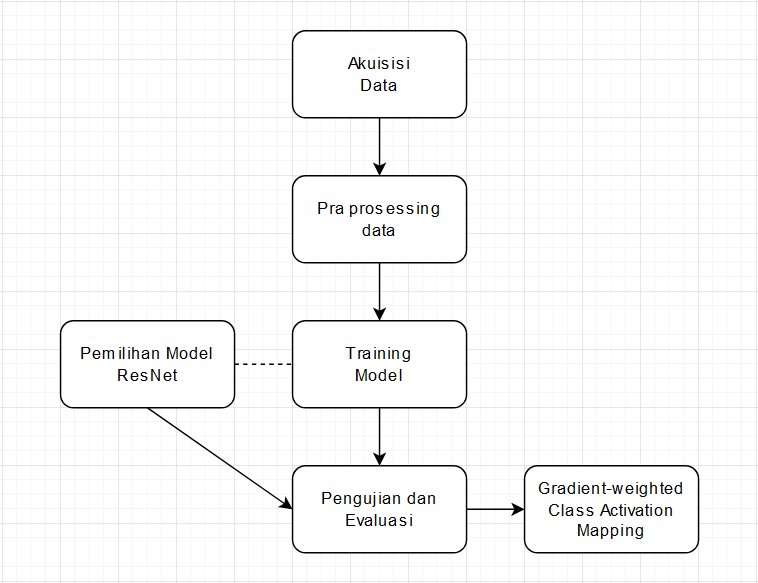
\includegraphics[scale=0.75]{gambar/diagramMethod.png}
	\caption{Diagram blok metodologi}
	\label{fig:diagramMethod}
\end{figure}

\section{Data dan Peralatan}
\label{sec:31}

\subsection{Dataset}
\label{sec:311}
Data yang digunakan dalam penelitian ini adalah data yang diperoleh dari Diabetic Retinopathy Analisis Grand challenge \parencite{drac_challenge_2023_10280359}, berupa citra OCT-\emph{Angiography}.
Untuk persebaran data yang digunakan pada penelitian ini, terdapat pada tabel \ref{table:Datasettraining}

Gambar yang diberikan adalah foto fundus retina yang digunakan untuk evaluasi retinopati diabetik, yang sudah diberi label berupa tingkat keparahan penyakit retinopati diabetik dan sebelumnya sudah melalui proses image assesment sehingga sudah siap digunakan untuk training model.
Foto ini menunjukkan detail dari jaringan pembuluh darah retina, disk optik, dan area makula. Berikut adalah deskripsi rinci dari gambar tersebut:

	\begin{figure}[H]
		\centering
		\subfloat[\centering Non-DR]{{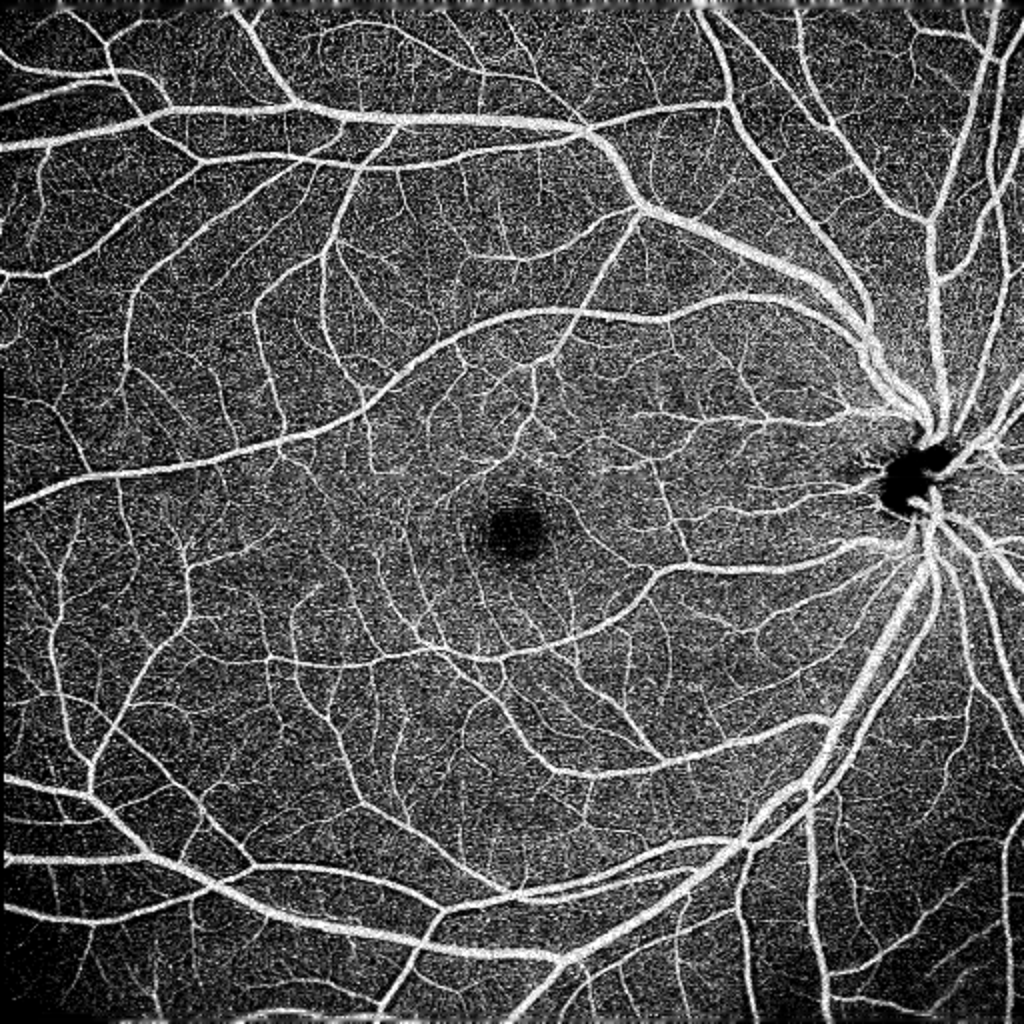
\includegraphics[width=5cm]{gambar/non-DR.png} }}%
		\subfloat[\centering NPDR]{{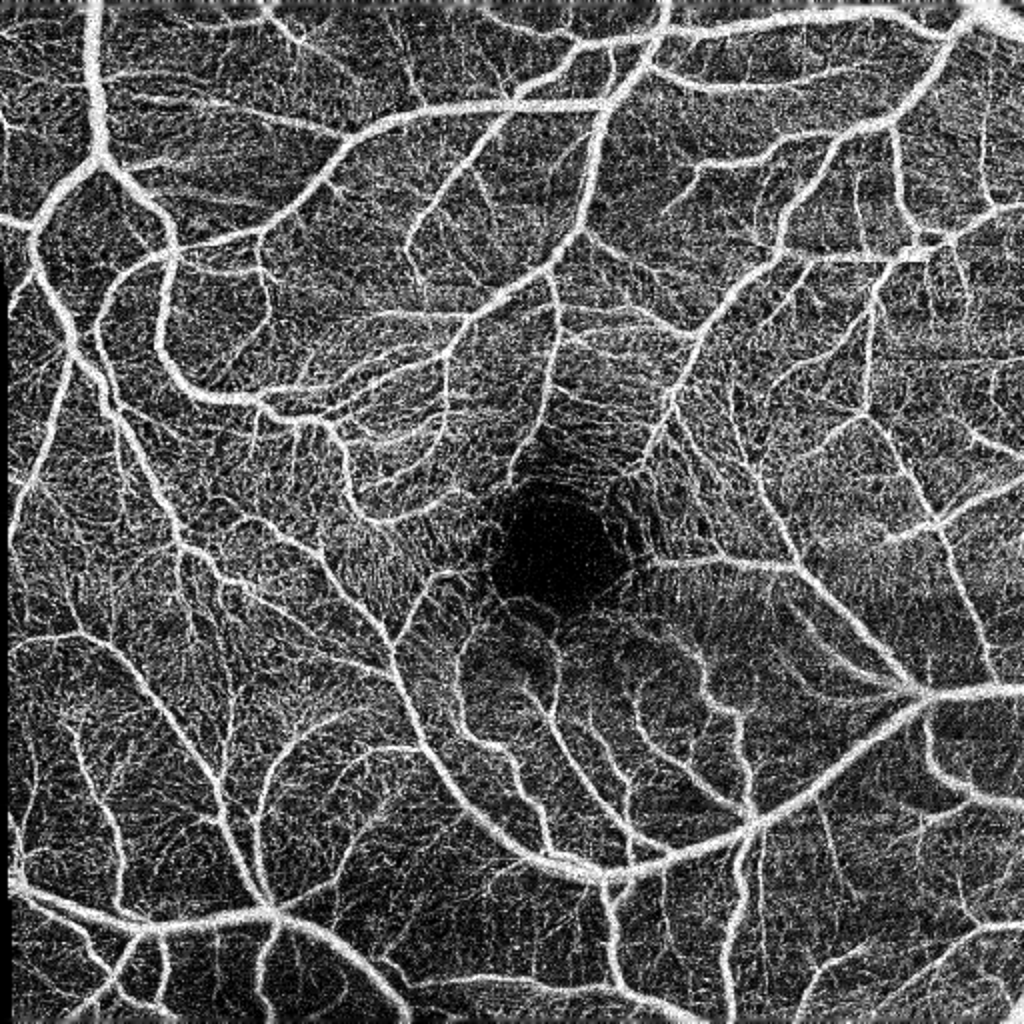
\includegraphics[width=5cm]{gambar/NPDR.png} }}%
		\subfloat[\centering PDR]{{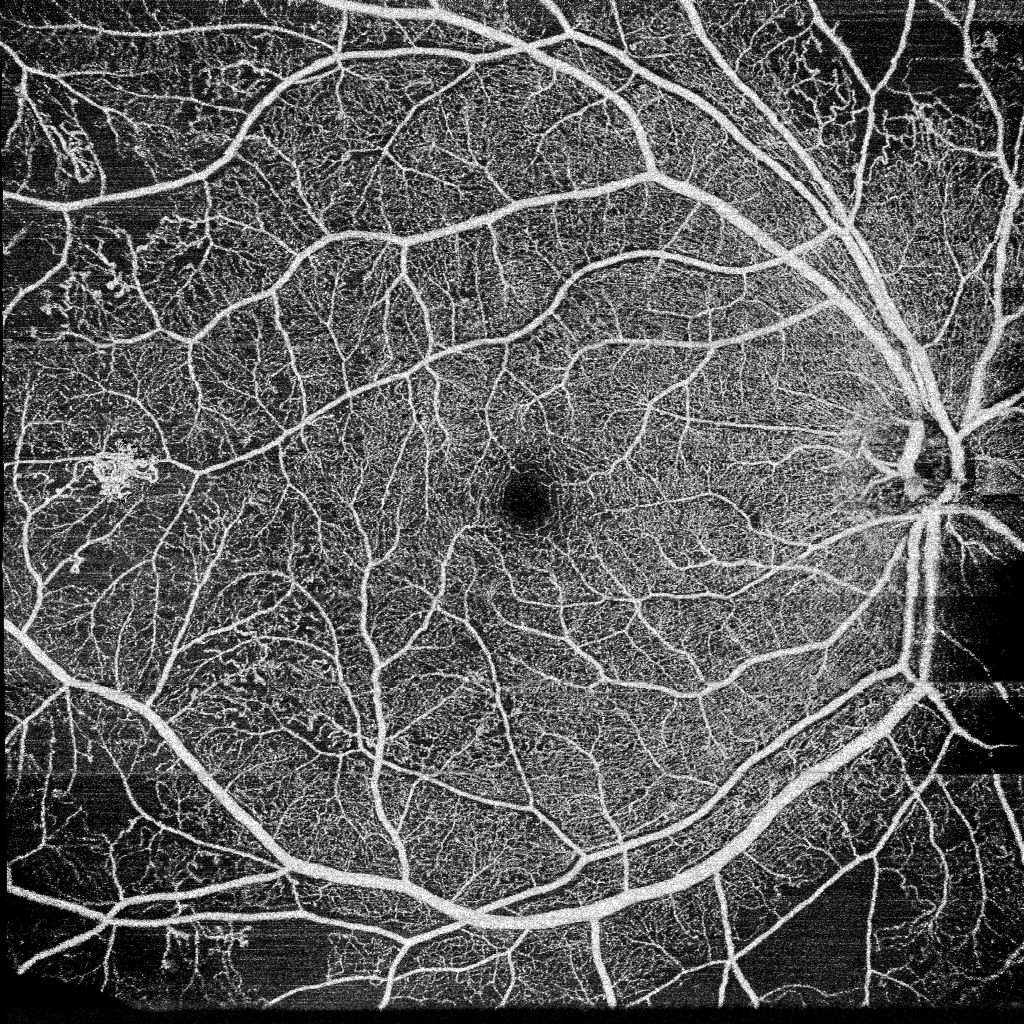
\includegraphics[width=5cm]{gambar/PDR.png} }}%
		\caption{Contoh Data Citra Retina}
		\label{fig:sampleDataset}
	\end{figure}

	\begin{itemize}
		\item \textbf{Struktur Vaskular}: Jaringan pembuluh darah yang jelas terlihat memancar dari disk optik. Pembuluh darah tampak menonjol dan tersebar di seluruh retina.
		\item \textbf{Makula}: Terdapat titik gelap yang terlihat di dekat makula, yang mungkin menunjukkan perubahan retina.
	\end{itemize}
Retinopati diabetik dapat dikategorikan berdasarkan tingkat keparahannya sebagai berikut:

	\begin{enumerate}
		\item Non-DR (0): Non-Diabetic Retinopathy

		\textbf{Karakteristik}: Tidak ada tanda-tanda retinopati diabetik. Retina tampak normal tanpa mikroaneurisma, pendarahan, atau eksudat keras.
		\item NPDR (1): Non-Proliferative Diabetic Retinopathy.

		\textbf{Karakteristik}:
		\begin{itemize}
			\item Kehadiran mikroaneurisma (lesi kecil bulat).\
			\item Pendarahan retina (bercak gelap kecil).
			\item Eksudat keras (bintik-bintik putih terang).
			\item Tidak ada neovaskularisasi.
		\end{itemize}
		\item PDR (2): Proliferative Diabetic Retinopathy

		\textbf{Karakteristik}:
		\begin{itemize}
			\item Kehadiran neovaskularisasi (pertumbuhan pembuluh darah baru yang abnormal).
			\item Mungkin ada pendarahan vitreous (ke dalam humor vitreous mata).
			\item Menunjukkan kondisi yang lebih parah dan berisiko tinggi terhadap kehilangan penglihatan.
		\end{itemize}
	\end{enumerate}

Informasi Dataset dari Tantangan DRAC
Dataset yang digunakan untuk pelatihan dan pengujian terdiri dari:

	\begin{itemize}
		\item Set Pelatihan: 611 gambar
		\item Set Uji: 386 gambar
	\end{itemize}
Gambar-gambar pada set pelatihan, kemudian dipisah kembali menjadi dua set, yaitu set untuk pelatihan dan set untuk validasi dengan jumlah sesuai pada tabel \ref{table:Datasettraining}

\begin{table}[hbtp]
	\begin{center}
	\caption{Tabel distribusi Set untuk Pelatihan dan Validasi}
	\label{table:Datasettraining}
	\begin{tabular}{|l|l|l|l|}
		\hline
		\rowcolor[HTML]{C0C0C0} 
		Label                                                & Klasifikasi & Jumlah & Total                                         \\ \hline
		\rowcolor[HTML]{FFFFFF} 
		\cellcolor[HTML]{FFFFFF}                             & non-DR      & 263    & \cellcolor[HTML]{FFFFFF}                      \\ \cline{2-3}
		\rowcolor[HTML]{FFFFFF} 
		\cellcolor[HTML]{FFFFFF}                             & NPDR        & 169    & \cellcolor[HTML]{FFFFFF}                      \\ \cline{2-3}
		\rowcolor[HTML]{FFFFFF} 
		\multirow{-3}{*}{\cellcolor[HTML]{FFFFFF}Training}   & PDR         & 56     & \multirow{-3}{*}{\cellcolor[HTML]{FFFFFF}488} \\ \hline
		\rowcolor[HTML]{FFFFFF} 
		\cellcolor[HTML]{FFFFFF}                             & non-DR      & 66     & \cellcolor[HTML]{FFFFFF}                      \\ \cline{2-3}
		\rowcolor[HTML]{FFFFFF} 
		\cellcolor[HTML]{FFFFFF}                             & NPDR        & 43     & \cellcolor[HTML]{FFFFFF}                      \\ \cline{2-3}
		\rowcolor[HTML]{FFFFFF} 
		\multirow{-3}{*}{\cellcolor[HTML]{FFFFFF}Validation} & PDR         & 14     & \multirow{-3}{*}{\cellcolor[HTML]{FFFFFF}123} \\ \hline
		\end{tabular}
	\end{center}
\end{table}

Sedangkan gambar pada set uji digunakan untuk mendapatkan penilaian online menggunakan metrik Quadratic Weighted Kappa dengan model dari DRAC sebagai pembandingnya. dan dikarenakan set uji yang diberikan ini tidak memiliki label, maka set ini tidak dapat dipergunakan untuk pengambilan metrik lain seperti \emph{precision, recall}, dan \emph{F1-score}.

\subsection{Peralatan}
\label{sec:312}

Dalam penelitian ini, penulis menggunakan komputer dengan sistem operasi Windows 11 dengan spesifikasi sebagai berikut:

\begin{itemize}
	\item Processor: Intel Core i5 12400F
	\item RAM: 16GB 3200MHz
	\item GPU: NVIDIA GeForce RTX 3060 Ti
	\subitem CUDA Cores: 4864
	\subitem Memory Config: 8 GB GDDR6
\end{itemize}

\subsection{Software}
\label{sec:313}

Software yang digunakan dalam penelitian ini adalah sebagai berikut:
\begin{itemize}
	\item Jupyter Notebook
	\item Visual Studio Code
\end{itemize}

\section{Metode yang Digunakan}
\label{sec:32}

\subsection{Skenario yang digunakan untuk peningkatan performa pelatihan model ResNet}
Dalam penelitian ini, dikarenakan oleh dataset yang sedikit dan terdapat \emph{class} yang kurang representatif, dilakukan metode berikut untuk penyeimbangan dataset.
\begin{itemize}
	\item Default

	Tidak ada Tindakan yang dilakukan untuk menyeimbangkan dataset. Metode ini dilakukan untuk variabel kontrol
	\item Penyesuaian \emph{Class-weight}

	Pada metode ini, dilakukan penambahan weight agar class yang underrepresented memiliki beban lebih tinggi
\end{itemize}

%\subsection{Akuisisi Data}
%\label{sec:321}
%Data yang digunakan dalam penelitian ini adalah data yang diperoleh dari Diabetic Retinopathy Analisis Grand challenge \parencite{drac_challenge_2023_10280359}. Data yang digunakan adalah data citra retina yang sudah diberi label berupa tingkat keparahan penyakit retinopati diabetik yang sebelumnya sudah melalui proses image assesment sehingga sudah siap digunakan untuk training model. Dataset ini berisikan 611 citra OCT-A yang telah diberi label. Dataset ini juga berisikan 386 citra OCT-A yang tidak berlabel untuk dijadikan testing dataset.

\subsection{Pra-pemrosesan Data}
\label{sec:322}
Pra-pemrosesan data dilakukan untuk mempersiapkan data sebelum dilakukan proses pelatihan model. Pra-pemrosesan data yang dilakukan adalah konversi citra retina dari format .jpeg menjadi .png. Hal ini dilakukan karena format .png memiliki ukuran yang lebih kecil dibandingkan dengan format .jpeg. Selain itu, format .png juga tidak mengurangi kualitas citra retina. Pra-pemrosesan data juga dilakukan untuk membagi data menjadi data latih dan data uji. Data latih digunakan untuk melatih model sedangkan data uji digunakan untuk menguji model.

\subsection{Model ResNet}
\label{sec:323}
Model ResNet yang akan digunakan untuk dibandingkan dalam penelitian ini adalah model pre-trained resnet-18, resnet-34, resnet-50, resnet-101, dan resnet-152. Performa model-model tersebut akan disajikan data dari nilai akurasi, \emph{loss}, dan \emph{val\_loss}. 

Dari setiap model yang telah dilatih, akan diambil tiga model, yaitu model dengan nilai akurasi \emph{training} terbaik (\emph{best trained}), nilai akurasi validasi terbaik (\emph{best validated}), serta model epoch terakhir yang dilatih (\emph{last trained}). Tiga model ini kemudian akan dievaluasi tersendiri, dan dibandingkan antara model yang dilatih tanpa menggunakan penyesuaian beban \emph{class}, dan model yang menggunakan penyesuaian beban \emph{class}.

\subsection{Pelatihan Model}
\label{sec:325}
Pelatihan model dilakukan dengan menggunakan metode \emph{transfer learning}. Metode \emph{transfer learning} dilakukan dengan menggunakan model ResNet yang sudah dipilih dan sudah dilatih dengan dataset ImageNet.
Arsitektur model yang digunakan sesuai pada penjelasan bagian \ref{sec:323} dengan menggunakan \emph{hyper-parameter} yang ada pada tabel \ref{tb:hyperParameterTraining}
\begin{table}[hbtp]
	\begin{center}
		\caption{Hyperparameter}
		\label{tb:hyperParameterTraining}
		\begin{tabular}{|
		>{\columncolor[HTML]{C0C0C0}}l |l|lll}
		\cline{1-2}
		Input shape                                         & 224,224,3      &  &  &  \\ \cline{1-2}
		Opimizer                                            & Adam           &  &  &  \\ \cline{1-2}
		Loss Function                                       & Cross Entropy  &  &  &  \\ \cline{1-2}
		Learning Rate                                       & 0.1            &  &  &  \\ \cline{1-2}
		Momentum                                            & 0.9            &  &  &  \\ \cline{1-2}
		\cellcolor[HTML]{C0C0C0}                            & Step size = 10 &  &  &  \\ \cline{2-2}
		\multirow{-2}{*}{\cellcolor[HTML]{C0C0C0}Scheduler} & Gamma = 0.1    &  &  &  \\ \cline{1-2}
		Epoch                                               & 100            &  &  &  \\ \cline{1-2}
		Batch size                                          & 32             &  &  &  \\ \cline{1-2}
		\end{tabular}
	\end{center}
\end{table}

\emph{Input shape} didapatkan dari model pre-training yang dilakukan berdasarkan yang digunakan pada original publishing ResNet \parencite{ResNet}, yaitu 224,224. Jadi, ukuran ini sudah menjadi yang tercanggih. Sehingga ketika dilakukan fine-tuning akan bagus karena konsisten dengan model sebelumnya.

Optimizer ADAM dipilih, karena ADAM dapat dibilang sebagai \emph{optimizer default} dan tidak perlu menghitung optimizer.

Cross Entropy digunakan karena kita melakukan klasifikasi \emph{multiclass} dalam proyek ini. Jadi, cross entropy digunakan untuk menghitung \emph{loss} dari model.

Learning rate \& scheduler

Setelah menghitung \emph{loss}, model akan mengetahui seberapa salahnya. Setelah itu dia akan melakukan backpropagation atau backtracking untuk mengupdate nilai baru setiap node neuron. Tidak ada acuan untuk nilai learning rate dan scheduler. Nilai diambil dari \emph{paper} yang ada, agar tetap konsisten. Dalam penerapannya, nilai ini akan dikalikan dengan turunan \emph{loss} sebagai learning rate. Dan model tersebut ingin mencapai titik terbaik di mana Adam membantu kita mencapai titik terbawah atau terendah dari fungsi tersebut.

Ukuran batch biasanya berhubungan dengan memori. Karena menggabungkan paket kumpulan data menjadi satu, lebih efisien karena satu epoch dapat mempelajari lebih banyak, tetapi membutuhkan lebih banyak memori. Misalnya, ukuran batch 32 berarti begitu memasuki jaringan saraf, akan ada paket data sebanyak 32 gambar.

Momentum dipilih berdasarkan \emph{paper} ResNet \parencite{ResNet}, yang mana dijelaskan betapa mulusnya saat menuruni bukit, yang ada hubungannya dengan optimalisasi \emph{learning rate}.


\subsection{Pengujian dan Evaluasi}
\label{sec:326}
Pengujian dan evaluasi dilakukan dengan menggunakan data uji. Pengujian dan evaluasi dilakukan dengan melihat nilai akurasi, \emph{loss}, dan \emph{val\_loss}. Selain itu, pengujian dan evaluasi juga dilakukan dengan melihat \emph{confusion matrix} dari model yang sudah dilatih, untuk dilihat nilai presisi, recall, dan F1 pada setiap kelasnya, untuk melihat performa model dalam memprediksi tingkat keparahan penyakit retinopati diabetik.

\subsection{Quadratic Weighted Kappa}
Dikarenakan dataset yang digunakan sangatlah kecil, maka metrik QWK juga digunakan untuk menghitung performa dari model. QWK dari model dihitung secara otomatis oleh sistem \emph{online grading} pada website Diabetic Retinopathy Grand Challenge (DRAC) \parencite{drac_challenge_2023_10280359}. Yang mana model yang dihasilkan dari pelatihan pada penelitian ini akan dihitung kesepakatannya dengan model yang ada pada sistem grading DRAC.

Metode grading menggunakan dataset \emph{testing} yang tidak berlabel. Model dari penelitian ini akan memprediksi:
\begin{itemize}
	\item Kelas yang diprediksi
	\item Nilai tensor untuk masing masing kelas (P0, P1, P2)
\end{itemize}
Dari setiap gambar pada dataset \emph{testing}. Hasil prediksi dikeluarkan dalam format .csv, kemudian diunggah ke website dari DRAC.
Setelah itu, sistem akan mengukur hasil QWK dari prediksi yang telah diunggah. Unggahan untuk penilaian terbatas lima kali dalam 24 jam.

\subsection{Gradient-weighted Class Activation Mapping}
\label{sec:327}
Grad-CAM digunakan untuk mengetahui faktor-faktor yang mempengaruhi model dalam memprediksi tingkat keparahan penyakit retinopati diabetik. Grad-CAM bekerja dengan menghitung gradien output model terhadap input, dan kemudian menggunakan gradien tersebut untuk memprediksi area input yang paling berkontribusi pada output model.

%Penelitian ini menggunakan pendekatan sistematis untuk mengkategorikan Non-DR (0), NPDR (1), dan PDR (2) menggunakan Grad-CAM dengan model ResNet-18 default, ResNet-18 class-wegihted, dan ResNet-152 yang telah dilatih sebelumnya. Prosesnya dimulai dengan persiapan model, yang memerlukan adaptasi jaringan saraf ResNet yang sudah ada untuk memenuhi tugas spesifik klasifikasi retinopati diabetik. Model ResNet, yang awalnya dilatih di ImageNet, disesuaikan dengan mengganti lapisan akhir yang terhubung sepenuhnya untuk mengakomodasi tiga kelas yang sesuai dengan berbagai tahap retinopati diabetik. Modifikasi ini memungkinkan jaringan untuk memanfaatkan fitur yang sudah ada sambil berfokus pada kategorisasi gambar retina ke dalam klasifikasi yang diinginkan. Selanjutnya, semua lapisan kecuali lapisan konvolusi terakhir dan lapisan terakhir yang terhubung sepenuhnya dibekukan untuk mempertahankan fitur yang diperoleh, yang merupakan aspek penting untuk klasifikasi yang tepat.
%
%Langkah selanjutnya melibatkan persiapan kumpulan data untuk penilaian. Citra retina menjalani berbagai langkah prapemrosesan seperti konversi ke hitam putih, pengubahan ukuran ke ukuran standar 224x224 pixel, normalisasi, dan konversi ke format tensor. Modifikasi ini memastikan bahwa gambar berada dalam format yang sesuai untuk dimasukkan ke dalam jaringan saraf. Kelas kumpulan data khusus dibuat untuk memfasilitasi pemuatan gambar dari direktori khusus yang mewakili kelas berbeda (Non-DR, NPDR, PDR). Dengan menyusun data dengan cara ini, proses pemuatan data selanjutnya menjadi lebih efektif, memungkinkan pemrosesan batch gambar secara efisien selama evaluasi. Pengaturan ini menjamin bahwa model menerima masukan yang konsisten dan terstandarisasi, yang sangat penting untuk memperoleh hasil klasifikasi yang dapat diandalkan.
%
%Setelah persiapan model dan data, Grad-CAM digunakan untuk membuat interpretasi visual untuk prediksi model. Grad-CAM adalah metode efektif yang mengidentifikasi wilayah tertentu dalam gambar masukan yang berdampak signifikan pada hasil klasifikasi model. Dengan berkonsentrasi pada lapisan konvolusional akhir model ResNet, Grad-CAM menghasilkan heatmap yang mengilustrasikan area gambar retina yang dianggap penting oleh model untuk membedakan antara Non-DR, NPDR, dan PDR. Peta panas ini kemudian ditumpangkan pada gambar asli, sehingga memberikan gambaran visual yang membantu memahami proses pengambilan keputusan model.
%
%Dalam penerapan Grad-CAM, model ResNet yang diadaptasi diinisialisasi dan dialihkan ke mode evaluasi. Grad-CAM secara khusus diarahkan pada lapisan konvolusional akhir model, sebuah langkah penting dalam menghasilkan interpretasi visual yang informatif. Melalui pengaturan ini, gambar masukan diproses untuk menghasilkan heatmap skala abu-abu yang menekankan area signifikan dalam gambar. Peta panas ini dilapiskan ke gambar retina asli untuk menciptakan visualisasi yang menampilkan titik fokus secara efektif. Alat bantu visual tersebut memainkan peran penting dalam memahami dan mengonfirmasi prediksi model, khususnya dalam skenario medis yang memerlukan interpretasi akurat.
%
%Visualisasi ini bertujuan untuk meningkatkan pemahaman prediksi model. Dengan merepresentasikan secara visual elemen gambar retina yang mempengaruhi klasifikasi Non-DR, NPDR, atau PDR, praktisi medis dapat memperoleh wawasan tentang karakteristik mendasar yang membedakan berbagai tahapan retinopati diabetik. Pendekatan metodologis ini tidak hanya meningkatkan transparansi model pembelajaran mendalam namun juga meningkatkan kegunaan praktisnya dalam situasi klinis, di mana alat bantu diagnostik yang dapat diandalkan dan dipahami sangat penting. 
Untuk melakukan klasifikasi Non-DR, NPDR, dan PDR menggunakan Grad-CAM dengan model ResNet-152 yang telah dilatih sebelumnya, dilakukan langkah-langkah berikut:

\subsubsection{Langkah 1: Persiapan Model}
Pertama, model jaringan saraf tiruan dibuat dengan memodifikasi ResNet-152 yang telah dilatih sebelumnya. 
Model ResNet-152 dimuat dengan bobot yang telah dilatih sebelumnya, dan lapisan akhir yang terhubung sepenuhnya disesuaikan untuk menghasilkan tiga kelas, sesuai dengan Non-DR (0), NPDR (1), dan PDR (2). 
Hal ini dilakukan dengan mengatur parameter num\_classes ke 3. 
Semua lapisan kecuali lapisan konvolusi terakhir (layer4) dan lapisan terakhir yang terhubung sepenuhnya dibekukan untuk mempertahankan fitur yang dipelajari dari ImageNet sambil memungkinkan lapisan terakhir beradaptasi dengan tugas klasifikasi retinopati diabetik spesifik. 

\begin{lstlisting}[
	label={lst:gradcam}
  ]
  Buat class DiabeticRetinopathyModel:
  Inisialisasi method class:
	  Muat model ResNet yang telah dilatih sebelumnya
	  Dapatkan jumlah fitur dari lapisan terakhir yang terhubung sepenuhnya
	  Ganti lapisan terakhir yang terhubung sepenuhnya dengan lapisan baru yang memiliki num_classes output
	  Bekukan semua lapisan kecuali lapisan konvolusi terakhir (layer4) dan lapisan terakhir yang terhubung sepenuhnya

  Method forward:
	  Lewatkan input x melalui model ResNet
	  Return output
\end{lstlisting}
%  class DiabeticRetinopathyModel(nn.Module):
%    def __init__(self, num_classes=3):
%        super(DiabeticRetinopathyModel, self).__init__()
%        self.resnet = resnet152(weights=ResNet152_Weights.IMAGENET1K_V2)
%        num_ftrs = self.resnet.fc.in_features
%        self.resnet.fc = nn.Linear(num_ftrs, num_classes)
%        for name, param in self.resnet.named_parameters():
%            if 'layer4' not in name:
%                param.requires_grad = False
%        self.resnet.fc.requires_grad = True
%
%    def forward(self, x):
%        return self.resnet(x)

\subsubsection{Langkah 2: Persiapan Data}
Untuk mempersiapkan dataset untuk evaluasi, gambar diproses dan diubah. 
Hal ini melibatkan pengubahan gambar menjadi skala abu-abu, mengubah ukurannya menjadi 224x224 piksel, menormalkannya, dan mengonversinya menjadi tensor. 
Kelas kumpulan data khusus dibuat untuk memuat gambar dari direktori masing-masing untuk setiap kelas (Non-DR, NPDR, PDR). 
Pemuat data kemudian di-instansiasi untuk memfasilitasi pemrosesan batch gambar selama evaluasi.

\begin{lstlisting}[
	%language=python,
	%caption={}
	label={lst:gradcamstep2}
]
Definisikan transformasi untuk gambar uji:
    Ubah gambar menjadi skala abu-abu dengan 3 output channels
    Ubah ukuran gambar menjadi 224x224 piksel
    Ubah gambar menjadi format tensor
    Normalisasi gambar dengan mean dan standar deviasi 0.5 untuk setiap channel

Kelas DiabeticRetinopathyTestDataset:
    Method __init__(img_dir, transform):
        Tetapkan direktori gambar dan transformasi
        Daftar semua nama file gambar di direktori

    Method __len__:
        Kembalikan jumlah gambar

    Method __getitem__(idx):
        Dapatkan nama file gambar pada indeks
        Muat gambar dari direktori
        Terapkan transformasi pada gambar (jika ada)
        Kembalikan gambar yang telah ditransformasi dan nama filenya

Buat instance dataset untuk setiap kelas:
    Muat gambar dari direktori "dataset/0" dengan transformasi yang telah didefinisikan
    Muat gambar dari direktori "dataset/1" dengan transformasi yang telah didefinisikan
    Muat gambar dari direktori "dataset/2" dengan transformasi yang telah didefinisikan

Buat data loader untuk setiap dataset dengan ukuran batch 1 dan tanpa pengacakan
\end{lstlisting}
%test_transform = transforms.Compose([
%    transforms.Grayscale(num_output_channels=3),
%    transforms.Resize((224, 224)),
%    transforms.ToTensor(),
%    transforms.Normalize(mean=[0.5, 0.5, 0.5], std=[0.5, 0.5, 0.5])
%])
%	class DiabeticRetinopathyTestDataset(Dataset):
%	    def __init__(self, img_dir, transform=None):
%	        self.img_dir = img_dir
%	        self.transform = transform
%	        self.img_list = os.listdir(img_dir)
%
%	    def __len__(self):
%	        return len(self.img_list)
%
%	    def __getitem__(self, idx):
%	        img_filename = self.img_list[idx]
%	        img_path = os.path.join(self.img_dir, img_filename)
%	        image = Image.open(img_path)
%	        if self.transform:
%	            image = self.transform(image)
%	        return image, img_filename
%
%	img_dir_0 = "dataset/0"
%	img_dir_1 = "dataset/1"
%	img_dir_2 = "dataset/2"
%	test_data_0 = DiabeticRetinopathyTestDataset(img_dir_0, test_transform)
%	test_data_1 = DiabeticRetinopathyTestDataset(img_dir_1, test_transform)
%	test_data_2 = DiabeticRetinopathyTestDataset(img_dir_2, test_transform)
%	test_dataloader_0 = DataLoader(test_data_0, batch_size=1, shuffle=False)
%	test_dataloader_1 = DataLoader(test_data_1, batch_size=1, shuffle=False)
%	test_dataloader_2 = DataLoader(test_data_2, batch_size=1, shuffle=False)

\subsubsection{Langkah 3: Menghasilkan Visualisasi Grad-CAM}
Grad-CAM digunakan untuk menghasilkan penjelasan visual untuk prediksi model. Model ResNet-152 yang telah dilatih sebelumnya, yang dimodifikasi untuk klasifikasi retinopati diabetik, dimuat dan diatur ke mode evaluasi. Grad-CAM diterapkan pada lapisan konvolusi terakhir untuk menyoroti daerah dalam gambar input yang penting untuk keputusan klasifikasi. Peta panas yang dihasilkan ditumpangkan pada gambar asli untuk memvisualisasikan area yang diminati.
\begin{lstlisting}[
	%language=python,
	%caption={}
	label={lst:gradcamstep3}
]
Impor library yang diperlukan untuk Grad-CAM dan pemrosesan gambar

Muat model ResNet yang telah dilatih dan dimodifikasi
Atur model ke mode evaluasi
Definisikan lapisan konvolusi terakhir (layer4) sebagai lapisan target untuk Grad-CAM

Inisialisasi Grad-CAM dengan model dan layer target

Tetapkan kelas target untuk visualisasi (misalnya, NPDR)

Hitung heatmap Grad-CAM untuk gambar input
Ekstrak heatmap

Overlay heatmap pada gambar asli untuk membuat visualisasi

\end{lstlisting}
%	from pytorch_grad_cam import GradCAM
%	from pytorch_grad_cam.utils.model_targets import ClassifierOutputTarget
%	from pytorch_grad_cam.utils.image import show_cam_on_image
%	import torch
%
%	model = torch.load("../resnet152val.pth")
%	model.eval()
%	target_layers = [model.resnet.layer4[-1]]
%
%	cam = GradCAM(model=model, target_layers=target_layers)
%
%	targets = [ClassifierOutputTarget(1)]
%	grayscale_cam = cam(input_tensor=image.unsqueeze(0), targets=targets)
%	grayscale_cam = grayscale_cam[0, :]
%	visualization = show_cam_on_image(image_real, grayscale_cam, use_rgb=False)
Dengan mengikuti langkah-langkah metodologi ini, model ini dapat mengklasifikasikan tahapan retinopati diabetik dan memberikan penjelasan visual untuk prediksinya, sehingga membantu dalam penafsiran dan kepercayaan terhadap hasil.
\cleardoublepage

% Bab 4 pengujian dan analisis
\chapter{HASIL DAN PEMBAHASAN}
\label{chap:4}

Pada penelitian ini dipaparkan hasil penelitian serta analisis dari model klasifikasi yang telah dibuat sesuai dengan desain sistem dan implementasi pada Bab 3. Data yang digunakan pada pengujian ini menggunakan dataset DRAC dengan data splitting yang telah dilakukan pra-pemrosesan sebelumnya.

Berikut adalah hasil yang didapatkan dari penelitian yang telah dilakukan:

\section{Hasil Penelitian}
\label{sec:41}

Metrik yang digunakan untuk menentukan performa dari model pada saat dilatih atau training adalah akurasi dan loss. Kedua metrik ini bertujuan untuk melihat kondisi model telah fit atau tidak yang dapat menyebabkan kesulitan dalam memprediksi data yang belum pernah dilihat oleh model tersebut.

Model yang digunakan pada proses pengujian ada tiga, yaitu model dengan nilai training accuracy tertinggi, model dengan nilai validasi tertinggi, dan model terakhir dalam pelatihan.

Evaluasi dari hasil penelitian ini dilakukan dengan menggunakan beberapa metriks lain yaitu precision, recall, dan F1-score. Metrik-metrik tersebut, digunakan untuk mengukur akurasi dari model yang telah dibuat.

\subsection{Hasil Pengujian Model tanpa menggunakan Penyesuaian}
\label{sec:411}

Untuk setiap model \emph{ResNet} yang digunakan akan dilakukan pelatihan sebanyak 100 epoch pada tiga kelas dataset berbeda, yaitu: \emph{non-diabetic retinopathy} (non-DR), \emph{proliferative diabetic retinopathy} (PDR), dan \emph{non-proliferative diabetic retinopathy} (NPDR).

Data akan diambil dari model dengan nilai training terbaik (\emph{best trained}), validasi terbaik (\emph{best validated}), serta model terakhir yang dilatih (\emph{last trained}).

Sebagai kontrol, dilakukan uji coba \emph{training} yang tidak menggunakan penyesuaian \emph{gradient-weighted class activation mapping} pada dataset sesuai pada bagian \ref{sec:32}. Uji coba ini dilakukan pada seluruh variasi model \emph{ResNet} yang digunakan dan sebagai metrik akan digunakan nilai akurasi, precision, recall, dan nilai F1.

Dikarenakan dataset yang dipakai cenderung kecil, dan data untuk testing tidak memiliki label, maka dilakukan satu parameter lain untuk penilaian, yaitu \emph{Quadratic Weighted Kappa} (QWK). Penilaian ini bertujuan untuk meninjau kesetujuan antara model yang didapatkan, dengan model yang ada pada challenge dari DRAC. Hasil pengujian metrik dapat dihilat lebih jelas pada Tabel 4.1, Tabel 4.2, dan Tabel 4.3

\pagebreak

\begin{table}[hbtp]
	\begin{center}
		\caption{Hasil Best Trained model}
		\label{tb:HasilTrainDefault}
		\begin{tabular}{|c|l|c|l|l|l|c|}
			\hline
			\rowcolor[HTML]{C0C0C0} 
			Arsitektur & \multicolumn{1}{c|}{\cellcolor[HTML]{C0C0C0}class} & acc                      & \multicolumn{1}{c|}{\cellcolor[HTML]{C0C0C0}prec} & \multicolumn{1}{c|}{\cellcolor[HTML]{C0C0C0}rec} & \multicolumn{1}{c|}{\cellcolor[HTML]{C0C0C0}F1} & QWK                                  \\ \hline
			& non-DR                                             &                          & 0,875                                             & 0,848485                                         & 0,861538                                        &                                      \\ \cline{2-2} \cline{4-6}
			& NPDR                                               &                          & 0,645833                                          & 0,72093                                          & 0,681319                                        &                                      \\ \cline{2-2} \cline{4-6}
			\multirow{-3}{*}{ResNet-18}  & PDR                                                & \multirow{-3}{*}{0,7642} & 0,636364                                          & 0,5                                              & 0,56                                            & \multirow{-3}{*}{\textbf{0.7583626695732866}} \\ \hline
			& non-DR                                             &                          & 0,83871                                           & 0,787879                                         & 0,8125                                          &                                      \\ \cline{2-2} \cline{4-6}
			& NPDR                                               &                          & 0,64                                              & 0,744186                                         & 0,688172                                        &                                      \\ \cline{2-2} \cline{4-6}
			\multirow{-3}{*}{ResNet-34}  & PDR                                                & \multirow{-3}{*}{0,748}  & 0,727273                                          & 0,571429                                         & 0,64                                            & \multirow{-3}{*}{0.7218079395196282} \\ \hline
			& non-DR                                             &                          & 0,863636                                          & 0,863636                                         & 0,863636                                        &                                      \\ \cline{2-2} \cline{4-6}
			& NPDR                                               &                          & \textbf{0,688889}                                          & 0,72093                                          & 0,704545                                        &                                      \\ \cline{2-2} \cline{4-6}
			\multirow{-3}{*}{ResNet-50}  & PDR                                                & \multirow{-3}{*}{0,7805} & 0,666667                                          & 0,571429                                         & 0,615385                                        & \multirow{-3}{*}{0.7266403960229424} \\ \hline
			& non-DR                                             &                          & 0,873016                                          & 0,833333                                         & 0,852713                                        &                                      \\ \cline{2-2} \cline{4-6}
			& NPDR                                               &                          & 0,673913                                          & 0,72093                                          & 0,696629                                        &                                      \\ \cline{2-2} \cline{4-6}
			\multirow{-3}{*}{ResNet-101} & PDR                                                & \multirow{-3}{*}{0,7805} & 0,714286                                          & \textbf{0,714286}                                         & \textbf{0,714286}                                        & \multirow{-3}{*}{0.7503614091151183} \\ \hline
			& non-DR                                             &                          & \textbf{0,878788}                                          & \textbf{0,878788}                                         & \textbf{0,878788}                                        &                                      \\ \cline{2-2} \cline{4-6}
			& NPDR                                               &                          & 0,68                                              & \textbf{0,790698}                                         & \textbf{0,731183}                                        &                                      \\ \cline{2-2} \cline{4-6}
			\multirow{-3}{*}{ResNet-152} & PDR                                                & \multirow{-3}{*}{\textbf{0,7967}} & \textbf{0,857143}                                          & 0,428571                                         & 0,571429                                        & \multirow{-3}{*}{0.6937048139657909} \\ \hline
		\end{tabular}
	\end{center}
\end{table}

Dari model dengan nilai training terbaik didapatkan nilai akurasi terbaik sebesar \textbf{0.7967} dari arsitektur \emph{ResNet-152}.

\begin{itemize}

\item Untuk dataset non-DR didapatkan nilai precision, recall, dan F1 sebesar \textbf{0.878788} dari arsitektur \emph{ResNet-152};

\item Untuk dataset NPDR didapatkan nilai precision sebesar \textbf{0.688889} dari arsitektur \emph{ResNet-50}, nilai recall sebesar \textbf{0.790698} dari arsitektur \emph{ResNet-152}, nilai F1 sebesar \textbf{0.731183} dari arsitektur \emph{ResNet-152};

\item Untuk dataset PDR didapatkan nilai precision sebesar \textbf{0.857143} dari arsitektur \emph{ResNet-152}, nilai recall sebesar \textbf{0.714286} dari arsitektur \emph{ResNet-101}, nilai F1 sebesar \textbf{0.714286} dari arsitektur \emph{ResNet-101}.

\end{itemize}

Dari seluruh arsitektur \emph{ResNet} yang digunakan, nilai QWK tertinggi sebesar \textbf{0.7583626695732866} didapatkan dari arsitektur \emph{ResNet-18}. Untuk hasil dari best validated model dari setiap arsitektur ResNet dapat dilihat pada tabel \ref{tb:HasilValDefault}

\pagebreak

\begin{table}[hbtp]
	\begin{center}
		\caption{Hasil Best Validated model}
		\label{tb:HasilValDefault}
		\begin{tabular}{|c|l|c|l|l|l|c|}
			\hline
			\rowcolor[HTML]{C0C0C0} 
			Arsitektur & \multicolumn{1}{c|}{\cellcolor[HTML]{C0C0C0}class} & acc                      & \multicolumn{1}{c|}{\cellcolor[HTML]{C0C0C0}prec} & \multicolumn{1}{c|}{\cellcolor[HTML]{C0C0C0}rec} & \multicolumn{1}{c|}{\cellcolor[HTML]{C0C0C0}F1} & QWK                                  \\ \hline
			& non-DR                                             &                          & 0,904762                                          & 0,863636                                         & 0,883721                                        &                                      \\ \cline{2-2} \cline{4-6}
			& NPDR                                               &                          & 0,698113                                          & 0,860465                                         & \textbf{0,770833}                               &                                      \\ \cline{2-2} \cline{4-6}
			\multirow{-3}{*}{ResNet-18}  & PDR                                                & \multirow{-3}{*}{0,8211} & 1                                                 & 0,5                                              & 0,666667                                        & \multirow{-3}{*}{0.7332556875533816} \\ \hline
			& non-DR                                             &                          & 0,818182                                          & \textbf{0,954545}                                & 0,881119                                        &                                      \\ \cline{2-2} \cline{4-6}
			& NPDR                                               &                          & \textbf{0,756757}                                 & 0,651163                                         & 0,7                                             &                                      \\ \cline{2-2} \cline{4-6}
			\multirow{-3}{*}{ResNet-34}  & PDR                                                & \multirow{-3}{*}{0,8049} & 0,888889                                          & \textbf{0,571429}                                & \textbf{0,695652}                                        & \multirow{-3}{*}{0.7074309213982319} \\ \hline
			& non-DR                                             &                          & 0,847222                                          & 0,924242                                         & 0,884058                                        &                                      \\ \cline{2-2} \cline{4-6}
			& NPDR                                               &                          & 0,714286                                          & 0,697674                                         & 0,705882                                        &                                      \\ \cline{2-2} \cline{4-6}
			\multirow{-3}{*}{ResNet-50}  & PDR                                                & \multirow{-3}{*}{0,7967} & 0,777778                                          & 0,5                                              & 0,608696                                        & \multirow{-3}{*}{0.7051400702187358} \\ \hline
			& non-DR                                             &                          & \textbf{0,931034}                                 & 0,818182                                         & 0,870968                                        &                                      \\ \cline{2-2} \cline{4-6}
			& NPDR                                               &                          & 0,666667                                          & \textbf{0,883721}                                & 0,76                                            &                                      \\ \cline{2-2} \cline{4-6}
			\multirow{-3}{*}{ResNet-101} & PDR                                                & \multirow{-3}{*}{0,8049} & 0,875                                             & 0,5                                              & 0,636364                                        & \multirow{-3}{*}{0.6899458931486075} \\ \hline
			& non-DR                                             &                          & 0,869565                                          & 0,909091                                         & \textbf{0,888889}                               &                                      \\ \cline{2-2} \cline{4-6}
			& NPDR                                               &                          & 0,717391                                          & 0,767442                                         & 0,741573                                        &                                      \\ \cline{2-2} \cline{4-6}
			\multirow{-3}{*}{ResNet-152} & PDR                                                & \multirow{-3}{*}{0,813}  & 0,875                                             & 0,5                                              & 0,636364                                        & \multirow{-3}{*}{0.7303200133655321} \\ \hline
		\end{tabular}
	\end{center}
\end{table}

Dari model terakhir yang telah dilatih, arsitektur \emph{ResNet-101} dan \emph{ResNet-34} mendapatkan nilai akurasi yang sama, yaitu sebesar \textbf{0.8049}.

\begin{itemize}
	
	\item Untuk dataset non-DR didapatkan nilai precision sebesar \textbf{0,931034} dari arsitektur \emph{ResNet-101}, recall sebesar \textbf{0,954545} dari arsitektur \emph{ResNet-34}, dan F1 sebesar \textbf{0,888889} dari arsitektur \emph{ResNet-152};
	
	\item Untuk dataset NPDR didapatkan nilai precision sebesar \textbf{0,756757} dari arsitektur \emph{ResNet-34}, nilai recall sebesar \textbf{0,883721} dari arsitektur \emph{ResNet-101}, nilai F1 sebesar \textbf{0,770833} dari arsitektur \emph{ResNet-18};
	
	\item Untuk dataset PDR didapatkan nilai precision sebesar \textbf{1} dari arsitektur \emph{ResNet-34}, nilai recall sebesar \textbf{0.571429} dari arsitektur \emph{ResNet-18}, nilai F1 sebesar \textbf{0,695652} dari arsitektur \emph{ResNet-34}.
	
\end{itemize}

Dari seluruh arsitektur \emph{ResNet} yang digunakan, nilai QWK tertinggi sebesar \textbf{0.7332556875533816} didapatkan dari arsitektur \emph{ResNet-18}. Untuk hasil dari model epoch terakhir dari setiap arsitektur ResNet dapat dilihat pada tabel \ref{tb:HasilLastDefault}
\pagebreak

\begin{table}[hbtp]
	\begin{center}
		\caption{Hasil Last trained model}
		\label{tb:HasilLastDefault}
		\begin{tabular}{|c|l|c|l|l|l|c|}
			\hline
			\rowcolor[HTML]{C0C0C0} 
			Arsitektur   & \multicolumn{1}{c|}{\cellcolor[HTML]{C0C0C0}class} & acc                      & \multicolumn{1}{c|}{\cellcolor[HTML]{C0C0C0}prec} & \multicolumn{1}{c|}{\cellcolor[HTML]{C0C0C0}rec} & \multicolumn{1}{c|}{\cellcolor[HTML]{C0C0C0}F1} & QWK                                  \\ \hline
			& non-DR                                             &                          & 0,861538                                          & 0,848485                                         & 0,854962                                        &                                      \\ \cline{2-2} \cline{4-6}
			& NPDR                                               &                          & 0,652174                                          & 0,697674                                         & 0,674157                                        &                                      \\ \cline{2-2} \cline{4-6}
			\multirow{-3}{*}{ResNet-18}  & PDR                                                & \multirow{-3}{*}{0,7642} & 0,666667                                          & \textbf{0,571429}                                         & \textbf{0,615385}                                        & \multirow{-3}{*}{\textbf{0.7543612091028568}} \\ \hline
			& non-DR                                             &                          & 0,857143                                          & 0,818182                                         & 0,837209                                        &                                      \\ \cline{2-2} \cline{4-6}
			& NPDR                                               &                          & 0,666667                                          & \textbf{0,790698}                                         & 0,723404                                        &                                      \\ \cline{2-2} \cline{4-6}
			\multirow{-3}{*}{ResNet-34}  & PDR                                                & \multirow{-3}{*}{0,7724} & \textbf{0,777778}                                          & 0,5                                              & 0,608696                                        & \multirow{-3}{*}{0.7289056625189767} \\ \hline
			& non-DR                                             &                          & 0,808824                                          & 0,833333                                         & 0,820896                                        &                                      \\ \cline{2-2} \cline{4-6}
			& NPDR                                               &                          & 0,581395                                          & 0,581395                                         & 0,581395                                        &                                      \\ \cline{2-2} \cline{4-6}
			\multirow{-3}{*}{ResNet-50}  & PDR                                                & \multirow{-3}{*}{0,6992} & 0,5                                               & 0,428571                                         & 0,461538                                        & \multirow{-3}{*}{0.7282307517601635} \\ \hline
			& non-DR                                             &                          & \textbf{0,909091}                                          & \textbf{0,909091}                                         & \textbf{0,909091}                                        &                                      \\ \cline{2-2} \cline{4-6}
			& NPDR                                               &                          & \textbf{0,711111}                                          & 0,744186                                         & \textbf{0,727273}                                        &                                      \\ \cline{2-2} \cline{4-6}
			\multirow{-3}{*}{ResNet-101} & PDR                                                & \multirow{-3}{*}{\textbf{0,8049}} & 0,583333                                          & 0,5                                              & 0,538462                                        & \multirow{-3}{*}{0.7417574983086521} \\ \hline
			& non-DR                                             &                          & 0,852459                                          & 0,787879                                         & 0,818898                                        &                                      \\ \cline{2-2} \cline{4-6}
			& NPDR                                               &                          & 0,603774                                          & 0,744186                                         & 0,666667                                        &                                      \\ \cline{2-2} \cline{4-6}
			\multirow{-3}{*}{ResNet-152} & PDR                                                & \multirow{-3}{*}{0,7398} & \textbf{0,777778}                                          & 0,5                                              & 0,608696                                        & \multirow{-3}{*}{0.6850781547845979} \\ \hline
		\end{tabular}
	\end{center}
\end{table}

Dari model terakhir yang telah dilatih, didapatkan nilai akurasi terbaik sebesar \textbf{0.8049} dari arsitektur \emph{ResNet-101}.

\begin{itemize}
	
	\item Untuk dataset non-DR didapatkan nilai precision, recall, dan F1 sebesar \textbf{0.909091} dari arsitektur \emph{ResNet-101};
	
	\item Untuk dataset NPDR didapatkan nilai precision sebesar \textbf{0.711111} dari arsitektur \emph{ResNet-101}, nilai recall sebesar \textbf{0.790698} dari arsitektur \emph{ResNet-34}, nilai F1 sebesar \textbf{0.727273} dari arsitektur \emph{ResNet-101};
	
	\item Untuk dataset PDR didapatkan nilai precision sebesar \textbf{0.777778} dari arsitektur \emph{ResNet-34} dan \emph{ResNet-152}, nilai recall sebesar \textbf{0.571429} dari arsitektur \emph{ResNet-18}, nilai F1 sebesar \textbf{0.615385} dari arsitektur \emph{ResNet-18}.
	
\end{itemize}

Dari seluruh arsitektur \emph{ResNet} yang digunakan, nilai QWK tertinggi sebesar \textbf{0.7543612091028568} didapatkan dari arsitektur \emph{ResNet-18}.

Grafik dari \emph{training loss}, \emph{training accuracy}, dan \emph{validation accuracy} pada setiap arsitektur yang tidak menggunakan penyesuaian \emph{class weight} dapat dilihat dengan lebih jelas pada Gambar \ref{Fig:GraphTrainingDefPt2} Nilai loss cukup tinggi pada permulaan dikarenakan ukuran \emph{batch} yang cukup kecil, sehingga jumlah training sample yang digunakan dalam satu batch untuk satu iterasi juga kecil. Namun, setelah epoch tertentu, model akan menjaga nilai loss-nya tetap stabil pada nilai yang relatif rendah.
\pagebreak
\begin{figure}[hbtp]
	\centering
	\subfloat[\centering Training Loss dan Akurasi ResNet-18]{{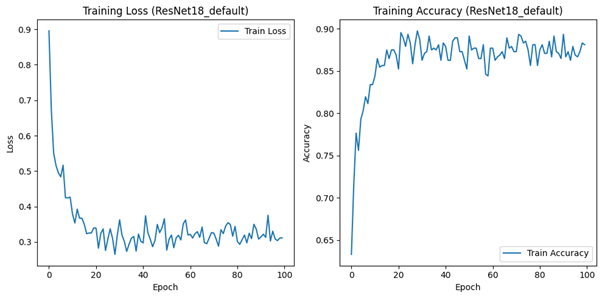
\includegraphics[height=7cm]{gambar/TrainingGraphResNet18.png}}}
	\qquad
	\subfloat[\centering Training Loss dan Akurasi ResNet-34]{{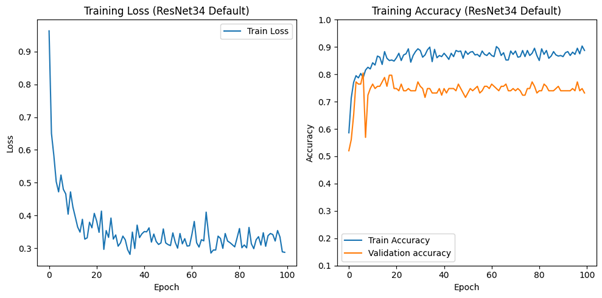
\includegraphics[height=7cm]{gambar/TrainingGraphResNet34.png}}}
	\caption{Grafik Training Loss dan akurasi ResNet-18 dan ResNet-34 Tanpa Penyesuaian Beban pada \emph{Class}}
	\label{Fig:GraphTrainingDefPt1}
\end{figure}

Dari grafik Training Loss dari \emph{ResNet-18 Default} dan \emph{ResNet-34 Default}  dapat dilihat bahwa nilai loss mulai dari \textbf{1.0}/mendekati \textbf{1.0} dan dengan cepat menjadi stabil mendekati epoch ke-\textbf{20} dengan nilai menjadi fluktuatif di antara \textbf{0.3 dan 0.4}.

Dari grafik Training Accuracy \emph{ResNet-18 Default} dapat dilihat bahwa akurasi training mulai dari nilai \textbf{0.6} dan dengan cepat menjadi stabil mendekati epoch ke-\textbf{10} dimana nilai berada di antara \textbf{0.8 dan 0.9} 

Dari grafik Training Accuracy \emph{ResNet-18 Default} dapat dilihat bahwa akurasi validasi mulai dari nilai \textbf{0.6} dan bersifat fluktuatif hingga epoch ke-\textbf{20} dimana nilai menjadi stabil di antara \textbf{0.7 dan 0.8}.

Dari grafik Training Accuracy \emph{ResNet-34 Default} dapat dilihat bahwa akurasi validasi mulai dari nilai \textbf{0.5} dan bersifat fluktuatif hingga sebelum epoch ke-\textbf{20} dimana nilai menjadi stabil di antara \textbf{0.7 dan 0.8}.

Untuk Grafik training ResNet-50 dan Resnet-101, dapat dilihat pada Gambar \ref{Fig:GraphTrainingDefPt2} di bawah ini.

\begin{figure}[hbtp]
	\centering
	\subfloat[\centering Training Loss dan Akurasi ResNet-50]{{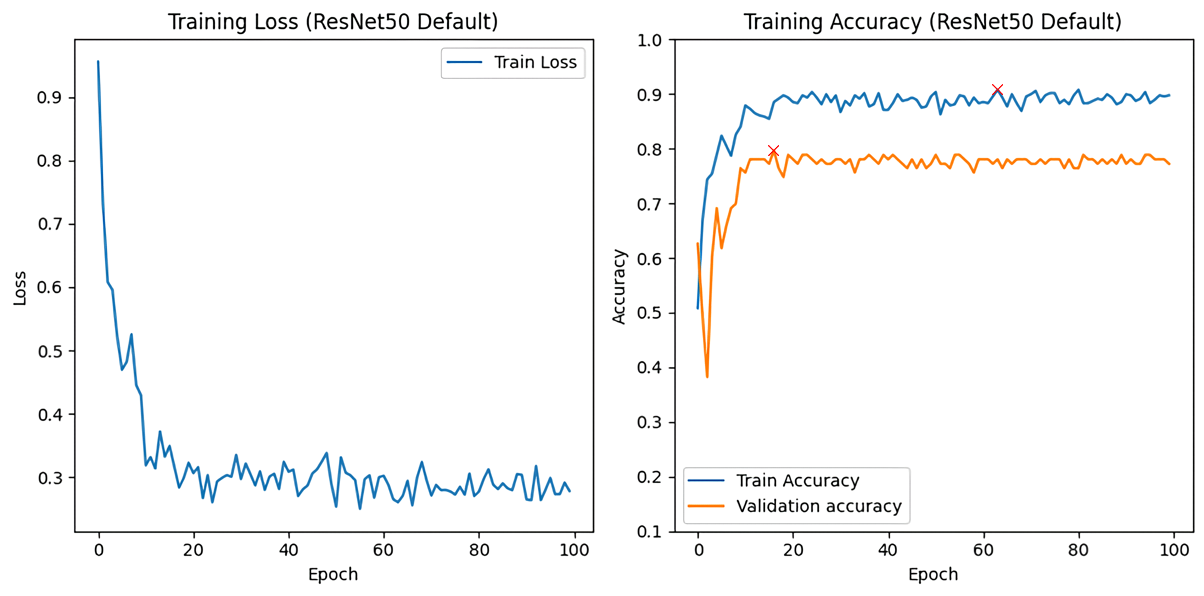
\includegraphics[height=7cm]{gambar/TrainingGraphResNet50.png}}}
	\qquad
	\subfloat[\centering Training Loss dan Akurasi ResNet-101]{{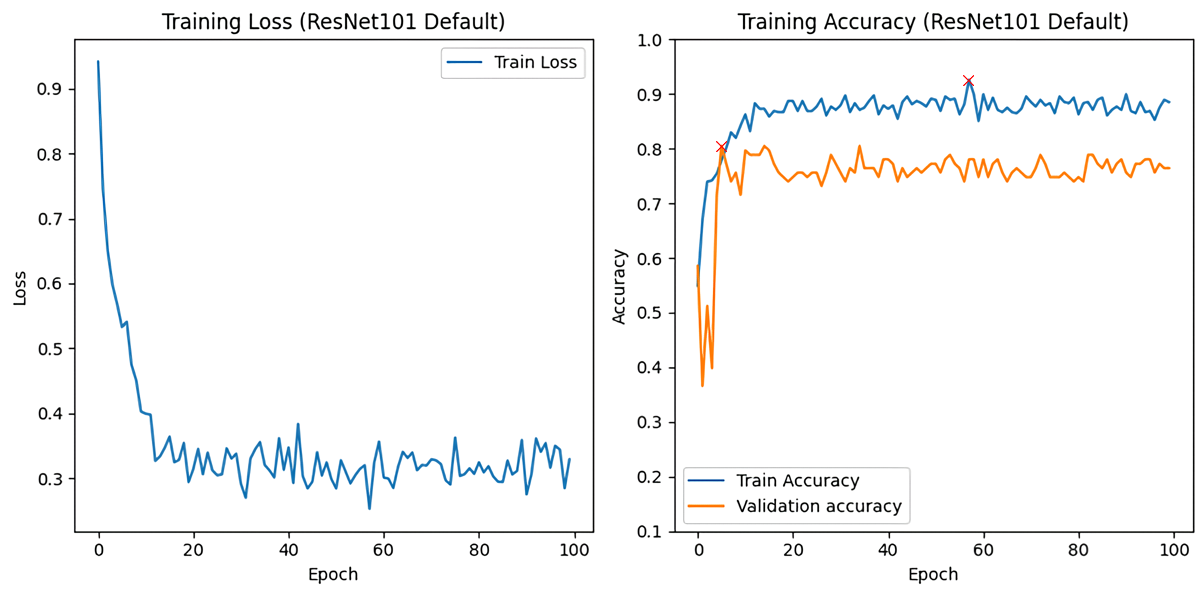
\includegraphics[height=7cm]{gambar/TrainingGraphResNet101.png}}}
	\caption{Grafik Training Loss dan akurasi ResNet-50 dan ResNet-101 Tanpa Penyesuaian Beban pada \emph{Class}}
	\label{Fig:GraphTrainingDefPt2}
\end{figure}
Dari grafik Training Loss \emph{ResNet-50 Default} dapat dilihat bahwa nilai loss mulai dari \textbf{1.0} dan dengan cepat menjadi stabil mendekati epoch ke-\textbf{20} dengan nilai menjadi fluktuatif di antara \textbf{0.3 dan 0.4}.

Dari grafik Training Accuracy \emph{ResNet-50 Default} dapat dilihat bahwa akurasi training mulai dari nilai \textbf{0.6} dan dengan cepat menjadi stabil mendekati epoch ke-\textbf{10} dimana nilai berada di antara \textbf{0.8 dan 0.9} 

Dari grafik Training Accuracy \emph{ResNet-50 Default} dapat dilihat bahwa akurasi validasi mulai dari nilai \textbf{0.6} dan bersifat fluktuatif hingga epoch ke-\textbf{20} dimana nilai menjadi stabil di antara \textbf{0.7 dan 0.8}.

Kemudian Dari grafik Training Loss \emph{ResNet-101 Default} dapat dilihat bahwa nilai loss mulai dari \textbf{1.0} dan dengan cepat menjadi stabil mendekati epoch ke-\textbf{20} dengan nilai menjadi fluktuatif di antara \textbf{0.3 dan 0.4}.

Dari grafik Training Accuracy \emph{ResNet-101 Default} dapat dilihat bahwa akurasi training mulai dari nilai \textbf{0.6} dan dengan cepat menjadi stabil mendekati epoch ke-\textbf{10} dimana nilai berada di antara \textbf{0.8 dan 0.9} 

Dari grafik Training Accuracy \emph{ResNet-101 Default} dapat dilihat bahwa akurasi validasi mulai dari nilai \textbf{0.6} dan bersifat fluktuatif hingga epoch ke-\textbf{20} dimana nilai menjadi stabil di antara \textbf{0.7 dan 0.8}.

\begin{figure}[hbtp]
	\subfloat[\centering Training Loss dan Akurasi ResNet-152]{{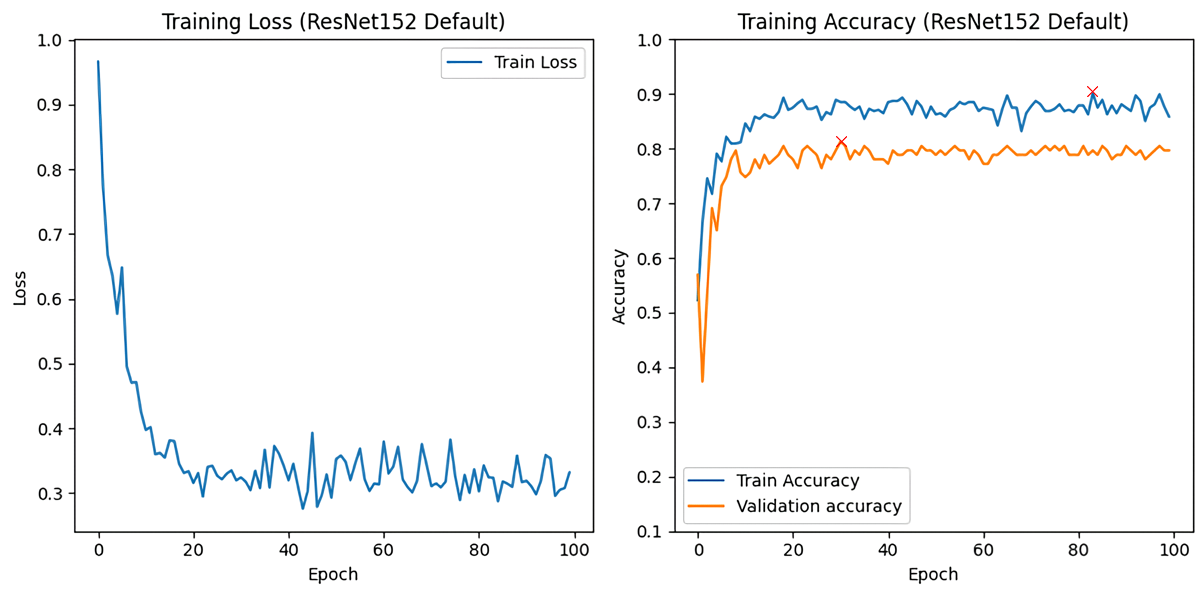
\includegraphics[height=7cm]{gambar/TrainingGraphResNet152.png}}}
	\caption{Grafik Training Loss dan akurasi ResNet-152 Tanpa Penyesuaian Beban pada \emph{Class}}
	\label{Fig:GraphTrainingDefPt3}
\end{figure}
Dari grafik Training Loss \emph{ResNet-152 Default} dapat dilihat bahwa nilai loss mulai dari \textbf{1.0} dan dengan cepat menjadi stabil mendekati epoch ke-\textbf{20} dengan nilai menjadi fluktuatif di antara \textbf{0.3 dan 0.4}.

Dari grafik Training Accuracy \emph{ResNet-152 Default} dapat dilihat bahwa akurasi training mulai dari nilai \textbf{0.6} dan dengan cepat menjadi stabil mendekati epoch ke-\textbf{10} dimana nilai berada di antara \textbf{0.8 dan 0.9} 

Dari grafik Training Accuracy \emph{ResNet-152 Default} dapat dilihat bahwa akurasi validasi mulai dari nilai \textbf{0.6} dan bersifat fluktuatif hingga epoch ke-\textbf{20} dimana nilai menjadi stabil di antara \textbf{0.7 dan 0.8}.

Untuk \emph{confusion matrix} dari setiap arsitektur dapat dilihat pada Gambar \ref{fig:confRes18}, Gambar \ref{fig:confRes34}, Gambar \ref{fig:confRes50}, Gambar \ref{fig:confRes101}, dan Gambar \ref{fig:confRes152}. Masing - masing gambar terdiri dari tiga \emph{confusion matrix}, yang masing - masing confusion matrix merupakan hasil dari model dengan akurasi \emph{training} terbaik, model dengan akurasi validasi terbaik, dan model terakhir dari 100 \emph{epoch} pada arsitektur tersebut.
\pagebreak
\begin{figure}[hbtp]
	\centering
	\subfloat[\centering Best Train acc ResNet-18]{{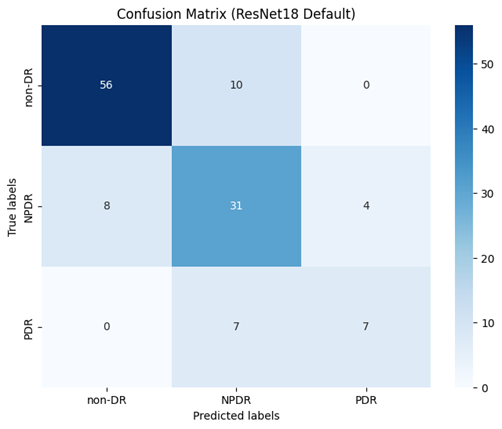
\includegraphics[width=7cm]{gambar/confusionMatrixResnet18_bestTrain.png} }}%
	\qquad
	\subfloat[\centering Best Val acc ResNet-18]{{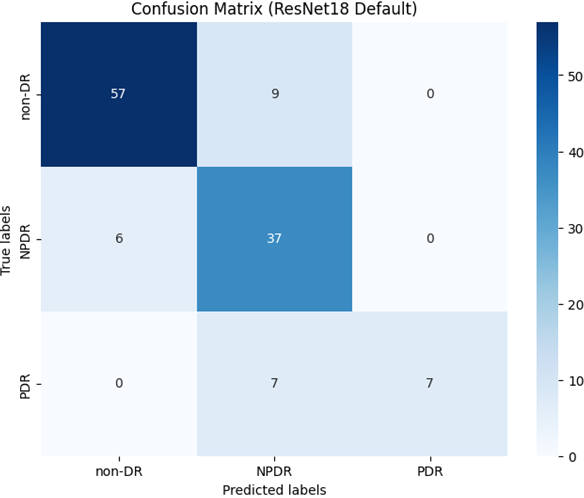
\includegraphics[width=7cm]{gambar/confusionMatrixResnet18_bestVal.png} }}%
	\qquad
	\subfloat[\centering Last Trained ResNet-18]{{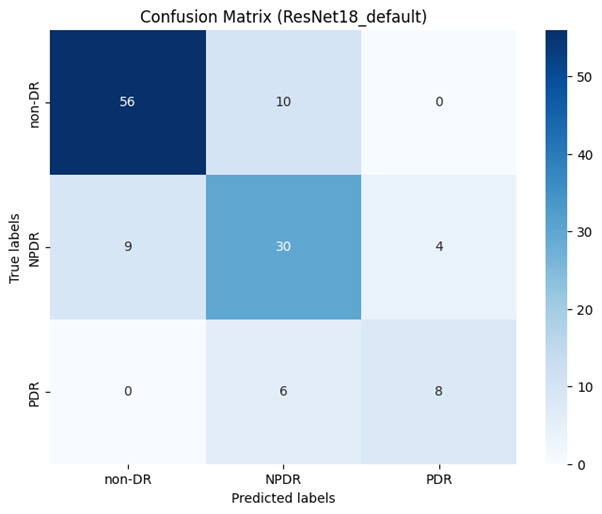
\includegraphics[width=7cm]{gambar/last model/confusionMatrixResnet18.png} }}%
	\caption{Confusion Matrix ResNet-18 yang Tidak Dilakukan Penyesuaian Beban Kelas}
	\label{fig:confRes18}
\end{figure}

\begin{itemize}
	\item Untuk dataset non-DR dapat dilihat bahwa model dapat melakukan prediksi \textbf{57 kasus non-DR} dengan akurat, dan 9 kasus diprediksi salah sebagai NDPR tanpa prediksi untuk PDR.
	
	\item Untuk dataset NPDR dapat dilihat bahwa model dapat melakukan prediksi \textbf{37 kasus NPDR} dengan akurat, dan 6 kasus diprediksi sebagai non-DR tanpa prediksi untuk PDR.
	
	\item Untuk dataset PDR dapat dilihat bahwa model dapat melakukan prediksi \textbf{8 kasus PDR} dengan akurat, dan 6 kasus diprediksi sebagai NPDR tanpa prediksi non-DR.
\end{itemize}
\pagebreak

\begin{figure}[hbtp]
	\centering
	\subfloat[\centering Best Train acc ResNet-34]{{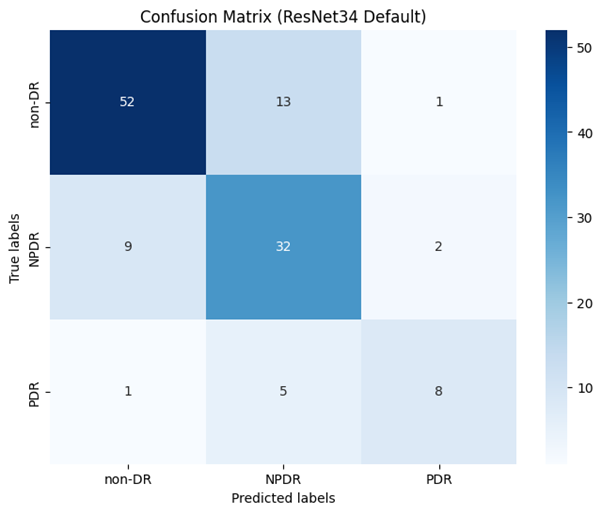
\includegraphics[width=7cm]{gambar/confusionMatrixResnet34_bestTrain.png} }}%
	\qquad
	\subfloat[\centering Best Val acc ResNet-34]{{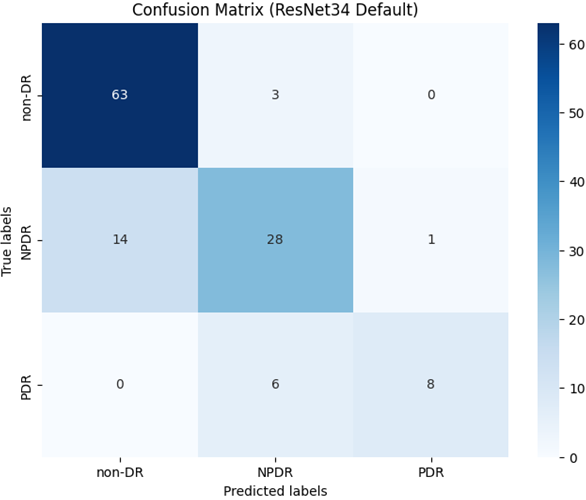
\includegraphics[width=7cm]{gambar/confusionMatrixResnet34_bestVal.png} }}%
	\qquad
	\subfloat[\centering Last Trained ResNet-34]{{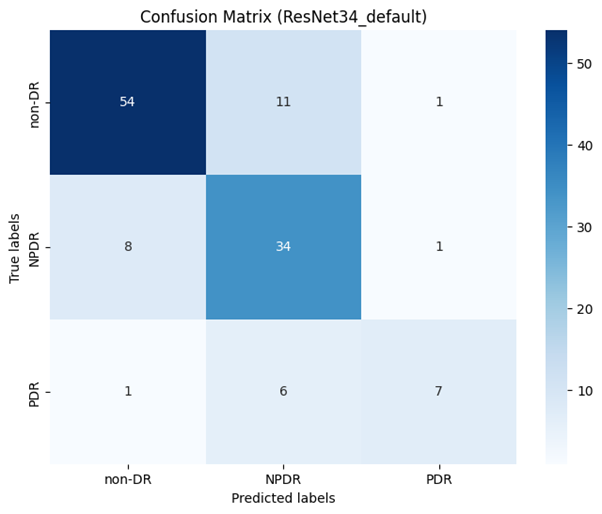
\includegraphics[width=7cm]{gambar/last model/confusionMatrixResnet34.png} }}%
	\caption{Confusion Matrix ResNet-34 yang Tidak Dilakukan Penyesuaian Beban Kelas}
	\label{fig:confRes34}
\end{figure}

\begin{itemize}
	\item Untuk dataset non-DR dapat dilihat bahwa model dapat melakukan prediksi \textbf{63 kasus non-DR} dengan akurat, dan 3 kasus diprediksi salah sebagai NDPR tanpa prediksi untuk PDR.
	
	\item Untuk dataset NPDR dapat dilihat bahwa model dapat melakukan prediksi \textbf{34 kasus NPDR} dengan akurat, 8 kasus diprediksi sebagai non-DR, dan 1 kasus diprediksi sebagai PDR.
	
	\item Untuk dataset PDR dapat dilihat bahwa model dapat melakukan prediksi \textbf{8 kasus PDR} dengan akurat, dan 6 kasus diprediksi sebagai NPDR tanpa prediksi non-DR.
\end{itemize}
\pagebreak

\begin{figure}[hbtp]
	\centering
	\subfloat[\centering Best Train acc ResNet-50]{{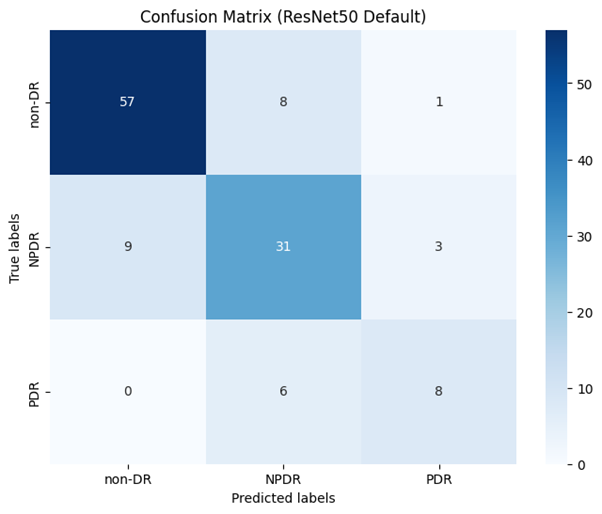
\includegraphics[width=7cm]{gambar/confusionMatrixResnet50_bestTrain.png} }}%
	\qquad
	\subfloat[\centering Best Val acc ResNet-50]{{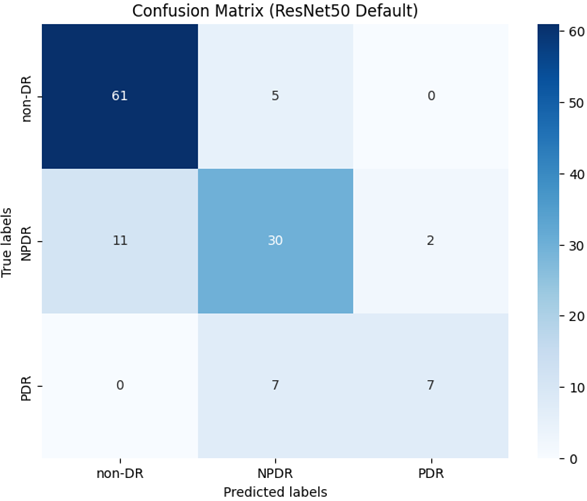
\includegraphics[width=7cm]{gambar/confusionMatrixResnet50_bestVal.png} }}%
	\qquad
	\subfloat[\centering Last Trained ResNet-50]{{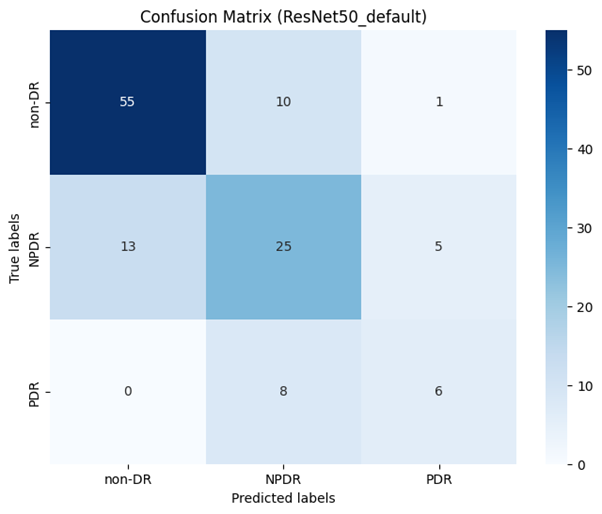
\includegraphics[width=7cm]{gambar/last model/confusionMatrixResnet50.png} }}%
	\caption{Confusion Matrix ResNet-50 Default yang Tidak Dilakukan Penyesuaian Beban Kelas}
	\label{fig:confRes50}
\end{figure}

\begin{itemize}
	\item Untuk dataset non-DR dapat dilihat bahwa model dapat melakukan prediksi \textbf{61 kasus non-DR} dengan akurat, dan 5 kasus diprediksi salah sebagai NDPR tanpa prediksi untuk PDR.
	
	\item Untuk dataset NPDR dapat dilihat bahwa model dapat melakukan prediksi \textbf{31 kasus NPDR} dengan akurat, 9 kasus diprediksi sebagai non-DR, dan 3 kasus diprediksi sebagai PDR.
	
	\item Untuk dataset PDR dapat dilihat bahwa model dapat melakukan prediksi \textbf{8 kasus PDR} dengan akurat, dan 6 kasus diprediksi sebagai NPDR tanpa prediksi non-DR.
\end{itemize}
\pagebreak

\begin{figure}[hbtp]
	\centering
	\subfloat[\centering Best Train acc ResNet-101]{{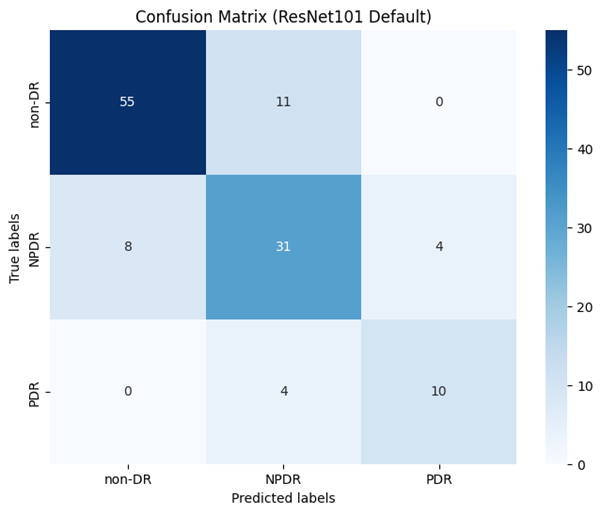
\includegraphics[width=7cm]{gambar/confusionMatrixResnet101_bestTrain.png} }}%
	\qquad
	\subfloat[\centering Best Val acc ResNet-101]{{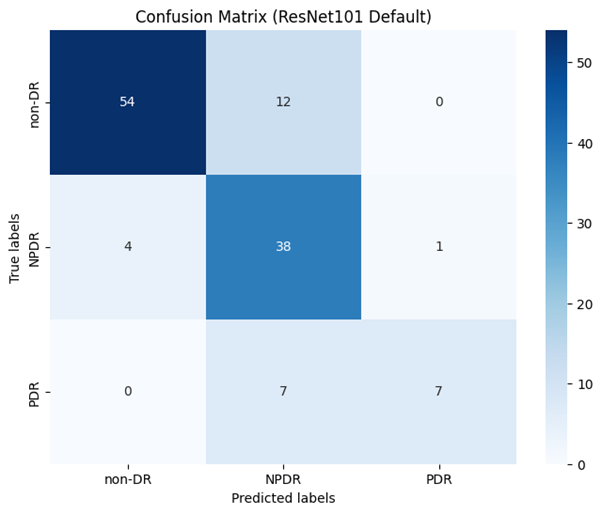
\includegraphics[width=7cm]{gambar/confusionMatrixResnet101_bestVal.png} }}%
	\qquad
	\subfloat[\centering Last Trained ResNet-101]{{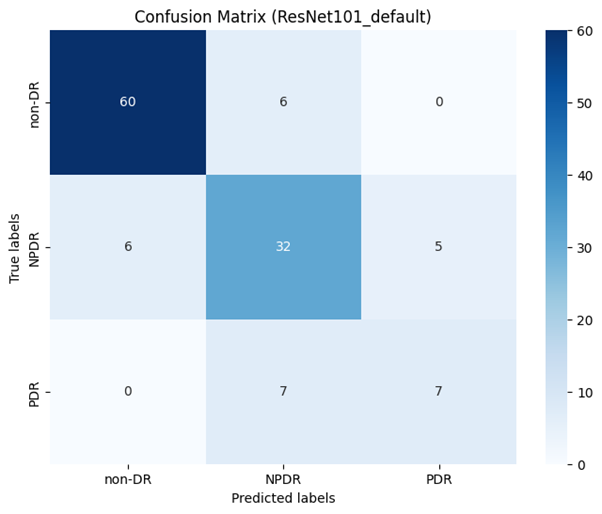
\includegraphics[width=7cm]{gambar/last model/confusionMatrixResnet101.png} }}%
	\caption{Confusion Matrix ResNet-101 yang Tidak Dilakukan Penyesuaian Beban Kelas}
	\label{fig:confRes101}
\end{figure}

\begin{itemize}
	\item Untuk dataset non-DR dapat dilihat bahwa model dapat melakukan prediksi \textbf{60 kasus non-DR} dengan akurat, dan 6 kasus diprediksi salah sebagai NDPR tanpa prediksi untuk PDR.
	
	\item Untuk dataset NPDR dapat dilihat bahwa model dapat melakukan prediksi \textbf{38 kasus NPDR} dengan akurat, 4 kasus diprediksi sebagai non-DR, dan 1 kasus diprediksi sebagai PDR.
	
	\item Untuk dataset PDR dapat dilihat bahwa model dapat melakukan prediksi \textbf{10 kasus PDR} dengan akurat, dan 4 kasus diprediksi sebagai NPDR tanpa prediksi non-DR.
\end{itemize}
\pagebreak

\begin{figure}[hbtp]
	\centering
	\subfloat[\centering Best Train acc ResNet-152]{{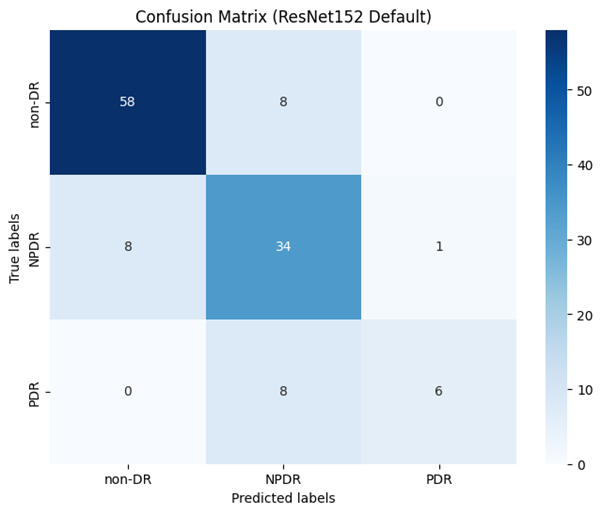
\includegraphics[width=7cm]{gambar/confusionMatrixResnet152_bestTrain.png} }}%
	\qquad
	\subfloat[\centering Best Val acc ResNet-152]{{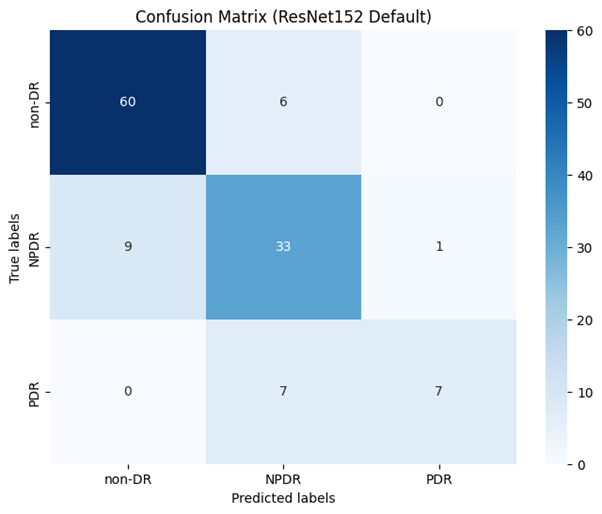
\includegraphics[width=7cm]{gambar/confusionMatrixResnet152_bestVal.png} }}%
	\qquad
	\subfloat[\centering Last Trained ResNet-152]{{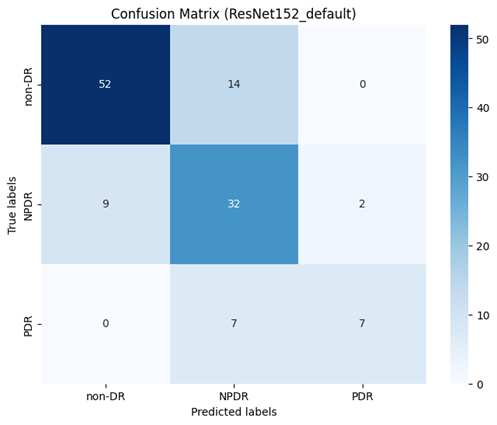
\includegraphics[width=7cm]{gambar/last model/confusionMatrixResnet152.png} }}%
	\caption{Confusion Matrix ResNet-152 yang Tidak Dilakukan Penyesuaian Beban Kelas}
	\label{fig:confRes152}
\end{figure}
\FloatBarrier

\begin{itemize}
	\item Untuk dataset non-DR dapat dilihat bahwa model terbaik adalah model best \emph{validation accuracy}, yang dapat melakukan prediksi \textbf{60 kasus non-DR} dengan akurat, dan 6 kasus diprediksi salah sebagai NDPR tanpa kasus diprediksi sebagai PDR.
	
	\item Untuk dataset NPDR dapat dilihat bahwa model terbaik adalah model \emph{best train accuracy}, yang dapat melakukan prediksi \textbf{34 kasus NPDR} dengan akurat, 8 kasus diprediksi sebagai non-DR, dan 1 kasus diprediksi sebagai PDR.
	
	\item Untuk dataset PDR dapat dilihat bahwa model terbaik adalah model \emph{best validation accuracy} dapat melakukan prediksi \textbf{7 kasus PDR} dengan akurat, 7 kasus diprediksi sebagai NPDR tanpa kasus diprediksi sebagai non-DR.
\end{itemize}
\pagebreak

\subsection{Hasil Pengujian Model dengan Menggunakan Penyesuaian \emph{Class-weight}}
\label{sec:412}
Proses testing untuk mendapatkan nilai QWK dilakukan dengan menggunakan data yang tidak dipergunakan saat training sebelumnya. Namun karena dataset testing tidak memiliki label, untuk metrik \emph{precision, recall}, dan \emph{F1-score} digunakan dataset validasi, yang sebesar 10\% dari dataset training. Model yang digunakan adalah model dengan metrik validasi terbaik, training terbaik, dan model terakhir dari setiap arsitektur.  Hasil pengujian metrik yang telah disebutkan dapat dilihat pada tabel \ref{tb:HasilTrainClassWeight}, tabel \ref{tb:HasilValClassWeight}, dan tabel \ref{tb:HasilLastClassWeight}
\begin{table}[hbtp]
	\begin{center}
		\caption{Hasil best trained model menggunakan Penyesuaian Beban Class}
		\label{tb:HasilTrainClassWeight}
		\begin{tabular}{|c|l|c|l|l|l|c|}
			\hline
			\rowcolor[HTML]{C0C0C0} 
			Arsitektur & \multicolumn{1}{c|}{\cellcolor[HTML]{C0C0C0}class} & acc                      & \multicolumn{1}{c|}{\cellcolor[HTML]{C0C0C0}prec} & \multicolumn{1}{c|}{\cellcolor[HTML]{C0C0C0}rec} & \multicolumn{1}{c|}{\cellcolor[HTML]{C0C0C0}F1} & QWK                                  \\ \hline
			& non-DR                                             &                          & 0,875                                             & \textbf{0,848485}                                & 0,861538                                        &                                      \\ \cline{2-2} \cline{4-6}
			& NPDR                                               &                          & 0,704545                                          & \textbf{0,72093}                                 & \textbf{0,712644}                               &                                      \\ \cline{2-2} \cline{4-6}
			\multirow{-3}{*}{ResNet-18}  & PDR                                                & \multirow{-3}{*}{\textbf{0,7886}} & \textbf{0,666667}                        & 0,714286                                         & 0,689655                                        & \multirow{-3}{*}{\textbf{0.7526956474324895}} \\ \hline
			& non-DR                                             &                          & 0,877193                                          & 0,757576                                         & 0,813008                                        &                                      \\ \cline{2-2} \cline{4-6}
			& NPDR                                               &                          & 0,617021                                          & 0,674419                                         & 0,644444                                        &                                      \\ \cline{2-2} \cline{4-6}
			\multirow{-3}{*}{ResNet-34}  & PDR                                                & \multirow{-3}{*}{0,7236} & 0,526316                                          & 0,714286                                         & 0,606061                                        & \multirow{-3}{*}{0.7344195070936137} \\ \hline
			& non-DR                                             &                          & 0,848485                                          & \textbf{0,848485}                                & 0,848485                                        &                                      \\ \cline{2-2} \cline{4-6}
			& NPDR                                               &                          & 0,634146                                          & 0,604651                                         & 0,619048                                        &                                      \\ \cline{2-2} \cline{4-6}
			\multirow{-3}{*}{ResNet-50}  & PDR                                                & \multirow{-3}{*}{0,7317} & 0,5                                               & 0,571429                                         & 0,533333                                        & \multirow{-3}{*}{0.7416221605070141} \\ \hline
			& non-DR                                             &                          & \textbf{0,916667}                                 & 0,833333                                         & \textbf{0,873016}                               &                                      \\ \cline{2-2} \cline{4-6}
			& NPDR                                               &                          & 0,666667                                          & 0,651163                                         & 0,658824                                        &                                      \\ \cline{2-2} \cline{4-6}
			\multirow{-3}{*}{ResNet-101} & PDR                                                & \multirow{-3}{*}{0,7642} & 0,52381                                           & 0,785714                                         & 0,628571                                        & \multirow{-3}{*}{0.7133252550521831} \\ \hline
			& non-DR                                             &                          & 0,870968                                          & 0,818182                                         & 0,84375                                         &                                      \\ \cline{2-2} \cline{4-6}
			& NPDR                                               &                          & \textbf{0,714286}                                 & 0,697674                                         & 0,705882                                        &                                      \\ \cline{2-2} \cline{4-6}
			\multirow{-3}{*}{ResNet-152} & PDR                                                & \multirow{-3}{*}{0,7805} & 0,631579                                          & \textbf{0,857143}                                & \textbf{0,727273}                               & \multirow{-3}{*}{0.7423939072743689} \\ \hline
		\end{tabular}
	\end{center}
\end{table}

Dari model terakhir yang telah dilatih, didapatkan nilai akurasi terbaik sebesar \textbf{0,7886} dari arsitektur \emph{ResNet-18}.

\begin{itemize}
	
	\item Untuk dataset non-DR didapatkan nilai precision sebesar \textbf{0,916667} dari arsitektur \emph{ResNet-101}, recall \textbf{0,848485} yang didapatkan pada arsitektur \emph{Resnet-18} dan \emph{ResNet-50}, dan F1 sebesar \textbf{0,873016} dari arsitektur \emph{ResNet-101};
	
	\item Untuk dataset NPDR didapatkan nilai precision sebesar \textbf{0,714286} dari arsitektur \emph{ResNet-152}, nilai recall sebesar \textbf{0,72093} dari arsitektur \emph{ResNet-18}, nilai F1 sebesar \textbf{0,712644} dari arsitektur \emph{ResNet-18};
	
	\item Untuk dataset PDR didapatkan nilai precision sebesar \textbf{0,667} dari arsitektur \emph{ResNet-18}, nilai recall sebesar \textbf{0,857143} dari arsitektur \emph{ResNet-152}, nilai F1 sebesar \textbf{0,727273} dari arsitektur \emph{ResNet-152}.
	
\end{itemize}

Dari seluruh arsitektur \emph{ResNet} yang digunakan, nilai QWK tertinggi sebesar \textbf{0.7526956474324895} didapatkan dari arsitektur \emph{ResNet-18}. Untuk hasil dari best validated model dari setiap arsitektur ResNet dapat dilihat pada tabel \ref{tb:HasilValClassWeight}

\pagebreak

\begin{table}[H]
	\begin{center}
		\caption{Hasil best validated model menggunakan Penyesuaian Beban Class}
		\label{tb:HasilValClassWeight}
		\begin{tabular}{|c|l|c|l|l|l|c|}
			\hline
			\rowcolor[HTML]{C0C0C0} 
			Arsitektur & \multicolumn{1}{c|}{\cellcolor[HTML]{C0C0C0}class} & acc                      & prec     & rec      & F1       & QWK                                  \\ \hline
			& non-DR                                             &                          & 0,869565 & 0,909091 & 0,888889 &                                      \\ \cline{2-2} \cline{4-6}
			& NPDR                                               &                          & 0,717391 & \textbf{0,767442} & 0,741573 &                             \\ \cline{2-2} \cline{4-6}
			\multirow{-3}{*}{ResNet-18}  & PDR                                                & \multirow{-3}{*}{\textbf{0,813}}  & \textbf{0,875}    & 0,5      & 0,636364 & \multirow{-3}{*}{0.6266311390141076} \\ \hline
			& non-DR                                             &                          & 0,777778 & \textbf{0,954545} & 0,857143 &                             \\ \cline{2-2} \cline{4-6}
			& NPDR                                               &                          & \textbf{0,88}     & 0,511628 & 0,647059 &                              \\ \cline{2-2} \cline{4-6}
			\multirow{-3}{*}{ResNet-34}  & PDR                                                & \multirow{-3}{*}{0,7886} & 0,705882 & \textbf{0,857143} & 0,774194 & \multirow{-3}{*}{0.6915275416648504} \\ \hline
			& non-DR                                             &                          & 0,84058  & 0,878788 & 0,859259 &                                      \\ \cline{2-2} \cline{4-6}
			& NPDR                                               &                          & 0,690476 & 0,674419 & 0,682353 &                                      \\ \cline{2-2} \cline{4-6}
			\multirow{-3}{*}{ResNet-50}  & PDR                                                & \multirow{-3}{*}{0,7805} & 0,75     & 0,642857 & 0,692308 & \multirow{-3}{*}{\textbf{0.7084479219119185}} \\ \hline
			& non-DR                                             &                          & \textbf{0,907692} & 0,893939 & \textbf{0,900763} &                    \\ \cline{2-2} \cline{4-6}
			& NPDR                                               &                          & 0,72973  & 0,627907 & 0,675    &                                      \\ \cline{2-2} \cline{4-6}
			\multirow{-3}{*}{ResNet-101} & PDR                                                & \multirow{-3}{*}{0,7886} & 0,52381  & 0,785714 & 0,628571 & \multirow{-3}{*}{0.7076588090504592} \\ \hline
			& non-DR                                             &                          & 0,870968 & 0,818182 & 0,84375  &                                      \\ \cline{2-2} \cline{4-6}
			& NPDR                                               &                          & 0,733333 & \textbf{0,767442} & \textbf{0,75}     &                    \\ \cline{2-2} \cline{4-6}
			\multirow{-3}{*}{ResNet-152} & PDR                                                & \multirow{-3}{*}{0,8049} & 0,75     & \textbf{0,857143} & \textbf{0,8}      & \multirow{-3}{*}{0.7052973650209466} \\ \hline
		\end{tabular}
	\end{center}
\end{table}

Dari model terakhir yang telah dilatih, didapatkan nilai akurasi terbaik sebesar \textbf{0,813} dari arsitektur \emph{ResNet-18}.

\begin{itemize}
	
	\item Untuk dataset non-DR didapatkan nilai precision sebesar \textbf{0,907692} dari arsitektur \emph{ResNet-101}, recall \textbf{0,954545} dari arsitektur \emph{ResNet-34}, dan F1 sebesar \textbf{0,900763} dari arsitektur \emph{ResNet-101};
	
	\item Untuk dataset NPDR didapatkan nilai precision sebesar \textbf{0,88} dari arsitektur \emph{ResNet-34}, nilai recall sebesar \textbf{0,767442} dari arsitektur \emph{ResNet-18} dan \textbf{0,767442}, nilai F1 sebesar \textbf{0,75} dari arsitektur \emph{ResNet-152};
	
	\item Untuk dataset PDR didapatkan nilai precision sebesar \textbf{0,875} dari arsitektur \emph{ResNet-18}, nilai recall sebesar \textbf{0,857143} dari arsitektur \emph{ResNet-34} dan arsitektur \emph{ResNet-152}, nilai F1 sebesar \textbf{0,8} dari arsitektur \emph{ResNet-152}.
	
\end{itemize}

Dari seluruh arsitektur \emph{ResNet} yang digunakan, nilai QWK tertinggi sebesar \textbf{0.7084479219119185} didapatkan dari arsitektur \emph{ResNet-50}. Untuk hasil dari model epoch terakhir dari setiap arsitektur ResNet dapat dilihat pada tabel \ref{tb:HasilLastClassWeight}

\pagebreak

\begin{table}[hbtp]
	\begin{center}
		\caption{Hasil Last Trained Model Menggunakan Penyesuaian Beban Class}
		\label{tb:HasilLastClassWeight}
		\begin{tabular}{|c|l|c|l|l|l|c|}
			\hline
			\rowcolor[HTML]{C0C0C0} 
			Arsitektur & \multicolumn{1}{c|}{\cellcolor[HTML]{C0C0C0}class} & acc                      & \multicolumn{1}{c|}{\cellcolor[HTML]{C0C0C0}prec} & \multicolumn{1}{c|}{\cellcolor[HTML]{C0C0C0}rec} & \multicolumn{1}{c|}{\cellcolor[HTML]{C0C0C0}F1} & QWK                                  \\ \hline
			& non-DR                                             &                          & 0,852941                                          & 0,878788                                         & 0,865672                                        &                                      \\ \cline{2-2} \cline{4-6}
			& NPDR                                               &                          & 0,710526                                          & 0,627907                                         & 0,666667                                        &                                      \\ \cline{2-2} \cline{4-6}
			\multirow{-3}{*}{ResNet-18}  & PDR                                                & \multirow{-3}{*}{\textbf{0,7724}} & 0,588235                                 & 0,714286                                         & 0,645161                                        & \multirow{-3}{*}{0.714979444673576}  \\ \hline
			& non-DR                                             &                          & 0,857143                                          & 0,818182                                         & 0,837209                                        &                                      \\ \cline{2-2} \cline{4-6}
			& NPDR                                               &                          & 0,652174                                          & 0,697674                                         & 0,674157                                        &                                      \\ \cline{2-2} \cline{4-6}
			\multirow{-3}{*}{ResNet-34}  & PDR                                                & \multirow{-3}{*}{0,748}  & 0,571429                                          & 0,571429                                         & 0,571429                                        & \multirow{-3}{*}{0.7137225555570403} \\ \hline
			& non-DR                                             &                          & 0,822581                                          & 0,772727                                         & 0,796875                                        &                                      \\ \cline{2-2} \cline{4-6}
			& NPDR                                               &                          & 0,608696                                          & 0,651163                                         & 0,629213                                        &                                      \\ \cline{2-2} \cline{4-6}
			\multirow{-3}{*}{ResNet-50}  & PDR                                                & \multirow{-3}{*}{0,7236} & 0,666667                                          & 0,714286                                         & 0,689655                                        & \multirow{-3}{*}{0.7006591702210159} \\ \hline
			& non-DR                                             &                          & 0,901639                                          & 0,833333                                         & 0,866142                                        &                                      \\ \cline{2-2} \cline{4-6}
			& NPDR                                               &                          & 0,666667                                          & 0,697674                                         & 0,681818                                        &                                      \\ \cline{2-2} \cline{4-6}
			\multirow{-3}{*}{ResNet-101} & PDR                                                & \multirow{-3}{*}{\textbf{0,7724}} & 0,588235                                 & 0,714286                                         & 0,645161                                        & \multirow{-3}{*}{\textbf{0.7422994855414904}} \\ \hline
			& non-DR                                             &                          & 0,892857                                          & 0,757576                                         & 0,819672                                        &                                      \\ \cline{2-2} \cline{4-6}
			& NPDR                                               &                          & 0,604167                                          & 0,674419                                         & 0,637363                                        &                                      \\ \cline{2-2} \cline{4-6}
			\multirow{-3}{*}{ResNet-152} & PDR                                                & \multirow{-3}{*}{0,7154} & 0,473684                                          & 0,642857                                         & 0,545455                                        & \multirow{-3}{*}{0.727319861566579}  \\ \hline
		\end{tabular}
	\end{center}
\end{table}

Dari model terakhir yang telah dilatih, didapatkan nilai akurasi terbaik sebesar \textbf{0,7724} dari arsitektur \emph{ResNet-18} dan \emph{ResNet-101}.

\begin{itemize}
	
	\item Untuk dataset non-DR didapatkan nilai precision sebesar \textbf{0,907692} dari arsitektur \emph{ResNet-101}, recall \textbf{0,954545} dari arsitektur \emph{ResNet-34}, dan F1 sebesar \textbf{0,900763} dari arsitektur \emph{ResNet-101};
	
	\item Untuk dataset NPDR didapatkan nilai precision sebesar \textbf{0,88} dari arsitektur \emph{ResNet-34}, nilai recall sebesar \textbf{0,767442} dari arsitektur \emph{ResNet-18} dan \textbf{0,767442}, nilai F1 sebesar \textbf{0,75} dari arsitektur \emph{ResNet-152};
	
	\item Untuk dataset PDR didapatkan nilai precision sebesar \textbf{0,875} dari arsitektur \emph{ResNet-18}, nilai recall sebesar \textbf{0,857143} dari arsitektur \emph{ResNet-34} dan arsitektur \emph{ResNet-152}, nilai F1 sebesar \textbf{0,8} dari arsitektur \emph{ResNet-152}.
	
\end{itemize}

Dari seluruh arsitektur \emph{ResNet} yang digunakan, nilai QWK tertinggi sebesar \textbf{0.7422994855414904} didapatkan dari arsitektur \emph{ResNet-101}.

Grafik dari \emph{training loss}, \emph{training accuracy}, dan \emph{validation accuracy} pada setiap arsitektur tanpa menggunakan penyesuaian \emph{class weight} dapat dilihat dengan lebih jelas pada Gambar \ref{Fig:GraphTrainingDefPt2} Nilai loss cukup tinggi pada permulaan dikarenakan ukuran \emph{batch} yang cukup kecil, sehingga jumlah training sample yang digunakan dalam satu batch untuk satu iterasi juga kecil. Namun, setelah epoch tertentu, model akan menjaga nilai loss-nya tetap stabil pada nilai yang relatif rendah.
\pagebreak

\begin{figure}[hbtp]
	\centering
	\subfloat[\centering Training Loss dan akurasi ResNet-18]{{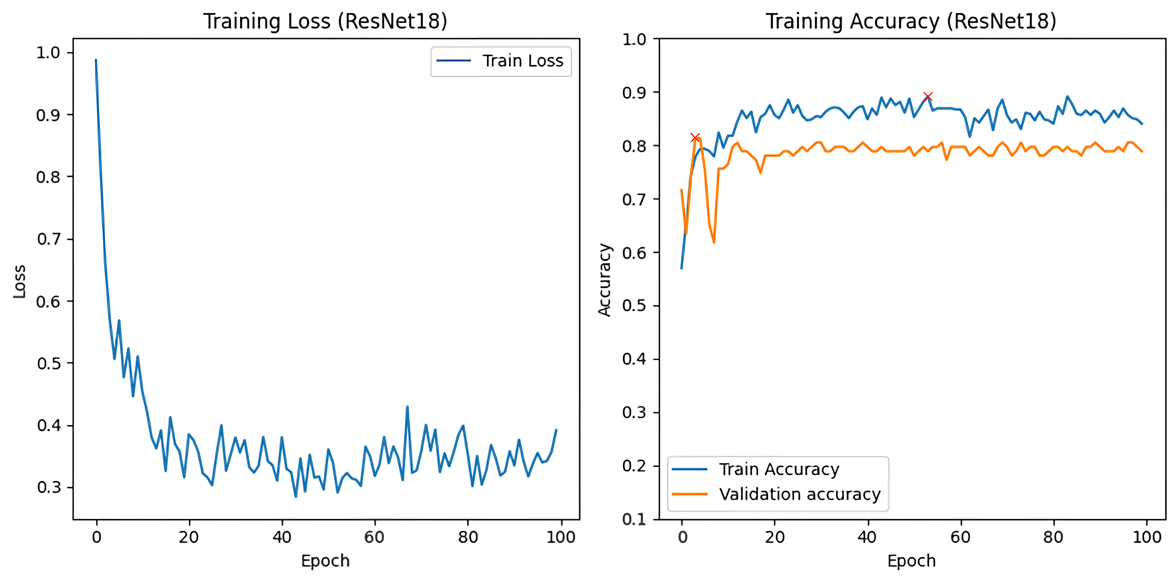
\includegraphics[height=7cm]{gambar/TrainingGraphResNet18class-weighted.png}}}
	\qquad
	\subfloat[\centering Training Loss dan akurasi ResNet-34]{{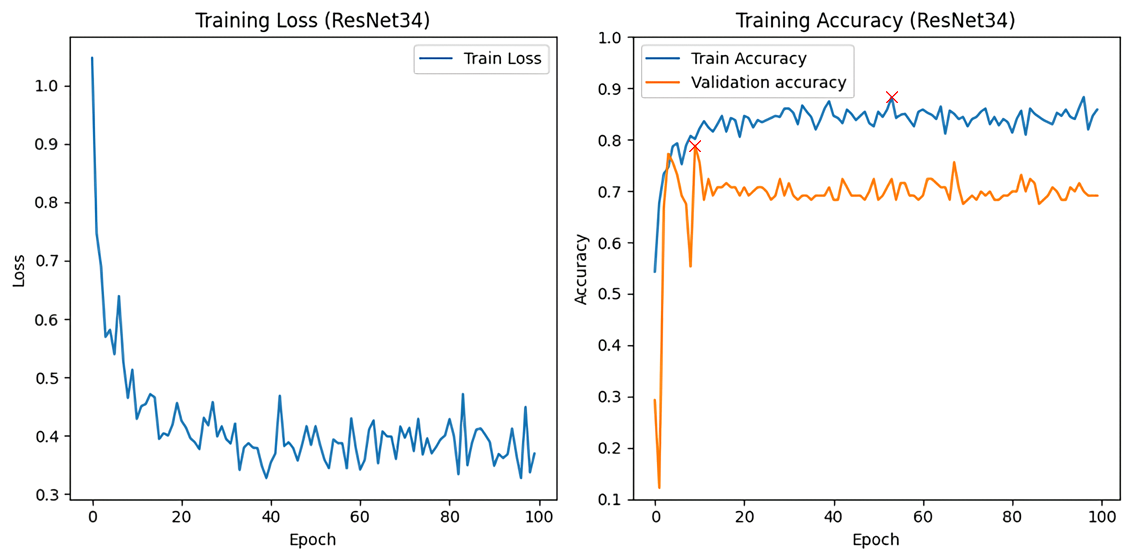
\includegraphics[height=7cm]{gambar/TrainingGraphResNet34class-weighted.png}}}
	\caption{Grafik Training Loss dan akurasi ResNet-18 dan ResNet-34 dengan Penyesuaian Beban pada \emph{Class}}
	\label{fig:graphTrainingWeightedPt1}
\end{figure}

Dari grafik Training Loss \emph{ResNet-18} dapat dilihat bahwa nilai loss mulai dari \textbf{1.0} dan dengan cepat menjadi stabil mendekati epoch ke-\textbf{20} dengan nilai menjadi fluktuatif di antara \textbf{0.3 dan 0.45}.

Dari grafik Training Accuracy \emph{ResNet-18} dapat dilihat bahwa akurasi training mulai dari nilai \textbf{0.6} dan dengan cepat menjadi stabil mendekati epoch ke-\textbf{10} dimana nilai berada di antara \textbf{0.8 dan 0.9} 

Dari grafik Training Accuracy \emph{ResNet-18} dapat dilihat bahwa akurasi validasi mulai dari nilai \textbf{0.7} dan bersifat fluktuatif hingga epoch ke-\textbf{20} dimana nilai menjadi stabil di antara \textbf{0.7 dan 0.8}.

Kemudian Dari grafik Training Loss \emph{ResNet-34} dapat dilihat bahwa nilai loss mulai dari \textbf{1.0} dan dengan cepat menjadi stabil mendekati epoch ke-\textbf{20} dengan nilai menjadi fluktuatif di antara \textbf{0.3 dan 0.5}.

Dari grafik Training Accuracy \emph{ResNet-34} dapat dilihat bahwa akurasi training mulai dari nilai \textbf{0.55} dan dengan cepat menjadi stabil mendekati epoch ke-\textbf{10} dimana nilai berada di antara \textbf{0.8 dan 0.9} 

Dari grafik Training Accuracy \emph{ResNet-34} dapat dilihat bahwa akurasi validasi mulai dari nilai \textbf{0.3}, kemudian turun mendekati nilai \textbf{0.1} sebelum kemudian naik kembali dan bersifat fluktuatif hingga epoch ke-\textbf{20} dimana nilai menjadi stabil di antara \textbf{0.7 dan 0.8}.

\begin{figure}[H]
	\centering
	\subfloat[\centering Training Loss dan akurasi ResNet-50]{{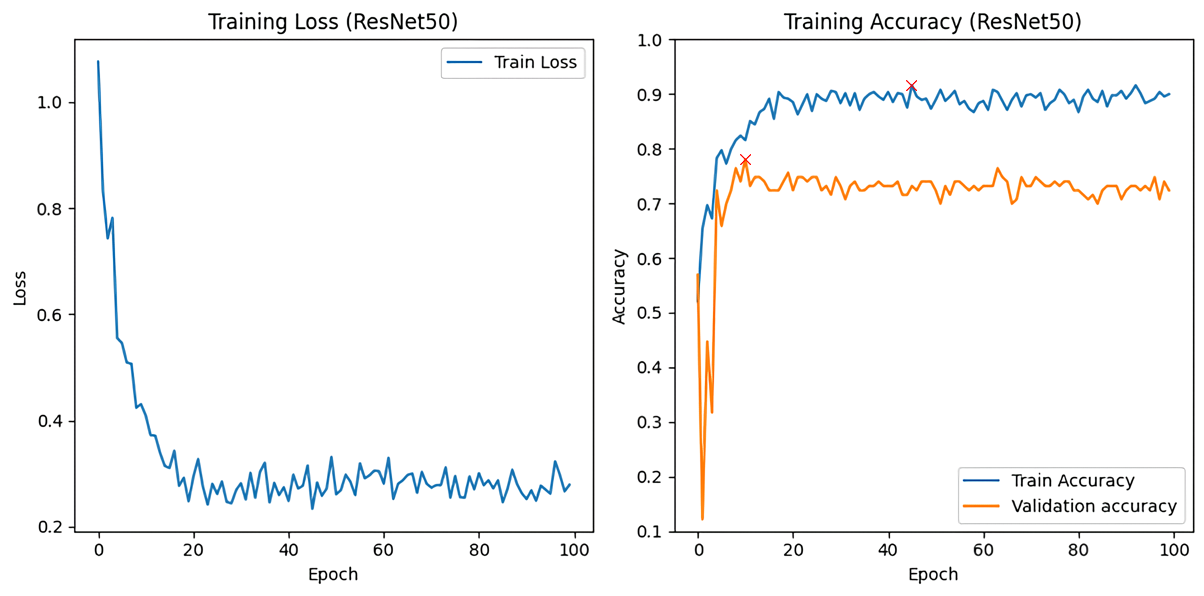
\includegraphics[height=7cm]{gambar/TrainingGraphResNet50class-weighted.png}}}
	\qquad
	\subfloat[\centering Training Loss dan akurasi ResNet-101]{{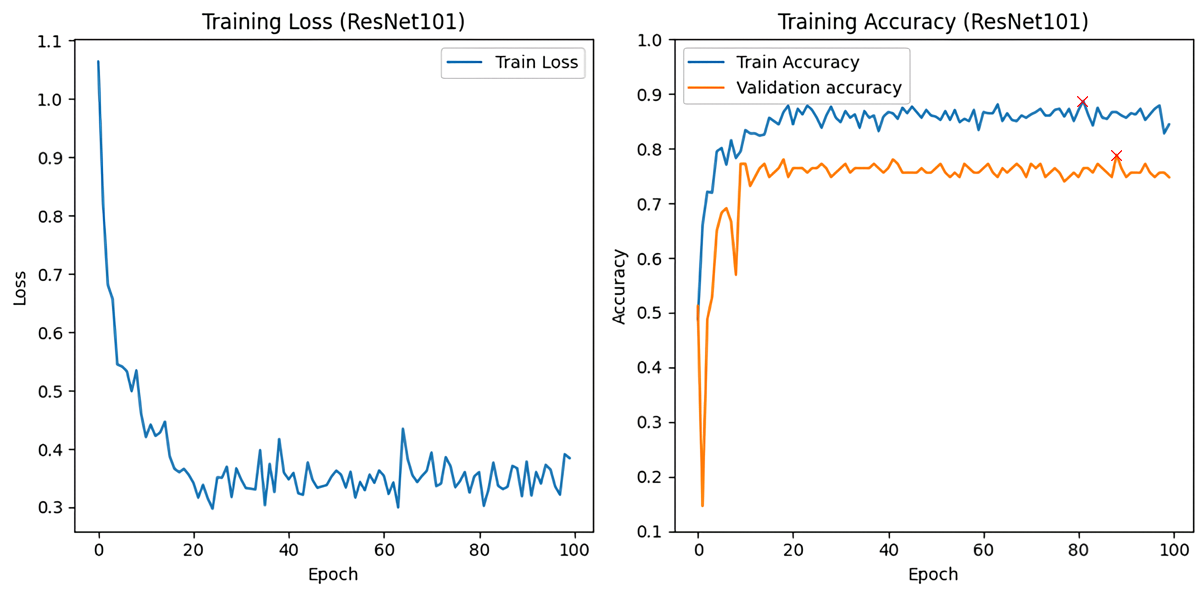
\includegraphics[height=7cm]{gambar/TrainingGraphResNet101class-weighted.png}}}
	\caption{Grafik Training Loss dan akurasi ResNet-50, 101 dengan Penyesuaian Beban pada \emph{Class}}
	\label{fig:graphTrainingWeightedPt2}
\end{figure}

Dari grafik Training Loss \emph{ResNet-50} dapat dilihat bahwa nilai loss mulai dari \textbf{1.05} dan dengan cepat menjadi stabil mendekati epoch ke-\textbf{20} dengan nilai menjadi fluktuatif di antara \textbf{0.3 dan 0.4}.

Dari grafik Training Accuracy \emph{ResNet-50} dapat dilihat bahwa akurasi training mulai dari nilai mendekati \textbf{0.6} dan dengan cepat menjadi stabil mendekati epoch ke-\textbf{10} dimana nilai berada di antara \textbf{0.8 dan 0.9} 

Dari grafik Training Accuracy \emph{ResNet-50} dapat dilihat bahwa akurasi validasi mulai dari nilai \textbf{0.6} kemudian turun mendekati \textbf{0.1} sebelum akhirnya naik kembali, dan bersifat fluktuatif hingga epoch ke-\textbf{10} dimana nilai menjadi stabil di antara \textbf{0.7 dan 0.8}.

Kemudian Dari grafik Training Loss \emph{ResNet-101} dapat dilihat bahwa nilai loss mulai dari mendekati \textbf{1.1} dan dengan cepat menjadi stabil mendekati epoch ke-\textbf{20} dengan nilai menjadi fluktuatif di antara \textbf{0.3 dan 0.45}.

Dari grafik Training Accuracy \emph{ResNet-101} dapat dilihat bahwa akurasi training mulai dari nilai \textbf{0.6} dan dengan cepat menjadi stabil mendekati epoch ke-\textbf{10} dimana nilai berada di antara \textbf{0.8 dan 0.9} 

Dari grafik Training Accuracy \emph{ResNet-101} dapat dilihat bahwa akurasi validasi mulai dari nilai \textbf{0.5} kemudian turun mendekati \textbf{0.1} sebelum akhirnya naik kembali dan bersifat fluktuatif hingga sebelum epoch ke-\textbf{20} dimana nilai menjadi stabil di antara \textbf{0.7 dan 0.8}.

\begin{figure}[H]
	\centering
	\subfloat[\centering Training Loss dan akurasi ResNet-152]{{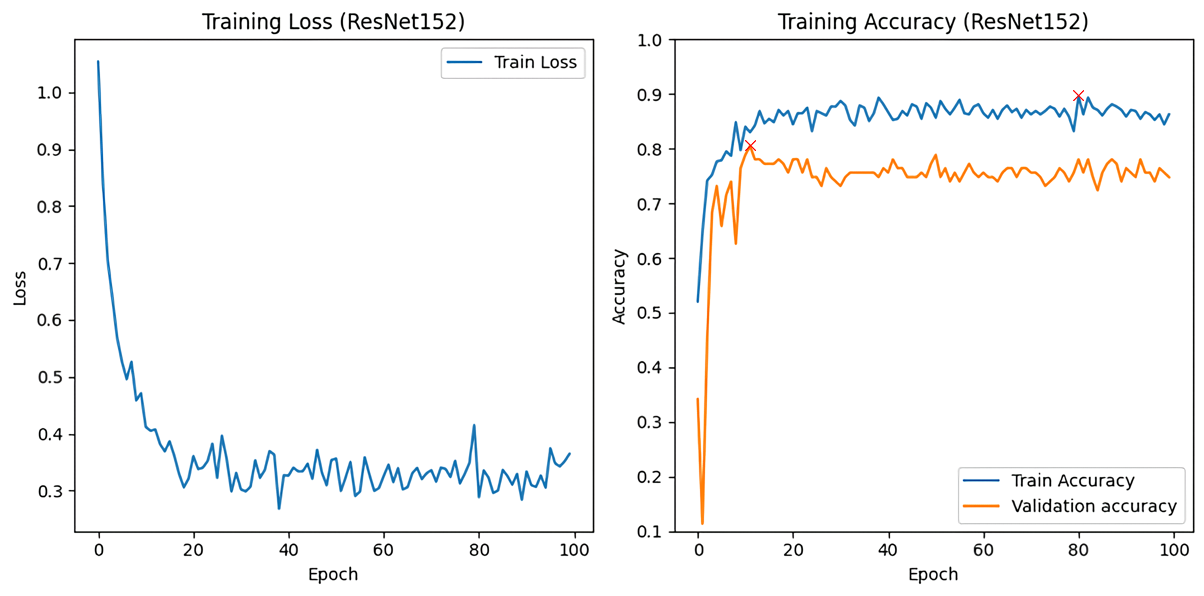
\includegraphics[height=7cm]{gambar/TrainingGraphResNet152class-weighted.png}}}
	\caption{Grafik Training Loss dan akurasi ResNet-152 dengan Penyesuaian Beban pada \emph{Class}}
	\label{fig:graphTrainingWeightedPt3}
\end{figure}

Dari grafik Training Loss \emph{ResNet-152} dapat dilihat bahwa nilai loss mulai dari \textbf{\>1.0} dan dengan cepat menjadi stabil mendekati epoch ke-\textbf{20} dengan nilai menjadi fluktuatif di antara \textbf{0.3 dan 0.45}.

Dari grafik Training Accuracy \emph{ResNet-152} dapat dilihat bahwa akurasi training mulai dari nilai \textbf{\>0.5} dan dengan cepat menjadi stabil mendekati epoch ke-\textbf{10} dimana nilai berada di antara \textbf{0.8 dan 0.9} 

Dari grafik Training Accuracy \emph{ResNet-152} dapat dilihat bahwa akurasi validasi mulai dari nilai antara \textbf{0.3} dan \textbf{0.4} kemudian turun mendekati \textbf{0.1} sebelum akhirnya naik dan bersifat fluktuatif hingga epoch ke-\textbf{20}. Dimana nilai menjadi stabil di antara \textbf{0.7 dan 0.8}.

Untuk \emph{confusion matrix} dari setiap arsitektur dapat dilihat pada Gambar \ref{fig:confRes18Class}, Gambar \ref{fig:confRes34Class}, Gambar \ref{fig:confRes50Class}, Gambar \ref{fig:confRes101Class}, dan Gambar \ref{fig:confRes152Class}. Masing - masing gambar terdiri dari tiga \emph{confusion matrix}, yang merupakan hasil dari model terbaik pada akurasi \emph{training}, model terbaik pada akurasi validasi, dan model terakhir dari 100 \emph{epoch} pada arsitektur tersebut.

\begin{figure}[hbtp]
	\centering
	\subfloat[\centering Best Train acc ResNet-18]{{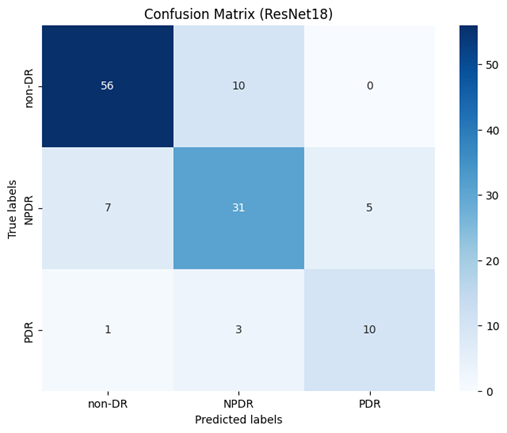
\includegraphics[width=7cm]{gambar/confusionMatrixResnet18class-weighted_bestTrain.png} }}%
	\qquad
	\subfloat[\centering Best Val acc ResNet-18]{{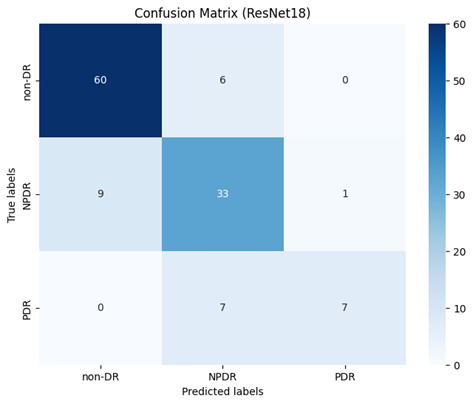
\includegraphics[width=7cm]{gambar/confusionMatrixResnet18class-weighted_bestVal.png} }}%
	\qquad
	\subfloat[\centering Last Trained ResNet-18]{{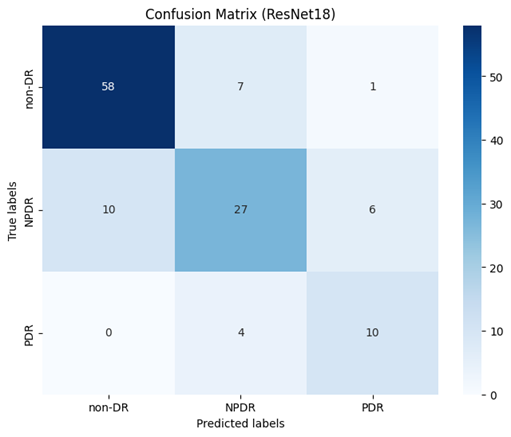
\includegraphics[width=7cm]{gambar/last model/confusionMatrixResnet18class-weighted.png} }}%
	\caption{Confusion Matrix ResNet-18 yang Telah dilakukan Penyesuaian Beban Kelas}
	\label{fig:confRes18Class}
\end{figure}

\begin{itemize}
	\item Untuk dataset non-DR dapat dilihat bahwa model terbaik adalah model \emph{best validation accuracy}, yang dapat melakukan prediksi \textbf{60 kasus non-DR} dengan akurat, dan 6 kasus diprediksi salah sebagai NDPR tanpa prediksi untuk PDR.
	
	\item Untuk dataset NPDR dapat dilihat bahwa model terbaik adalah model \emph{best validation accuracy}, yang dapat melakukan prediksi \textbf{33 kasus NPDR} dengan akurat, 9 kasus diprediksi sebagai non-DR, dan 1 kasus diprediksi sebagai PDR.
	
	\item Untuk dataset PDR dapat dilihat bahwa model terbaik dapat melakukan prediksi \textbf{10 kasus PDR} dengan akurat. Pada model \emph{best train}, 3 kasus diprediksi sebagai NPDR, dan 1 kasus diprediksi sebagai non-DR. Pada model \emph{last trained}, 4 kasus diprediksi sebagai NPDR tanpa prediksi non-DR.
\end{itemize}
\pagebreak

\begin{figure}
	\centering
	\subfloat[\centering Best Train acc ResNet-34]{{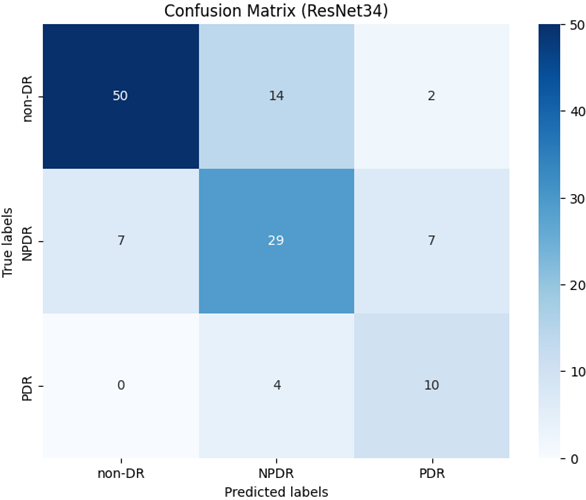
\includegraphics[width=7cm]{gambar/confusionMatrixResnet34class-weighted_bestTrain.png} }}%
	\qquad
	\subfloat[\centering Best Val acc ResNet-34]{{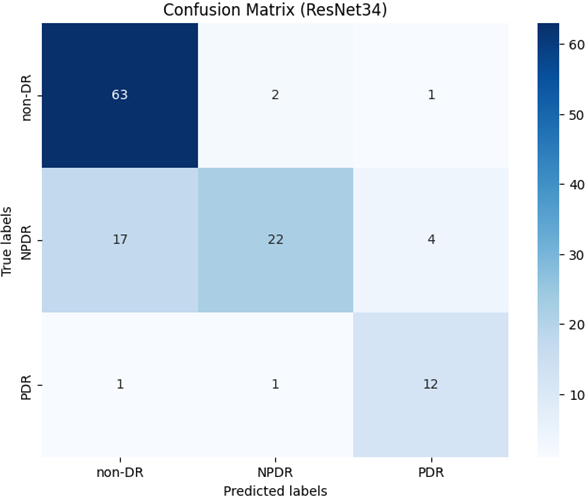
\includegraphics[width=7cm]{gambar/confusionMatrixResnet34class-weighted_bestVal.png} }}%
	\qquad
	\subfloat[\centering Last Trained ResNet-34]{{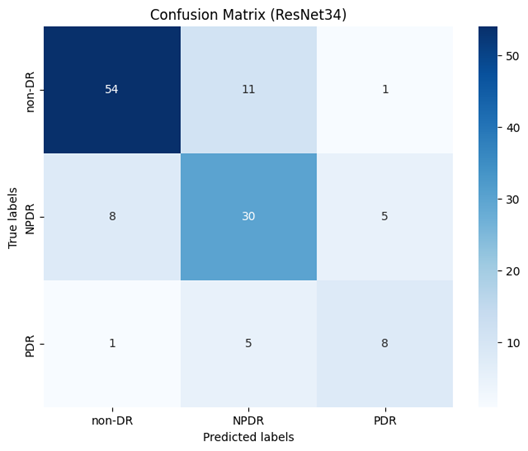
\includegraphics[width=7cm]{gambar/last model/confusionMatrixResnet34class-weighted.png} }}
	\caption{Confusion Matrix ResNet-34 yang Telah dilakukan Penyesuaian Beban Kelas}
	\label{fig:confRes34Class}
\end{figure}

\begin{itemize}
	\item Untuk dataset non-DR dapat dilihat bahwa model terbaik adalah model \emph{best validation accuracy}, yang dapat melakukan prediksi \textbf{63 kasus non-DR} dengan akurat, 2 kasus diprediksi salah sebagai NDPR, dan 1 kasus dirediksi sebagai PDR.
	\item Untuk dataset NPDR dapat dilihat bahwa model terbaik adalah model \emph{last trained}, yang dapat melakukan prediksi \textbf{30 kasus NPDR} dengan akurat, 8 kasus diprediksi sebagai non-DR, dan 5 kasus diprediksi sebagai PDR.
	\item Untuk dataset PDR dapat dilihat bahwa model terbaik adalah model \emph{best validation accuracy}, yang dapat melakukan prediksi \textbf{12 kasus PDR} dengan akurat, 1 kasus diprediksi sebagai NPDR, dan 1 kasus diprediksi sebagai non-DR.
\end{itemize}
\pagebreak

\begin{figure}[hbtp]
	\centering
	\subfloat[\centering Best Train acc ResNet-50]{{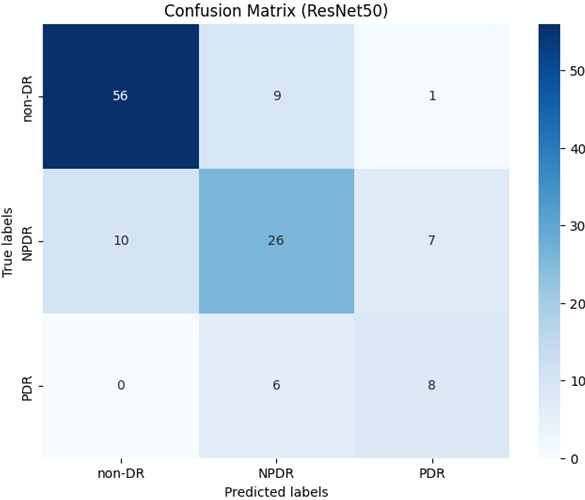
\includegraphics[width=7cm]{gambar/confusionMatrixResnet50class-weighted_bestTrain.png} }}%
	\qquad
	\subfloat[\centering Best Val acc ResNet-50]{{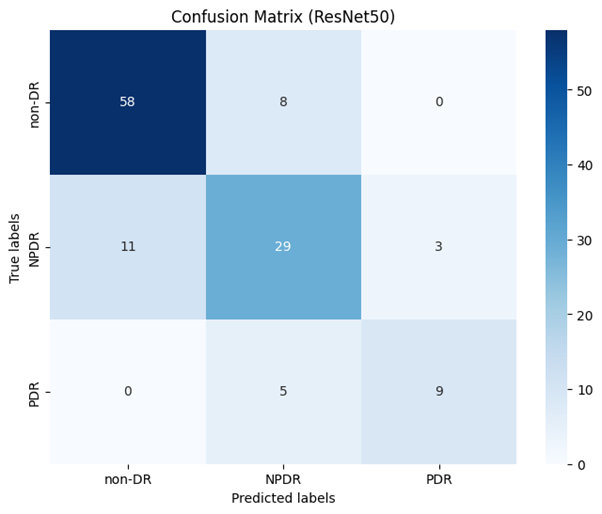
\includegraphics[width=7cm]{gambar/confusionMatrixResnet50class-weighted_bestVal.png} }}%
	\qquad
	\subfloat[\centering Last Trained ResNet-50]{{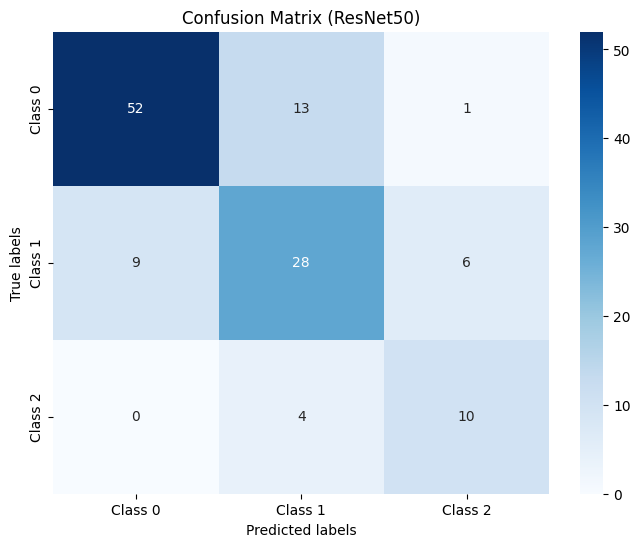
\includegraphics[width=7cm]{gambar/last model/confusionMatrixResnet50class-weighted.png} }}
	\caption{Confusion Matrix ResNet-50 yang Telah dilakukan Penyesuaian Beban Kelas}
	\label{fig:confRes50Class}
\end{figure}

\begin{itemize}
	\item Untuk dataset non-DR dapat dilihat bahwa model terbaik adalah model \emph{best validation accuracy}, yang dapat melakukan prediksi \textbf{58 kasus non-DR} dengan akurat, dan 8 kasus diprediksi salah sebagai NDPR tanpa prediksi untuk PDR.
	
	\item Untuk dataset NPDR dapat dilihat bahwa model terbaik adalah model \emph{best validation accuracy}, yang dapat melakukan prediksi \textbf{29 kasus NPDR} dengan akurat, 11 kasus diprediksi sebagai non-DR, dan 3 kasus diprediksi sebagai PDR.
	
	\item Untuk dataset PDR dapat dilihat bahwa model terbaik adalah model \emph{last trained}, yang dapat melakukan prediksi \textbf{10 kasus PDR} dengan akurat, dan 4 kasus diprediksi sebagai NPDR tanpa prediksi non-DR.
\end{itemize}
\pagebreak

\begin{figure}[hbtp]
	\centering
	\subfloat[\centering Best Train acc ResNet-101]{{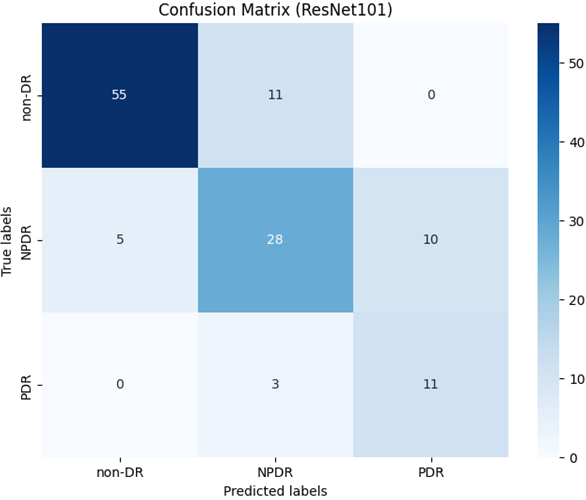
\includegraphics[width=7cm]{gambar/confusionMatrixResnet101class-weighted_bestTrain.png} }}%
	\qquad
	\subfloat[\centering Best Val acc ResNet-101]{{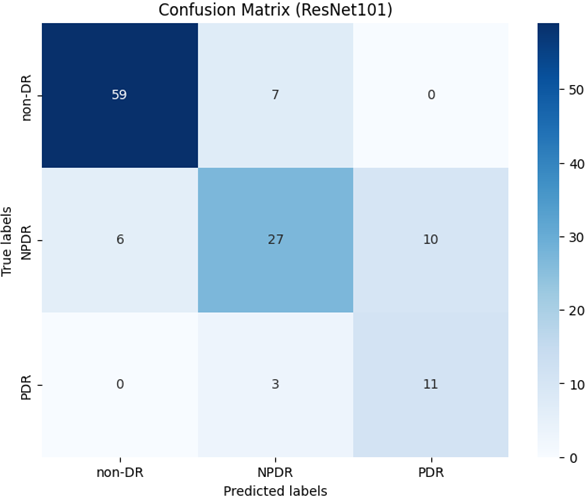
\includegraphics[width=7cm]{gambar/confusionMatrixResnet101class-weighted_bestVal.png} }}%
	\qquad
	\subfloat[\centering Last Trained ResNet-101]{{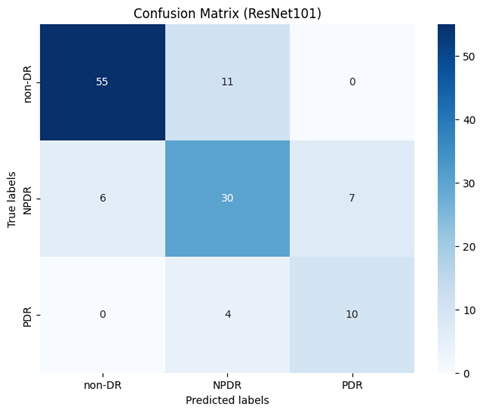
\includegraphics[width=7cm]{gambar/last model/confusionMatrixResnet101class-weighted.png} }}
	\caption{Confusion Matrix ResNet-101 yang Telah dilakukan Penyesuaian Beban Kelas}
	\label{fig:confRes101Class}
\end{figure}

\begin{itemize}
	\item Untuk dataset non-DR dapat dilihat bahwa model terbaik adalah model \emph{best validation accuracy}, yang dapat melakukan prediksi \textbf{59 kasus non-DR} dengan akurat, dan 7 kasus diprediksi salah sebagai NDPR. Tidak ada kasus yang diprediksi sebagai PDR.
	
	\item Untuk dataset NPDR dapat dilihat bahwa model terbaik adalah model \emph{last trained}, yang dapat melakukan prediksi \textbf{30 kasus NPDR} dengan akurat, 6 kasus diprediksi sebagai non-DR, dan 7 kasus diprediksi sebagai PDR.
	
	\item Untuk dataset PDR dapat dilihat bahwa model terbaik adalah model \emph{best train} dan \emph{best validation accuracy}, yang dapat melakukan prediksi \textbf{11 kasus PDR} dengan akurat, 3 kasus diprediksi sebagai NPDR. Tidak ada kasus yang diprediksi sebagai non-DR.
\end{itemize}
\pagebreak

\begin{figure}[hbtp]
	\centering
	\subfloat[\centering Best Train acc ResNet-152]{{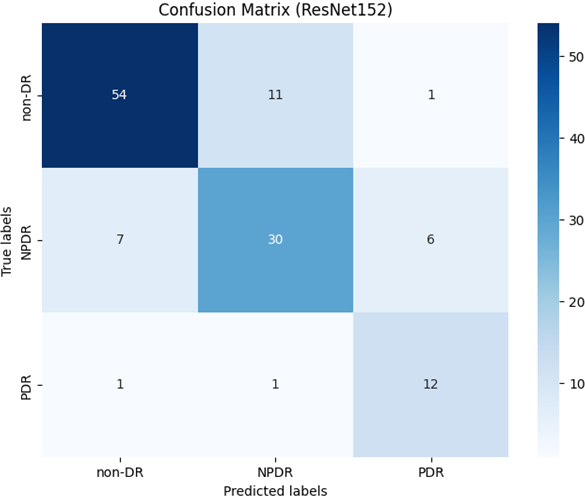
\includegraphics[width=7cm]{gambar/confusionMatrixResnet152class-weighted_bestTrain.png} }}%
	\qquad
	\subfloat[\centering Best Val acc ResNet-152]{{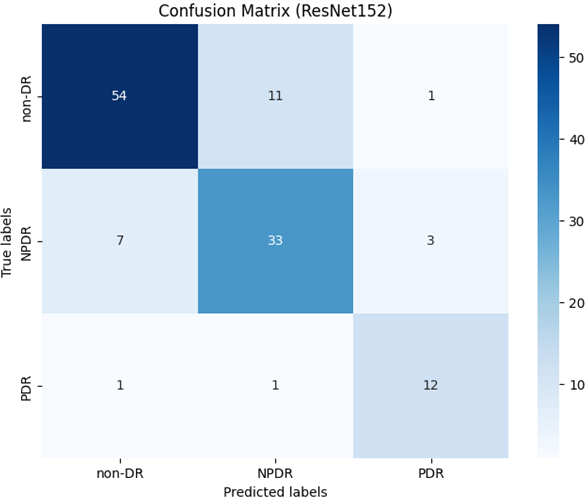
\includegraphics[width=7cm]{gambar/confusionMatrixResnet152class-weighted_bestVal.png} }}%
	\qquad
	\subfloat[\centering Last Trained ResNet-152]{{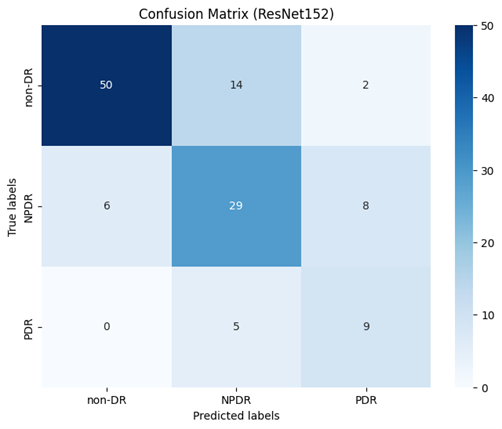
\includegraphics[width=7cm]{gambar/last model/confusionMatrixResnet152class-weighted.png} }}
	\caption{Confusion Matrix ResNet-152 yang Telah dilakukan Penyesuaian Beban Kelas}
	\label{fig:confRes152Class}
\end{figure}

\begin{itemize}
	\item Untuk dataset non-DR dapat dilihat bahwa model terbaik adalah model \emph{best train} dan \emph{best validation accuracy}, yang dapat melakukan prediksi \textbf{54 kasus non-DR} dengan akurat, dan 11 kasus diprediksi salah sebagai NDPR dan 1 kasus diprediksi sebagai PDR.
	
	\item Untuk dataset NPDR dapat dilihat bahwa model terbaik adalah model \emph{best validation accuracy}, yang dapat melakukan prediksi \textbf{33 kasus NPDR} dengan akurat, 7 kasus diprediksi sebagai non-DR, dan 3 kasus diprediksi sebagai PDR.
	
	\item Untuk dataset PDR dapat dilihat bahwa model terbaik adalah model \emph{best validation accuracy}, yang dapat melakukan prediksi \textbf{12 kasus PDR} dengan akurat, 1 kasus diprediksi sebagai NPDR, dan 1 kasus diprediksi sebagai non-DR.
\end{itemize}

\section{Analisis Hasil dan Evaluasi}
\label{sec:42}

Pengujian dilakukan dengan menggunakan model yang memiliki metrik akurasi tertinggi dalam setiap trainingnya. Terdapat dua skenario pengujian yang dilakukan dalam penelitian ini. Pertama, perbandingan untuk setiap arstitektur model yang digunakan tanpa dilakukan penyesuaian pada class-weight. Kedua, perbandingan untuk setiap arstitektur model yang digunakan dengan penerapan class-weight. Hasil perbandingan tersebut akan dilampirkan pada tabel dan nantinya akan dianalisa pada Tabel \ref{tb:PerbandinganHasilBestTrain}, Tabel \ref{tb:PerbandinganHasilBestVal}, dan Tabel \ref{tb:PerbandinganHasilLastTrained}.

\begin{table}[hbtp]
	\begin{center}
	\caption{Perbandingan Nilai Akurasi, Recall pada class PDR. dan QWK dari setiap \emph{Best Trained Model} dengan Pembebanan pada \emph{Class} dan tanpa Pembebanan pada \emph{Class}}
	\label{tb:PerbandinganHasilBestTrain}
	\begin{tabular}{|c|c|lll|ccc|}
		\hline
		\cellcolor[HTML]{C0C0C0}                             & \cellcolor[HTML]{C0C0C0}                                  & \multicolumn{3}{c|}{\cellcolor[HTML]{C0C0C0}Akurasi Metrik}                           & \multicolumn{3}{c|}{\cellcolor[HTML]{C0C0C0}Selisih}                                                                            \\ \cline{3-8} 
		\multirow{-2}{*}{\cellcolor[HTML]{C0C0C0}Arsitektur} & \multirow{-2}{*}{\cellcolor[HTML]{C0C0C0}Metode training} & \multicolumn{1}{c|}{Overall} & \multicolumn{1}{c|}{PDR}    & \multicolumn{1}{c|}{QWK} & \multicolumn{1}{c|}{Overall}                   & \multicolumn{1}{c|}{PDR}                        & QWK                          \\ \hline
															 & Default                                                   & \multicolumn{1}{l|}{0,7642}  & \multicolumn{1}{l|}{0,5}    & 0,7584                   & \multicolumn{1}{c|}{}                          & \multicolumn{1}{c|}{}                           &                              \\ \cline{2-5}
		\multirow{-2}{*}{ResNet-18}                          & \multicolumn{1}{l|}{Class-Weighted}                       & \multicolumn{1}{l|}{0,7886}  & \multicolumn{1}{l|}{0,7143} & 0,7527                   & \multicolumn{1}{c|}{\multirow{-2}{*}{0,0244}}  & \multicolumn{1}{c|}{\multirow{-2}{*}{0,214286}} & \multirow{-2}{*}{-0,005667}  \\ \hline
															 & Default                                                   & \multicolumn{1}{l|}{0,748}   & \multicolumn{1}{l|}{0,5714} & 0,7218                   & \multicolumn{1}{c|}{}                          & \multicolumn{1}{c|}{}                           &                              \\ \cline{2-5}
		\multirow{-2}{*}{ResNet-34}                          & \multicolumn{1}{l|}{Class-Weighted}                       & \multicolumn{1}{l|}{0,7236}  & \multicolumn{1}{l|}{0,7143} & 0,7344                   & \multicolumn{1}{c|}{\multirow{-2}{*}{-0,0244}} & \multicolumn{1}{c|}{\multirow{-2}{*}{0,142857}} & \multirow{-2}{*}{0,01261157} \\ \hline
															 & Default                                                   & \multicolumn{1}{l|}{0,7805}  & \multicolumn{1}{l|}{0,5714} & 0,7266                   & \multicolumn{1}{c|}{}                          & \multicolumn{1}{c|}{}                           &                              \\ \cline{2-5}
		\multirow{-2}{*}{ResNet-50}                          & \multicolumn{1}{l|}{Class-Weighted}                       & \multicolumn{1}{l|}{0,7317}  & \multicolumn{1}{l|}{0,5714} & 0,7416                   & \multicolumn{1}{c|}{\multirow{-2}{*}{-0,0488}} & \multicolumn{1}{c|}{\multirow{-2}{*}{0}}        & \multirow{-2}{*}{0,01498176} \\ \hline
															 & Default                                                   & \multicolumn{1}{l|}{0,7805}  & \multicolumn{1}{l|}{0,7143} & 0,7504                   & \multicolumn{1}{c|}{}                          & \multicolumn{1}{c|}{}                           &                              \\ \cline{2-5}
		\multirow{-2}{*}{ResNet-101}                         & \multicolumn{1}{l|}{Class-Weighted}                       & \multicolumn{1}{l|}{0,7642}  & \multicolumn{1}{l|}{0,7857} & 0,7133                   & \multicolumn{1}{c|}{\multirow{-2}{*}{-0,0163}} & \multicolumn{1}{c|}{\multirow{-2}{*}{0,071428}} & \multirow{-2}{*}{-0,0370362} \\ \hline
															 & Default                                                   & \multicolumn{1}{l|}{0,7967}  & \multicolumn{1}{l|}{0,4286} & 0,6937                   & \multicolumn{1}{c|}{}                          & \multicolumn{1}{c|}{}                           &                              \\ \cline{2-5}
		\multirow{-2}{*}{ResNet-152}                         & \multicolumn{1}{l|}{Class-Weighted}                       & \multicolumn{1}{l|}{0,7805}  & \multicolumn{1}{l|}{0,8571} & 0,7424                   & \multicolumn{1}{c|}{\multirow{-2}{*}{-0,0162}} & \multicolumn{1}{c|}{\multirow{-2}{*}{0,428572}} & \multirow{-2}{*}{0,04868909} \\ \hline
		\end{tabular}
	\end{center}
\end{table}

Dapat dilihat pada Tabel \ref{tb:PerbandinganHasilBestTrain}, akurasi secara umum mengalami penurunan pada semua model, namun akurasi pada class PDR mengalami kenaikan terkecuali pada ResNet-50 yang tidak terdapat kenaikan maupun penurunan. Akurasi PDR pada ResNet-152 mengalami kenaikan yang paling signifikan, yaitu sebesar 0,428572. Pada metrik Quadratic Weighted Kappa, hanya resnet 18 dan 101 yang mengalami penurunan nilai.
\begin{table}[hbtp]
	\begin{center}
	\caption{Perbandingan Nilai Akurasi, Recall pada class PDR. dan QWK dari setiap \emph{Best Validated Model} dengan Pembebanan pada \emph{Class} dan tanpa Pembebanan pada \emph{Class}}
	\label{tb:PerbandinganHasilBestVal}
	\begin{tabular}{|c|c|lll|ccc|}
		\hline
		\cellcolor[HTML]{C0C0C0}                             & \cellcolor[HTML]{C0C0C0}                                  & \multicolumn{3}{c|}{\cellcolor[HTML]{C0C0C0}Akurasi Metrik}                           & \multicolumn{3}{c|}{\cellcolor[HTML]{C0C0C0}Selisih}                                                                            \\ \cline{3-8} 
		\multirow{-2}{*}{\cellcolor[HTML]{C0C0C0}Arsitektur} & \multirow{-2}{*}{\cellcolor[HTML]{C0C0C0}Metode training} & \multicolumn{1}{c|}{Overall} & \multicolumn{1}{c|}{PDR}    & \multicolumn{1}{c|}{QWK} & \multicolumn{1}{c|}{Overall}                   & \multicolumn{1}{c|}{PDR}                        & QWK                          \\ \hline
															 & Default                                                   & \multicolumn{1}{l|}{0,8211}  & \multicolumn{1}{l|}{0,5}    & 0,7333                   & \multicolumn{1}{c|}{}                          & \multicolumn{1}{c|}{}                           &                              \\ \cline{2-5}
		\multirow{-2}{*}{ResNet-18}                          & \multicolumn{1}{l|}{Class-Weighted}                       & \multicolumn{1}{l|}{0,813}   & \multicolumn{1}{l|}{0,5}    & 0,6266                   & \multicolumn{1}{c|}{\multirow{-2}{*}{-0,0081}} & \multicolumn{1}{c|}{\multirow{-2}{*}{0}}        & \multirow{-2}{*}{-0,1066245} \\ \hline
															 & Default                                                   & \multicolumn{1}{l|}{0,8049}  & \multicolumn{1}{l|}{0,5714} & 0,7074                   & \multicolumn{1}{c|}{}                          & \multicolumn{1}{c|}{}                           &                              \\ \cline{2-5}
		\multirow{-2}{*}{ResNet-34}                          & \multicolumn{1}{l|}{Class-Weighted}                       & \multicolumn{1}{l|}{0,7886}  & \multicolumn{1}{l|}{0,8571} & 0,6915                   & \multicolumn{1}{c|}{\multirow{-2}{*}{-0,0163}} & \multicolumn{1}{c|}{\multirow{-2}{*}{0,285714}} & \multirow{-2}{*}{-0,0159034} \\ \hline
															 & Default                                                   & \multicolumn{1}{l|}{0,7967}  & \multicolumn{1}{l|}{0,5}    & 0,7051                   & \multicolumn{1}{c|}{}                          & \multicolumn{1}{c|}{}                           &                              \\ \cline{2-5}
		\multirow{-2}{*}{ResNet-50}                          & \multicolumn{1}{l|}{Class-Weighted}                       & \multicolumn{1}{l|}{0,7805}  & \multicolumn{1}{l|}{0,6429} & 0,7084                   & \multicolumn{1}{c|}{\multirow{-2}{*}{-0,0162}} & \multicolumn{1}{c|}{\multirow{-2}{*}{0,142857}} & \multirow{-2}{*}{0,00330785} \\ \hline
															 & Default                                                   & \multicolumn{1}{l|}{0,8049}  & \multicolumn{1}{l|}{0,5}    & 0,6899                   & \multicolumn{1}{c|}{}                          & \multicolumn{1}{c|}{}                           &                              \\ \cline{2-5}
		\multirow{-2}{*}{ResNet-101}                         & \multicolumn{1}{l|}{Class-Weighted}                       & \multicolumn{1}{l|}{0,7886}  & \multicolumn{1}{l|}{0,7857} & 0,7077                   & \multicolumn{1}{c|}{\multirow{-2}{*}{-0,0163}} & \multicolumn{1}{c|}{\multirow{-2}{*}{0,285714}} & \multirow{-2}{*}{0,01771292} \\ \hline
															 & Default                                                   & \multicolumn{1}{l|}{0,813}   & \multicolumn{1}{l|}{0,5}    & 0,7303                   & \multicolumn{1}{c|}{}                          & \multicolumn{1}{c|}{}                           &                              \\ \cline{2-5}
		\multirow{-2}{*}{ResNet-152}                         & \multicolumn{1}{l|}{Class-Weighted}                       & \multicolumn{1}{l|}{0,8049}  & \multicolumn{1}{l|}{0,8571} & 0,7053                   & \multicolumn{1}{c|}{\multirow{-2}{*}{-0,0081}} & \multicolumn{1}{c|}{\multirow{-2}{*}{0,357143}} & \multirow{-2}{*}{-0,0250226} \\ \hline
		\end{tabular}
	\end{center}
\end{table}

Pada tabel \ref{tb:PerbandinganHasilBestVal}, dapat dilihat bahwa akurasi secara umum mengalami penurunan pada semua model, namun akurasi pada class PDR mengalami kenaikan terkecuali pada ResNet-18 yang tidak terdapat kenaikan maupun penurunan. Akurasi PDR pada ResNet-152 kembali mengalami kenaikan yang paling signifikan, yaitu sebesar 0,357143. Pada metrik QWK, hanya resnet 50 dan 101 yang mengalami kenaikan nilai.
\pagebreak

\begin{table}[hbtp]
\begin{center}
	\caption{Perbandingan Nilai Akurasi, Recall pada class PDR. dan QWK dari setiap \emph{Last Trained Model} dengan Pembebanan pada \emph{Class} dan tanpa Pembebanan pada \emph{Class}}
	\label{tb:PerbandinganHasilLastTrained}
	\begin{tabular}{|c|c|lll|ccc|}
		\hline
		\cellcolor[HTML]{C0C0C0}                             & \cellcolor[HTML]{C0C0C0}                                  & \multicolumn{3}{c|}{\cellcolor[HTML]{C0C0C0}Akurasi Metrik}                           & \multicolumn{3}{c|}{\cellcolor[HTML]{C0C0C0}Selisih}                                                                            \\ \cline{3-8} 
		\multirow{-2}{*}{\cellcolor[HTML]{C0C0C0}Arsitektur} & \multirow{-2}{*}{\cellcolor[HTML]{C0C0C0}Metode training} & \multicolumn{1}{c|}{Overall} & \multicolumn{1}{c|}{PDR}    & \multicolumn{1}{c|}{QWK} & \multicolumn{1}{c|}{Overall}                   & \multicolumn{1}{c|}{PDR}                        & QWK                          \\ \hline
															 & Default                                                   & \multicolumn{1}{l|}{0,7642}  & \multicolumn{1}{l|}{0,5714} & 0,7544                   & \multicolumn{1}{c|}{}                          & \multicolumn{1}{c|}{}                           &                              \\ \cline{2-5}
		\multirow{-2}{*}{ResNet-18}                          & \multicolumn{1}{l|}{Class-Weighted}                       & \multicolumn{1}{l|}{0,7724}  & \multicolumn{1}{l|}{0,7143} & 0,715                    & \multicolumn{1}{c|}{\multirow{-2}{*}{0,0082}}  & \multicolumn{1}{c|}{\multirow{-2}{*}{0,142857}} & \multirow{-2}{*}{-0,0393818} \\ \hline
															 & Default                                                   & \multicolumn{1}{l|}{0,7724}  & \multicolumn{1}{l|}{0,5}    & 0,7289                   & \multicolumn{1}{c|}{}                          & \multicolumn{1}{c|}{}                           &                              \\ \cline{2-5}
		\multirow{-2}{*}{ResNet-34}                          & \multicolumn{1}{l|}{Class-Weighted}                       & \multicolumn{1}{l|}{0,748}   & \multicolumn{1}{l|}{0,5714} & 0,7137                   & \multicolumn{1}{c|}{\multirow{-2}{*}{-0,0244}} & \multicolumn{1}{c|}{\multirow{-2}{*}{0,071429}} & \multirow{-2}{*}{-0,0151831} \\ \hline
															 & Default                                                   & \multicolumn{1}{l|}{0,6992}  & \multicolumn{1}{l|}{0,4286} & 0,7282                   & \multicolumn{1}{c|}{}                          & \multicolumn{1}{c|}{}                           &                              \\ \cline{2-5}
		\multirow{-2}{*}{ResNet-50}                          & \multicolumn{1}{l|}{Class-Weighted}                       & \multicolumn{1}{l|}{0,7236}  & \multicolumn{1}{l|}{0,7143} & 0,7007                   & \multicolumn{1}{c|}{\multirow{-2}{*}{0,0244}}  & \multicolumn{1}{c|}{\multirow{-2}{*}{0,285715}} & \multirow{-2}{*}{-0,0275716} \\ \hline
															 & Default                                                   & \multicolumn{1}{l|}{0,8049}  & \multicolumn{1}{l|}{0,5}    & 0,7418                   & \multicolumn{1}{c|}{}                          & \multicolumn{1}{c|}{}                           &                              \\ \cline{2-5}
		\multirow{-2}{*}{ResNet-101}                         & \multicolumn{1}{l|}{Class-Weighted}                       & \multicolumn{1}{l|}{0,7724}  & \multicolumn{1}{l|}{0,7143} & 0,7423                   & \multicolumn{1}{c|}{\multirow{-2}{*}{-0,0325}} & \multicolumn{1}{c|}{\multirow{-2}{*}{0,214286}} & \multirow{-2}{*}{0,00054199} \\ \hline
															 & Default                                                   & \multicolumn{1}{l|}{0,7398}  & \multicolumn{1}{l|}{0,5}    & 0,6851                   & \multicolumn{1}{c|}{}                          & \multicolumn{1}{c|}{}                           &                              \\ \cline{2-5}
		\multirow{-2}{*}{ResNet-152}                         & \multicolumn{1}{l|}{Class-Weighted}                       & \multicolumn{1}{l|}{0,7154}  & \multicolumn{1}{l|}{0,6429} & 0,7273                   & \multicolumn{1}{c|}{\multirow{-2}{*}{-0,0244}} & \multicolumn{1}{c|}{\multirow{-2}{*}{0,142857}} & \multirow{-2}{*}{0,04224171} \\ \hline
	\end{tabular}
\end{center}
\end{table}

Sesuai dengan data yang ada pada tabel \ref{tb:PerbandinganHasilLastTrained}, akurasi model secara umum mengalami penurunan kecuali pada model ResNet-18 dan ResNet-50. Sedangkan sama seperti model pada tabel-tabel sebelumnya, akurasi pada class PDR mengalami kenaikan dengan ResNet-50 mengalami kenaikan yang paling signifikan, yaitu sebesar 0,285715. Pada metrik QWK, hanya ResNet-101 dan ResNet-152 yang mengalami kenaikan nilai.

Secara umum, temuan yang disajikan pada Tabel \ref{tb:PerbandinganHasilBestTrain}, Tabel \ref{tb:PerbandinganHasilBestVal}, dan \ref{tb:PerbandinganHasilLastTrained} menunjukkan bahwa penyesuaian beban kelas kumpulan data menghasilkan peningkatan akurasi untuk kelas 2 (PDR) dalam banyak kasus, meskipun terdapat pengecualian. Namun penyesuaian ini mengakibatkan penurunan akurasi untuk kelas 0 (Non-DR). Akibatnya, keakuratan model secara keseluruhan juga menurun, karena peningkatan akurasi untuk kelas 2 tidak cukup untuk mengimbangi penurunan akurasi untuk kelas 0, mengingat ukuran kumpulan data kelas 2 yang relatif kecil. Meskipun demikian, penurunan akurasi di semua variasi model sangat kecil, biasanya di bawah 0,05.

\subsection{GRAD-CAM}
\label{sec:43}
Fase ini melibatkan pelaksanaan pengujian menggunakan Grad-CAM, sebuah teknik yang menghasilkan \emph{heatmap} yang ditumpangkan pada gambar asli. \emph{heatmap} mengungkapkan wilayah atau karakteristik tertentu dalam gambar yang dianggap penting untuk proses pengambilan keputusan model. Bagian ini akan menganalisis hasil pengujian menggunakan subset data pelatihan untuk mengidentifikasi area yang disorot yang dianggap penting atau berbeda oleh pengklasifikasi berdasarkan model yang dilatih. 

Subset data pelatihan digunakan untuk menjaga konsistensi dengan kumpulan data yang digunakan selama fase pelatihan model untuk Grad-CAM. Pengujian melibatkan pemilihan satu gambar untuk evaluasi menggunakan Grad-CAM dengan setiap model yang diperoleh.

Model yang dipilih untuk contoh hasil analisis GRAD-CAM adalah \emph{ResNet-18 default weight}, \emph{ResNet-18 class-weighted}, \emph{ResNet-152 class-weighted}. Pemilihan model - model ini dikarenakan model - model ini memiliki akurasi klasifikasi \emph{class} PDR yang tinggi, tanpa mengorbankan banyak dari akurasi keseluruhan. Model ini juga memiliki nilai Kappa yang cukup tinggi yaitu sekitar 0,74. Model ResNet-18 dipilih dikarenakan memiliki nilai Kappa tertinggi, namun akurasi klasifikasi untuk \emph{class} PDR cukup rendah dibanding ResNet-152, sedangkan akurasi keseluruhan dari ResNet-18 sedikit lebih unggul dari ResNet-152 yaitu sebesar 0,0081.

Perbandingan citra gambar pada setiap \emph{class} dan analisis GRAD-CAM dari model-model terpilih dapat dilihat pada Gambar \ref{fig:GRAD0}, Gambar \ref{fig:GRAD1}, dan Gambar \ref{fig:GRAD2}.

\begin{figure}[H]
	\centering
	\subfloat[\centering Gambar Asli]{{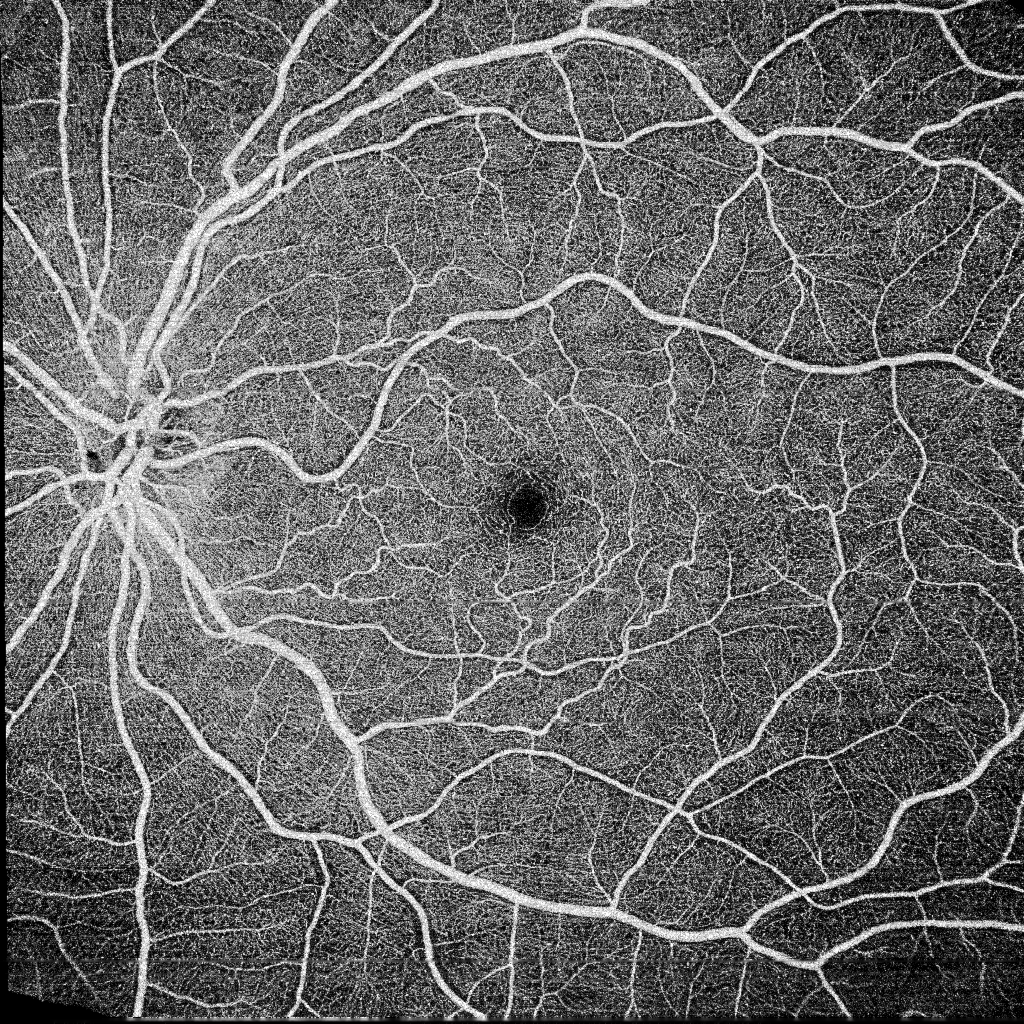
\includegraphics[width=4cm]{gambar/class0_0.png} }}%
	\subfloat[\centering Gambar \emph{heatmap} dari ResNet-18 Default Weight]{{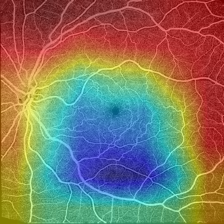
\includegraphics[width=4cm]{gambar/0_0_18def.png} }}%
	\subfloat[\centering Gambar \emph{heatmap} dari ResNet-18 Class-weighted]{{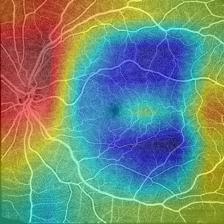
\includegraphics[width=4cm]{gambar/0_0_18class.png} }}%
	\subfloat[\centering Gambar \emph{heatmap} dari ResNet-152 Class-weighted]{{\includegraphics[width=4cm]{gambar/0_0_152.png} }}%
	\caption{Hasil \emph{heatmap} dari dataset \emph{class} 0 (Non-DR)}
	\label{fig:GRAD0}
\end{figure}

\begin{figure}[H]
	\centering
	\subfloat[\centering Gambar Asli]{{\includegraphics[width=4cm]{gambar/class1_0.png} }}%
	\subfloat[\centering Gambar \emph{heatmap} dari ResNet-18 Default Weight]{{\includegraphics[width=4cm]{gambar/1_0_18def.png} }}%
	\subfloat[\centering Gambar \emph{heatmap} dari ResNet-18 Class-weighted]{{\includegraphics[width=4cm]{gambar/1_0_18class.png} }}%
	\subfloat[\centering Gambar \emph{heatmap} dari ResNet-152 Class-weighted]{{\includegraphics[width=4cm]{gambar/1_0_152.png} }}%
	\caption{Hasil \emph{heatmap} dari dataset \emph{class} 1 (NPDR)}
	\label{fig:GRAD1}
\end{figure}

\begin{figure}[H]
	\centering
	\subfloat[\centering Gambar Asli]{{\includegraphics[width=4cm]{gambar/class2_0.png} }}%
	\subfloat[\centering Gambar \emph{heatmap} dari ResNet-18 Default Weight]{{\includegraphics[width=4cm]{gambar/2_0_18def.png} }}%
	\subfloat[\centering Gambar \emph{heatmap} dari ResNet-18 Class-weighted]{{\includegraphics[width=4cm]{gambar/2_0_18class.png} }}%
	\subfloat[\centering Gambar \emph{heatmap} dari ResNet-152 Class-weighted]{{\includegraphics[width=4cm]{gambar/2_0_152.png} }}%
	\caption{Hasil \emph{heatmap} dari dataset \emph{class} 2 (PDR)}
	\label{fig:GRAD2}
\end{figure}

Representasi fitur objek gambar lebih tersebar luas karena objek di dalam \emph{frame} adalah pembuluh darah yang memanjang dan bercabang, dibandingkan dengan entitas tunggal seperti manusia atau hewan di dalam \emph{frame} gambar.

ResNet 152 lebih mementingkan berbagai komponen gambar dibandingkan dengan ResNet 18 karena kemampuannya mempelajari representasi secara rumit. Tingkat kompleksitas yang semakin tinggi ini memungkinkan ResNet 152 mengenali fitur-fitur yang mungkin diabaikan oleh ResNet 18. Dengan mengembangkan pemahaman yang lebih luas ke analisis yang lebih mendetail, seperti dalam kasus pengenalan wajah yang mempelajari bentuk wajah hingga fitur wajah tertentu seperti alis dan kerutan, ResNet 152 menunjukkan kapasitas untuk membedakan elemen tertentu dalam sebuah gambar.
\cleardoublepage

% Bab 5 penutup
\chapter{PENUTUP}
\label{chap:penutup}

\section{Kesimpulan}
\label{sec:kesimpulan}

Berdasarkan hasil penelitian yang telah dilakukan dapat ditarik kesimpulan-kesimpulan berikut:

\begin{enumerate}[nolistsep]
	
\item Metode CNN dengan arsitektur Residual Neural Network dengan menerapkan transfer learning dapat digunakan untuk mengklasifikasikan penyakit retinopati diabetik
\item Dari masing-masing skenario, didapatkan tiga buah model yaitu best validated model dan best trained model atau model dengan validasi terbaik dan akurasi training terbaik dari 100 epoch, dan last model atau model dari epoch ke 100. Antara kedua model tersebut didapatkan bahwa best validated model menghasilkan performa lebih baik dibanding last model.
\item Tanpa menggunakan penyesuaian beban pada class, akurasi tertinggi berhasil didapatkan oleh ResNet 18 dengan akurasi 82,1%
\item Pada model dengan penggunaan penyesuaian beban \emph{class}, akurasi tertinggi berhasil didapatkan oleh ResNet 18 dengan akurasi 81,3\%
\item Pada Quadratic Weighted Kappa, best validated model memiliki nilai yang cenderung rendah disbanding dengan last model ataupun best trained model. 
\item Nilai tertinggi Quadratic weighted kappa pada model tanpa penyesuaian beban adalah resnet18 dengan nilai 0,758
\item Nilai tertinggi Quadratic weighted kappa pada model dengan penyesuaian beban adalah resnet18 dengan nilai 0,752
\item Pada best trained model, penambahan beban pada class menyebabkan perkembangan pada nilai Quadratic Weighted Kappa terkecuali pada resnet18 dan resnet 101, yang mana keduanya mengalami penurunan sebesar 0,006 dan 0,04
\item Pada best validated model, penambahan beban pada class justru menurunkan nilai Quadratic Weighted Kappa, kecuali pada resnet 50 dan resnet 101.
\item Pada model terakhir dari 100 epoch, penambahan beban pada class mengakibatkan penurunan pada nilai Quadratic Weighted Kappa kecuali pada resnet 152


\end{enumerate}

\section{Saran}
\label{chap:saran}

Berikut adalah beberapa saran yang dapat diberikan pada penelitian untuk tugas akhir ini:

\begin{enumerate}[nolistsep]
	
\item Menggunakan dataset yang lebih banyak.
\item Menggunakan fungsi tambahan untuk pemilihan pengambilan model dengan apabila terdapat lebih dari satu iterasi yang memiliki akurasi tertinggi pada suatu model.

\end{enumerate}

\cleardoublepage

\chapter*{DAFTAR PUSTAKA}
\addcontentsline{toc}{chapter}{DAFTAR PUSTAKA}
\renewcommand\refname{}
\vspace{2ex}
\renewcommand{\bibname}{}
\begingroup
\def\chapter*#1{}
\printbibliography
\endgroup
\cleardoublepage

% Biografi penulis
\begin{center}
  \Large
  \textbf{BIOGRAFI PENULIS}
\end{center}

\addcontentsline{toc}{chapter}{BIOGRAFI PENULIS}

\vspace{2ex}

\begin{wrapfigure}{L}{0.3\textwidth}
  \centering
  \vspace{-3ex}
  % Ubah file gambar berikut dengan file foto dari mahasiswa
  \includegraphics[width=0.3\textwidth]{gambar/foto diri.png}
  \vspace{-4ex}
\end{wrapfigure}

% Ubah kalimat berikut dengan biografi dari mahasiswa
\name{}, lahir di kota kecil bernama Pati pada tanggal 2 Januari 2002. Lahir sebagai anak pertama dari dua bersaudara. Setelah lulus dari SMA Negeri 1 Pati, penulis melanjutkan pendidikan ke Perguruan Tinggi Institut Teknologi Sepuluh Nopember, program studi S1 Teknik Komputer, Fakultas Teknologi Elektro \& Informatika Cerdas (FTEIC).

Selama berkuliah, penulis mengikuti kegiatan akademis yaitu Bangkit 2022 dengan \emph{path} pembelajaran komputasi awan. Penulis juga mengikuti kegiatan ekstrakurikuler yaitu staff ukm IFLS, staff UKM IAC, dan menjadi anggota dari Legislatif Mahasiswa Departemen Teknik Komputer.

Pada Penelitian tugas akhir, penulis awalnya memilih untuk mengangkat topik pembuatan gim berdasarkan sejarah. Namun dikarenakan kendala, topik tersebut tidak dapat dilanjutkan, dan penulis memilih untuk melakukan penelitian di bidan pembelajaran mesin.

%Satrio memulai pendidikannya di TK PGRI Sumbermulyo, kemudian melanjutkan pendidikan di SD Sumbermulyo 03. Pada kelas 4, SD ini memiliki murid terlalu sedikit sehingga harus diberhentikan operasionalnya. Satrio memutuskan untuk pindah ke SD Sumbermulyo 02, yang mana lebih dekat jaraknya ke rumahnya. 
%
%Setelah lulus dari SD, satrio melanjutkan pendidikannya ke SMP Negeri 1 Pati. Hal ini berbeda dengan kebanyakan teman sekelasnya yang memilih untuk melanjutkan ke SMP di daerah winong ataupun Gabus. Satrio menjadi satu-satunya murid dari desanya yang bersekolah di SMPN 1 Pati kala itu.
%
%Satrio lulus dari SMP N 1 Pati dengan Nilai UN sebesar 36,05 dan melanjutkan pendidikannya ke SMA N 1 Pati. Di sana satrio mengikuti ekstrakurikuler paskibra dan sinematografi. Sempat mengikuti OSN pada tahun 2018, namun hanya berhasil sampai ke tingkat provinsi.
\cleardoublepage

\end{document}
